\documentclass[12pt,oneside]{uhthesis}
\usepackage{subfigure}
\usepackage[ruled,lined,linesnumbered,titlenumbered,algochapter,spanish,onelanguage]{algorithm2e}
\usepackage{amsmath}
\usepackage{amssymb}
\usepackage{amsbsy}
\usepackage{caption,booktabs}
\captionsetup{ justification = centering }
%\usepackage{mathpazo}
\usepackage{float}
\setlength{\marginparwidth}{2cm}
\usepackage{todonotes}
\usepackage{listings}
\usepackage{xcolor}
\usepackage{multicol}
\usepackage{graphicx}
\floatstyle{plaintop}
\restylefloat{table}
\addbibresource{Bibliography.bib}
% \setlength{\parskip}{\baselineskip}%
\renewcommand{\tablename}{Tabla}
\renewcommand{\listalgorithmcfname}{Índice de Algoritmos}
%\dontprintsemicolon
\SetAlgoNoEnd

\definecolor{codegreen}{rgb}{0,0.6,0}
\definecolor{codegray}{rgb}{0.5,0.5,0.5}
\definecolor{codepurple}{rgb}{0.58,0,0.82}
\definecolor{backcolour}{rgb}{0.95,0.95,0.92}

\lstdefinestyle{mystyle}{
    backgroundcolor=\color{backcolour},   
    commentstyle=\color{codegreen},
    keywordstyle=\color{purple},
    numberstyle=\tiny\color{codegray},
    stringstyle=\color{codepurple},
    basicstyle=\ttfamily\footnotesize,
    breakatwhitespace=false,         
    breaklines=true,                 
    captionpos=b,                    
    keepspaces=true,                 
    numbers=left,                    
    numbersep=5pt,                  
    showspaces=false,                
    showstringspaces=false,
    showtabs=false,                  
    tabsize=4
}

\lstset{style=mystyle}

\title{Modelación de cultivos mediante el empleo de los filtros de partículas e imágenes de teledetección para la generación y selección de las mejores trayectoria de estados del cultivo.}
\author{\\\vspace{0.25cm}Eduardo Moreira González}
\advisor{\\\vspace{0.25cm}Jorge Díaz Suárez\\\vspace{0.2cm}Edel García Reyes }
\degree{Licenciado en Ciencia de la Computación}
\faculty{Facultad de Matemática y Computación}
\date{Fecha\\\vspace{0.25cm}\href{https://github.com/eduar297/thesis}{github.com/eduar297/thesis}}
\logo{Graphics/uhlogo}
\makenomenclature

\renewcommand{\vec}[1]{\boldsymbol{#1}}
\newcommand{\diff}[1]{\ensuremath{\mathrm{d}#1}}
\newcommand{\me}[1]{\mathrm{e}^{#1}}
\newcommand{\pf}{\mathfrak{p}}
\newcommand{\qf}{\mathfrak{q}}
%\newcommand{\kf}{\mathfrak{k}}
\newcommand{\kt}{\mathtt{k}}
\newcommand{\mf}{\mathfrak{m}}
\newcommand{\hf}{\mathfrak{h}}
\newcommand{\fac}{\mathrm{fac}}
\newcommand{\maxx}[1]{\max\left\{ #1 \right\} }
\newcommand{\minn}[1]{\min\left\{ #1 \right\} }
\newcommand{\lldpcf}{1.25}
\newcommand{\nnorm}[1]{\left\lvert #1 \right\rvert }
\renewcommand{\lstlistingname}{Ejemplo de código}
\renewcommand{\lstlistlistingname}{Ejemplos de código}

\begin{document}

\frontmatter
\maketitle

\begin{dedication}
    A mi familia, que tanto me ha ayudado durante toda la carrera y vida.
\end{dedication}
\include{FrontMatter/Thanks}
\include{FrontMatter/SupervisorOpinion}
\begin{resumen}
	La modelación y simulación es una herramienta que permite realizar análisis de impactos tecnológicos, económicos y ambientales, evaluar estrategias productivas y predecir con gran exactitud el rendimiento de cultivos. Al estudiar procesos de forma individual, muchas veces se pasan por alto relaciones e interacciones entre estos componentes, que gracias al uso de la simulación se pueden determinar mediante la realización de experimentos que seria muy costoso en la vida real o imposible. Esta investigación vincula la teoría con la práctica, para culminar en el desarrollo de una aplicación visual que permita, a través de la introducción de ciertos parámetros iniciales, simular el desarrollo de un cultivo y poder analizar los resultados de dicha modelación mediante el uso de gráficas y tablas.\\
	
	\textbf{Palabras clave}: simulación, modelación, cultivo, WOFOST, PCSE.
\end{resumen}

\begin{abstract}
	Modeling and simulation is a tool that allows the analysis of technological, economic and environmental impacts, the evaluation of production strategies and the accurate prediction of crop yields. When studying processes individually, relationships and interactions between these components are often overlooked, which thanks to the use of simulation can be determined by conducting experiments that would be very costly or impossible in real life. This research links theory with practice, culminating in the development of a visual application that allows, through the introduction of certain initial parameters, to simulate the development of a crop and to be able to analyze the results of such modeling through the use of graphs and tables.\\
	
	\textbf{Key words}: simulation, modeling, crop, WOFOST, PCSE.
\end{abstract}
\tableofcontents
\listoffigures
% \listoftables
% \listofalgorithms
% \lstlistoflistings

\mainmatter

\chapter*{Introducción}\label{chapter:introduction}
\addcontentsline{toc}{chapter}{Introducción}\

En Cuba uno de los sectores mas importantes es la agricultura. Su importancia radica en la necesidad de disminuir el déficit alimentario, fomentar la exportación como fuente de ingreso económica, emplear gran cantidad de trabajadores, entre otros. Sin embargo, muchas son las causas que han impedido que dicho sector alcance su máximo rendimiento; entre estas podemos citar el bloqueo económico impuesto por los Estados Unidos a nuestro país que ha imposibilitado la adquisición de maquinarias, fertilizantes, entre otras tecnologías usadas en la mayoría de los países agrícolas; la alta demanda alimenticia de la población, que a pesar de los grandes esfuerzos realizados por cumplir, en ocasiones es complicado satisfacer; las condiciones del clima que se han acuciado debido al impacto del cambio climático no solo en nuestro país, sino en el mundo.

Debido a lo expuesto anteriormente, se necesita recurrir a nuevos métodos capaces de reconocer las complejidades de naturaleza física, químicas, biológicas, así como también sociales, económicas, políticas y culturales.

El método Análisis de Sistemas o Investigación de Sistemas (\textit{System Analysis} o \textit{System Research}) garantiza una mejor comprensión de los conceptos básicos y a su vez los organiza en un marco cuantitativo y dinámico.

Gracias al gigantesco crecimiento en el campo tecnológico de la computación y la ciencia informática, contamos con herramientas dentro de la metodología antes mencionada para apoyar la integración del conocimiento adquirido en el ámbito disciplinario. Dentro de estas herramientas encontramos los modelos de simulación de cultivos, los de sistemas sociales y económicos, los de información geográfica, los de manejo de bases de datos, entre otros.

La simulación es una de las herramientas más importantes y que más disciplinas abarca, un caso particular de esta son los modelos de simulación de cultivos, los cuales tienen muchas aplicaciones de gran potencial en la actualidad en la investigación, planificación y manejo de cultivos. Estos tienen gran relevancia e importancia en la toma de decisiones en el sector agrícola dado que cuantifican, interpretan y predicen las necesidades, desarrollo y rendimiento de los cultivos.

En los últimos años estos modelos se han utilizado con grandes resultados en países de clima templado. Especialmente en países desarrollados esta herramienta cumple un papel fundamental dado su utilización en procesos como la toma de decisiones, planificación de la producción y manejo de empresas. Estas tecnologías son muy usadas también debido a que brindan una experiencia \textit{user-friendly} dado que no es necesario ser especialista para poder hacer uso de sus beneficios.


\section*{Problema}
A pesar de en los últimos años se ha implementado en nuestro país la modelación de cultivos, esta tecnología aun no es ampliamente conocida por todos. Muchos agricultores que podrían beneficiarse de esta no lo hacen por desconocimiento. Por esa razón el principal problema que se pretende resolver con este trabajo de investigación es cómo mejorar los modelos de simulación utilizados en Cuba y cómo hacer llegar esta tecnología de una forma mas fácil e intuitiva a los agricultores.

\section*{Objetivo}
Para resolver el problema planteado anteriormente, el objetivo de la tesis es la modelación de cultivos mediante el empleo de los filtros de partículas para la generación y selección de las mejores trayectoria de estados del cultivo y la implementación de una interfaz visual para el fácil manejo por los usuarios.

\section*{Preguntas científicas}
Para alcanzar este objetivo se responderán las siguientes preguntas científicas:

\begin{enumerate}
	\item ¿Cuáles son las bases teóricas necesarias para llevar a cabo el análisis?
	\item ¿Cómo se implementa un filtro de partículas?
	\item ¿Cómo se implementa la estrategia de selección de trayectorias basada en el filtro de partícula y el Índice de Área Foliar?
	\item ¿Cómo programar un modelo para la extrapolación de las trayectorias de los estados del cultivo?
	\item ¿Cómo programar un algoritmo para la estimación de rendimiento del cultivo basado en las trayectorias seleccionadas y extrapoladas?
	\item ¿Cómo implementar una aplicación web que sea intuitiva y fácil de usar por los usuarios?
\end{enumerate}

\section*{Tareas}
\begin{itemize}
	\item Investigar sobre la bibliografía necesaria para llevar a cabo la investigación.
	\item Analizar críticamente la bibliografía seleccionada.
	\item Estudio de las especificaciones y características de los modelos de simulación de cultivos.
	\item Búsqueda y selección de implementaciones computacionales de los modelos de cultivo, en especial en lenguaje Python.
	\item Estudio de los fundamentos teóricos y computacionales de los filtros de partícula.
	\item Programar un método para la codificación de trayectoria y la generación de una población de trayectorias.
	\item Programación de la estrategia de selección de trayectorias basada en el filtro de partícula y el Índice de Área Foliar.
	\item Programar un modelo para la extrapolación de las trayectorias de los estados del cultivo.
	\item Programar un algoritmo para la estimación de rendimiento del cultivo basado en las trayectorias seleccionadas y extrapoladas.
	\item Realizar experimentos de visualización de los resultados de la modelación en cultivos de campos de arroz o caña de azúcar.
	\item Desarrollo de una aplicación web para el manejo y visualización de los datos.
	\item Presentar los resultados de la investigación.
\end{itemize}

\section*{Métodos}
TODO...

\section*{Novedad e importancia práctica}
En los últimos años y gracias al desarrollo tecnológico, ha sido posible predecir las condiciones de determinado cultivo sin usar innecesariamente recursos como agua, fertilizantes o tiempo, gracias a la simulación de cultivos. Dado que esta es una tecnología muy útil, pero en cierta medida poco conocida por su novedad,  una mejora como esta podría facilitar su entendimiento y alcance, no solo por organizaciones y entidades sino también por los agricultores, que podrían beneficiarse grandemente sin tener conocimientos sobre esta. Además, este trabajo de investigación podría ser usado como referencia para futuras investigaciones en este campo.






















\chapter{Estado del Arte}\label{chapter:state-of-the-art}

\section{Sistemas, Modelos y Simulación}

Todo problema tiene un dominio en el cual se presenta y exige la construcción de un sistema, es decir, la selección y/o definición de entidades (mediante propiedades), relaciones estructurales y relaciones funcionales (entre estas entidades), las que se consideran involucradas y relevantes a la solución del problema. \parencite{temasdesimulacion} \\

Los sistemas se convierten en objeto de investigación para resolver el problema y se construyen y reconstruyen en varios niveles de abstracción según un proceso denominado modelación que suministra a diferentes niveles de abstracción representaciones estructurales y funcionales a las que se denomina modelos del sistema. El objetivo de crear modelos de un sistema tiene como fin esencialmente observar y/o modificar y/o controlar en condiciones ideales su conducta o dinámica. \parencite{temasdesimulacion} \\

La simulación es el proceso mediante el cual los procesos (dinámica) de un sistema son observados y/o modificados y controlados mediante modelos apropiados a tales fines. La dinámica de un sistema se considera simulada sólo en la medida en que esta dinámica, mediante su observación controlada, puede ser modificada con vistas a verificar principios o leyes y/o a determinar su forma más satisfactoria de realización. Siendo la computadora es el instrumento ideal para tales fines la simulación es esencialmente computacional. \parencite{temasdesimulacion} \\

De manera muy simple podemos decir que un sistema es  “[…] un conjunto de elementos relacionados entre sí y que funcionan como un todo”. \parencite{noauthor_simulacion_nodate} \\

\subsection{Sistema}

Según  \parencite{temasdesimulacion}, un sistema esta constituido por estructuras y procesos de un dominio de un problema las cuales se obtienen por abstracción a partir del dominio orientada por el problema.\\

A modo general existen varios tipos de sistemas, entre estos podemos mencionar los sistemas naturales, que están constituidos por estructuras y funciones de la realidad (átomos, partículas, sistemas biológicos); los sistemas socio-políticos, que son producto del desarrollo histórico, político y social (países, comunidades, sociedades); por último existen los denominados sistemas tecnológicos, resultado de la invención del hombre (máquinas, computadoras, sistemas eléctricos).\\

\subsubsection{Sistemas Dinámicos}

Los sistemas dinámicos son aquellos que tienen en cuenta el tiempo como dimensión fundamental y necesaria para describir su estructura, así como sus procesos. Existen dos tipos de sistemas dinámicos:
\begin{itemize}
	\item Sistema dinámico estacionario: la estructura del sistema no cambia y los procesos ocurren en el tiempo pero no se considera la dependencia del tiempo.
	\item Sistema dinámico no-e	stacionario: la estructura del sistema cambia con el tiempo y los procesos del sistema ocurren en y dependen del tiempo. \parencite{temasdesimulacion}
\end{itemize}

En esta investigación se trabajará con sistemas dinámicos a menos que el autor indique lo contrario.\\

\subsubsection{Sistema y Medio}

Un sistema existe (funciona, se desarrolla, interactúa) en un medio (ambiente). Medio es un sistema en el cual actúa, funciona, se desarrolla, con el cual interactúa en general un sistema bajo estudio. \parencite{temasdesimulacion}\\

Un sistema se considera cerrado si no se le asocia un medio, de lo contrario se le considera abierto. \parencite{temasdesimulacion}\\ Este se relaciona con su medio mediante entradas y salidas y a su vez este cambia en dependencia a su interacción con su medio.
No podemos dejar de mencionar el concepto de estado del sistema, que no es más que quien se encarga de almacenar lo mas importante de los estos cambios.
En general la acción del medio sobre un sistema (entrada) y el estado de este último son parámetros necesarios para predecir su comportamiento (estado) futuro y/o su salida o respuesta al medio. Luego, la dinámica de un sistema se describe en términos de una función de cambio de estado y una función de emisión de salida. \parencite{temasdesimulacion}\\

\subsubsection{Sistemas deterministas, no-deterministas y aleatorios}

Los sistemas se pueden distinguir en dependencia de la información que tengamos de estos, sea conocida, desconocida o parcialmente conocida (sistemas con información completa o incompleta).
Según lo anterior, un sistema se puede considerar determinista si los últimos estados de este se derivan de los anteriores o están determinados por ellos; por otra parte, se tienen los sistemas estocásticos o aleatorios en el que los estados futuros no están determinados por los anteriores.
Si un sistema es determinista, esto no implica necesariamente que los estados posteriores del sistema sean predecibles a partir del conocimiento de los anteriores. \parencite{darling_deterministic_nodate}

\subsection{Modelo}

Precisar cuáles entidades del sistema intervienen de algún modo en el problema que se desea resolver y las relaciones causales que influyen en su comportamiento y en el del sistema en su conjunto, conduce a un proceso de simplificación de la realidad, de abstracción, que se conoce como modelación.
Diferentes problemas sobre un mismo dominio da lugar a la concepción de diferentes sistemas sobre el mismo.\\

Los sistemas creados para solucionar un problema deben ser observables y/o controlables y/o modificables, o sea dado un sistema creado para resolver un problema se desea Observarlo y/o Controlarlo y/o Modificarlo. \parencite{temasdesimulacion}\\

Un modelo se utiliza para poder observar, controlar y modificar un sistema. Por lo tanto podemos definir un modelo como una descripción abstracta de un sistema que representa de forma aproximada su comportamiento.
Según \parencite{temasdesimulacion}, “Un modelo es un sistema que representa a otro sistema.”\\

Gran parte de los sistemas reales dificultan mucho que dicho modelo sea observable, controlable y modificable.\\

Podemos catalogar los modelos en dependencia de su estructura, entre estos tenemos los modelos del sistema real, a escala, analógico, matemático, computacional. En este último centraremos nuestra atención.\\

\subsubsection{Modelado Computacional}
El modelado computacional es el uso de computadoras para simular y estudiar sistemas complejos utilizando las matemáticas, la física y la informática. Un modelo computacional contiene numerosas variables que caracterizan el sistema bajo estudio. La simulación se realiza ajustando las variables, solas o combinadas, y observando los resultados. El modelado computacional permite a los científicos realizar miles de experimentos simulados por computadora. Los miles de experimentos por computadora identifican los pocos experimentos de laboratorio que tienen más probabilidades de resolver el problema bajo estudio. \parencite{noauthor_modelado_nodate}

Los modelos computacionales de hoy en día pueden estudiar sistemas muy complejos, y un caso particular de esto seria nuestro objeto de estudio, un \textbf{sistema de cultivos}, siendo este un sistema abierto, dinámico no estacionario, determinista en cierto punto con una gran porción de aleatoriedad e información la mayoría de veces incompleta. \\

\subsection{Simulación}
La simulación puede verse como la ejecución, observación y cambio de un modelo determinado.
Según la definición de Robert E. Shannon, \parencite{shannon1975simulacion} la simulación es el “[…] proceso de diseñar y desarrollar un modelo computarizado de un sistema o proceso y conducir experimentos con este modelo con el propósito de entender el comportamiento del sistema y/o evaluar varias estrategias con las cuales se puede operar el sistema”.\\

En las ciencias, la simulación es el artificio contextual que referencia la investigación de una hipótesis o un conjunto de hipótesis de trabajo utilizando modelos.
Simulación es una técnica numérica para conducir experimentos en una computadora digital. Estos experimentos comprenden ciertos tipos de relaciones matemáticas y lógicas, las cuales son necesarias para describir el comportamiento y la estructura de sistemas complejos del mundo real a través de largos periodos de tiempo. \parencite{noauthor_simulacion_nodate}\\

La simulación computacional es la basada en modelos computacionales.

Los recientes avances en las metodologías de simulación y la gran disponibilidad de diversos tipos de software existentes en el mercado han hecho que la técnica de simulación sea una de las herramientas más ampliamente usadas en el \textbf{análisis de sistemas}.

Gracias a los avances tecnológicos una computadora puede tomar el papel de cualquier máquina o sistema existente. A medida que aumenta la complejidad del sistema mas se dificulta para la computadora replicar dicho comportamiento, por lo tanto es necesario emplear modelos del sistema simplificado, tomando solo de este lo que sea relevante para el análisis.

\subsubsection{Modelado de sistemas complejos}

En la actualidad, debido a los avances tecnológicos del microprocesador, han nacido nuevas técnicas de modelado de sistemas complejos, entre estas podemos mencionar dos grandes exponentes que son la simulación basada en agentes y la dinámica de sistemas. Ambas complementan modelos no formales de sistemas complejos y modelos matemáticos con un mayor nivel de abstracción.\\

Varios filósofos como Hesse \parencite{echenique1970models} y Hughes \parencite{hughes1997models} proponen un esquema general del proceso científico. Estos modelos se construyen para desarrollar procesos de inferencia sobres algunos aspectos de sistemas reales observados con anterioridad. Tomando como base estos procesos de inferencia se mejora la forma de entender los sistemas reales observados. \parencite{izquierdo2008modelado}

En la figura (\ref{fig:img_1}) se muestra el proceso de creación y uso de un modelo.

\begin{figure}[!h]
	\centering
	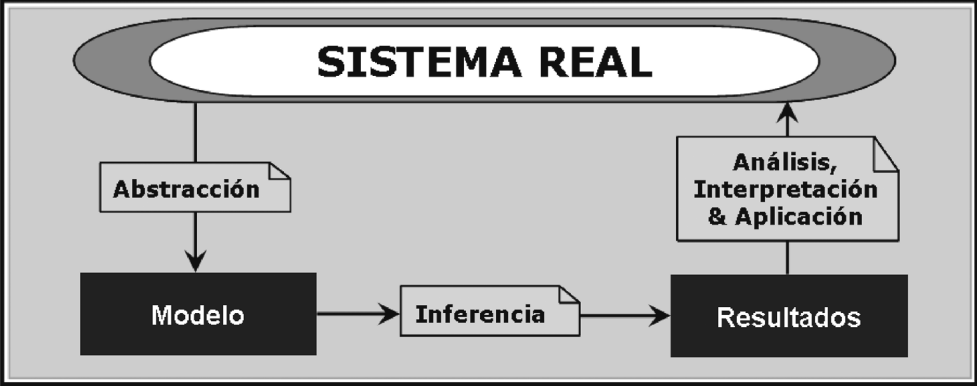
\includegraphics[scale=0.5]{Images/esquema_modelado_cientifico.png}
	\caption{Esquema general del proceso de modelado científico. \parencite{izquierdo2008modelado}}
	\label{fig:img_1}
\end{figure}

Se puede concluir que luego de analizar un modelo, se llegaran a conclusiones que no serán estrictamente rigurosas respecto a lo que sucede en el sistema real. Sin embargo, con la aplicación del modelo se obtendrán conocimientos que sin esta no hubiese sido posible adquirir.\\

Como se observa en la figura (\ref{fig:img_1}), el proceso de modelado no es unidireccional ya que generalmente se suele diseñar un modelo, del cual se obtienen resultados, teniendo en cuenta estos se perfecciona el modelo mediante ciertos cambios lógicos en sus valores iniciales o intermedios. El modelo inicial puede haber fallado por dos motivos fundamentales:
\begin{itemize}
	\item porque no parecieran derivarse lógicamente de las premisas del modelo (proceso de verificación).
	\item porque, aún siendo lógicamente correctos, difirieran excesivamente de los resultados observados en el sistema real que se está modelando (proceso de validación). \parencite{izquierdo2008modelado}
\end{itemize}

De una manera un tanto informal, podríamos decir que verificar consiste en valorar si el modelo que tenemos es correcto, mientras que validar consiste en estudiar si tenemos el modelo correcto.\\


Los sistemas complejos (p. ej. organismos pluricelulares, colonias de hormigas, ecosistemas, economías, sociedades…) están caracterizados por tener una estructura compuesta por varios niveles. En estos sistemas complejos \parencite{vicsek2002complexity, gilbert2004agent}:

\begin{itemize}
	\item Los componentes de niveles jerárquicos inferiores suelen mostrar un grado de autonomía significativo.
	\item El comportamiento del sistema surge a partir de la auto-organización de sus componentes, sin que esta organización esté controlada ni dirigida por ningún ente exterior al sistema.
	\item Los componentes básicos de estos sistemas complejos (células, hormigas, individuos, poblaciones, empresas…) perciben su entorno y responden a cambios en él de forma potencialmente diferente.
\end{itemize}

Todas estas características hacen que el proceso de modelado formal de sistemas complejos difiera sustancialmente del de otros sistemas más simples. En particular, su naturaleza descentralizada, la presencia de bucles de causalidad y retroalimentación no lineales, y el hecho de contener varias unidades más o menos autónomas, que pueden interaccionar, evolucionar, y adaptar su comportamiento a cambios en el entorno, implica que en la mayoría de los casos es muy difícil, si no imposible, conseguir un modelo que pueda describir el sistema complejo adecuadamente y que además sea resoluble matemáticamente. \parencite{izquierdo2008modelado}\\

Un modelo computacional es un modelo formal (que por lo tanto puede expresarse en lenguaje matemático como un conjunto de ecuaciones), y la simulación computacional es una herramienta que nos permite estudiarlo más allá de los límites actuales de las matemáticas. De este modo, el resultado final es un modelo potencialmente más realista, y que todavía conserva el rigor formal de los modelos matemáticos más tradicionales. \parencite{izquierdo2008modelado}\\

Luego de analizada la posibilidad de trabajar con modelos formales de mayor complejidad, se hace necesario ampliar el esquema visto en la figura (\ref{fig:img_1}) a la siguiente (\ref{fig:img_2}):

\begin{figure}[!h]
	\centering
	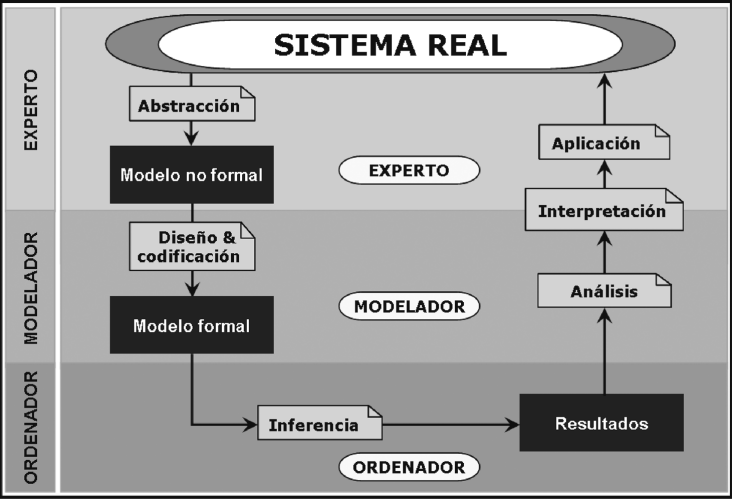
\includegraphics[scale=0.5]{Images/esquema_modelado_cientifico_con_abstraccion.png}
	\caption{Proceso de modelado con abstracción intermedia. \parencite{izquierdo2008modelado}}
	\label{fig:img_2}
\end{figure}

\subsubsection{Simulación basada en agentes}

La simulación basada en agentes (agent-based modelling) es un novedoso método de investigación para las ciencias sociales. Dicho método fue inicialmente desarrollado en el campo de la IA (Inteligencia Artificial) a lo largo de la década de los 50 del pasado siglo y ha sido empleado desde entonces para resolver algunos de los problemas propios de las ciencias físicas y naturales. Sin embargo, ha empezado a utilizarse recientemente en las ciencias sociales, aunque su objeto de estudio difiera de los de las ciencias físicas y naturales. \parencite{garcia2016simulacion}\\

Mediante la simulación basada en agentes, el modelador reconoce
explícitamente que los sistemas complejos, y en particular los sociales, son
producto de comportamientos individuales y de sus interacciones. \parencite{izquierdo2008modelado}
Este tipo de simulación se distingue de de otras por la forma en que se construye la primera abstracción del sistema real y por tanto del modelo formal.\\

Se caracterizan por comprender varios agentes que son, en mayor o menor grado, autónomos, heterogéneos e independientes, que muestran cada uno sus propias metas y objetivos, y que generalmente son capaces de interaccionar entre sí y con su entorno \parencite{torsun1995foundations}. En muchas ocasiones, pero no siempre, son sistemas caracterizados por la existencia de un número grande de agentes relativamente simples, que pueden evolucionar a lo largo del tiempo para adaptarse a nuevas condiciones del entorno o a nuevos objetivos. \parencite{izquierdo2008modelado}

A continuación se pueden ver los cuatro tipos básicos de agentes encontrados en casi todos los sistemas inteligentes:
\begin{itemize}
	\item Agentes reactivos simples: son el tipo de agente más sencillo. Estos agentes seleccionan las acciones sobre la base de las percepciones actuales, ignorando el resto de las percepciones históricas.
	\item Agentes reactivos basados en modelos: La forma más efectiva que tienen los agentes de manejar la visibilidad parcial es almacenar información de las partes del mundo que no pueden ver. O lo que es lo mismo, el agente debe mantener algún tipo de estado interno que dependa de la historia percibida y que de ese modo refleje por lo menos alguno de los aspectos no observables del estado actual.
	\item Agentes basados en objetivos: El conocimiento sobre el estado actual del mundo no es siempre suficiente para decidir qué hacer. En otras palabras, además de la descripción del estado actual, el agente necesita algún tipo de información sobre su meta que describa las situaciones que son deseables.
	\item Agentes basados en utilidad: Las metas por sí solas no son realmente suficientes para generar comportamiento de gran calidad en la mayoría de los entornos. Las metas sólo proporcionan una cruda distinción binaria entre los estados de «felicidad» y «tristeza», mientras que una medida de eficiencia más general debería permitir una comparación entre estados del mundo diferentes de acuerdo al nivel exacto de felicidad que el agente alcance cuando se llegue a un estado u otro. Como el término «felicidad» no suena muy científico, la terminología tradicional utilizada en estos casos para indicar que se prefiere un estado del mundo a otro es que un estado tiene más utilidad que otro para el agente. \parencite{russell2004inteligencia}
\end{itemize}
Puesto que el énfasis en la simulación basada en agentes está en encontrar abstracciones apropiadas que describan los componentes básicos del sistema y sus interacciones (en vez de buscar abstracciones que versen directamente sobre la dinámica global del sistema), esta técnica de modelado es particularmente útil para modelar procesos emergentes de forma natural.\parencite{izquierdo2008modelado}

\subsubsection{Simulación basada en dinámica de sistemas}

La dinámica de sistemas, situada en la misma área de conocimiento que la teoría general de sistemas, la automática y la cibernética, nació de la aplicación —realizada en la década de los 50 por Jay W. Forrester, de la teoría de los bucles de realimentación a un caso concreto de gestión industrial. Aplicada en 1970 al estudio del mundo como sistema dinámico,  esta metodología, cuyo objetivo es construir modelos dinámicos de sistemas sociales basándose en la opinión de expertos y el uso de la simulación con computadores, es actualmente una  herramienta que cubre un amplio campo de aplicaciones, desde la  gestión de empresas hasta la construcción de modelos urbanos, regionales, sociológicos y ecológicos. \parencite{aracil1997dinamica} \\

La dinámica de sistemas es otra técnica de modelado de sistemas complejos. También se utiliza para modelar sistemas en ingeniería \parencite{ford1997system, ford1998dynamic}, economía y negocios \parencite{bayer2004sterman, ellis2007impacto}, entre otros. \parencite{izquierdo2008modelado}.

Esta tiene como base el concepto de retroalimentación, o causalidad circular entre variables observables.
A diferencia de la simulación basada en agentes, el centro de la dinámica de sistemas está en la relación que existe entre las variables observables.
Por tanto la idea central de este modelo de simulación está en encontrar las variables críticas del sistema complejo e identificar los vínculos causales existentes entre ellas.

\section{Modelos de Simulación de Cultivos}

Los modelos de simulación son una herramienta fundamental para entender la complejidad de los sistemas ecológicos y ambientales como bien se plasmó anteriormente.
Un buen modelo es capaz de revelar interacciones entre los diferentes componentes que no eran evidentes al estudiar cada uno de los procesos separadamente y permitirá llevar a cabo experimentos, que no se podrían realizar en el sistema real dado que pueden ser muy costosos en términos de trabajo, recursos o tiempo.
Sin perder generalidad, una de las funciones que estos permiten, es la de analizar, pronosticar e incluso mejorar el rendimiento de los cultivos.
Dichos modelos tienen varias aplicaciones potenciales en la actualidad en respuesta a temas que guardan relación con la investigación, manejo y planificación de cultivos. Estos juegan un papel importante en la toma de decisiones en la agricultura al cuantificar, interpretar y predecir las necesidades hídricas de los cultivos, su desarrollo y rendimiento. \parencite{granmaEMFord}
Durante las últimas décadas se han aplicado estos modelos en países de clima templado debido a los grandes beneficios que aportan.\\

Como un modelo no es más que una representación simplificada de un sistema, y un sistema es una parte bien delimitada de la realidad, se puede ver un sistema de cultivo como el cultivo en sí con todos sus órganos, o sea, raíz, tallo y hojas, sus procesos y mecanismos como el crecimiento, desarrollo, fotosíntesis, transpiración, entre otros. \parencite{hernandez2009modelos}

La modelación empezó a aumentar su importancia en el sector de la agronomía dada su capacidad de brindar información de manera periódica de todo el sistema biológico o una parte, como es el sistema de producción agrícola. \parencite{guevara2007simulacion}

Una sabia utilización de los recursos en la actualidad implica una mayor probabilidad de aumento de la producción alimenticia. Además, el cambio climático, la variabilidad del clima, suelo, el secuestro de carbono a largo plazo, efectos en la seguridad alimentaria y la sostenibilidad del medio ambiente se han convertido en aspectos importantes a tener en cuenta. Por otra parte, la agricultura de los países tropicales enfrenta cada vez más nuevos retos, debido a cambios en las políticas macroeconómicas, al crecimiento de la población, el bajo rendimiento y a los límites de sostenibilidad de los recursos naturales utilizados en la producción. Conocer adecuadamente la dinámica y los efectos de los principales factores involucrados en el desarrollo agrícola, para poder elaborar alternativas viables de progreso en nuestros trópicos americanos, conservando los recursos naturales mediante su utilización racional, son aspectos de especial importancia y deben ser objeto prioritario de actualización profesional. Cada día resulta más crucial la necesidad de la información en la toma de decisiones y existe un vacío importante entre la información que se necesita y la que se genera tradicionalmente mediante la investigación disciplinaria. Para este propósito una herramienta como los \textbf{modelos de simulación de los cultivos} es de gran utilidad.  \parencite{hernandez2009modelos}

Los modelos de simulación son una herramienta que facilitan la toma de decisiones, para seleccionar la mejor alternativa que se puede lograr con una combinación de recursos y precios, y muestra cuánto se podría pagar por una unidad más de cada recurso que se agota. \parencite{holmann2002uso}\\

En la década del 50 aparecen los modelos de simulación, luego a mediados de los 60 aparece el concepto de sistemas dinámicos, que como se vio en anteriores secciones, incluyen la variable tiempo y representan el flujo de esos procesos y sus interacciones. En esta última etapa, destacan dos importantes pioneros, W. G. Duncan en la University of Kentucky y C. T. de Wit en la Agricultural University de Wageningen, que desarrollaron modelos como herramienta para explicaciones científicas, como por ejemplo, sintetizar y mejorar la comprensión de procesos tales como la intercepción de radiación y fotosíntesis, desarrollando modelos simples que consideraban únicamente la producción potencial relacionada con la radiación y la temperatura. En la década del 70 se formaliza aquel concepto de dinámica de sistemas y en los 80 se refina mediante técnicas de computación la verificación, validación y evaluación de esos modelos. 
En esta última década aparecen los primeros modelos de simulación para los cultivos de maíz, soja, trigo y arroz, incluidos en el paquete DSSAT (Decision Support System for Agrotechnology Transfer) “Sistema de apoyo para las decisiones de transferencia agrotecnológica”.
La simulación de sistemas agrícolas comenzó a ser una herramienta fundamental para la integración de los diferentes componentes productivos dentro de los sistemas agrícolas. \parencite{hernandez2009modelos}

Los avances en el conocimiento de las interacciones dentro del ecosistema, influenciado por el ambiente y por las prácticas de manejo, expandió la potencialidad de uso de esta herramienta como ayuda para la toma de decisiones. \parencite{barrett2018humanization}

A mediados de los 90 gana auge la tecnología informática permitiendo una mayor utilización de estos modelos para el estudio y resolución de problemas específicos como el desarrollo y crecimiento de los cultivos, evaluación de respuesta a la fertilización, estrategias de riego, situaciones de estrés, predicción de pérdidas por erosión, lixiviación de pesticidas, contaminación del ambiente, calentamiento global de la atmósfera, entre otros. \parencite{guevara2007simulacion}

En general, son aceptables los puntos de vista de los que aseveran que la implementación de los modelos de simulación para las ciencias agrícolas y biológicas y sus usos prácticos está en un momento de gran importancia. \parencite{galvez2008modelacion}

\subsection{Modelos, Características y su Utilización}

En la actualidad se cuenta con una rica fuente de datos y conocimiento dentro de cada campo en particular, debido a esto se desarrollan modelos con distintos niveles de complejidad. La clasificación de los modelos ha sido intentada anteriormente, pero no se pueden hacer delimitaciones definidas, ya que los modelos generalmente poseen características de más de un grupo. \parencite{galvez2008modelacion, hernandez2009modelos}\\

Se pueden clasificar estos modelos de simulación en dos grupos:
\begin{enumerate}
	\item Empíricos: son descriptivos, se derivan de datos observados sin involucrar procesos fisiológicos y tienen escasa capacidad explicativa.
	\item Mecanicistas: poseen capacidad explicativa de la fisiología del cultivo, porque consideran aspectos como la temperatura, la radiación fotosintéticamente activa, el índice de área foliar, la fotosíntesis, la respiración y la eficiencia en el uso de la radiación. \parencite{refugio2004modelos}
\end{enumerate}

Dentro de estas clasificaciones existen otras categorías, que de acuerdo a sus características han sido nombradas de diferente forma.
Los modelos que estudian las relaciones biológicas para describir el comportamiento de un sistema son denominados modelos mecanísticos, a diferencia de los modelos empíricos que describen las relaciones matemáticas entre los datos. \parencite{vargas2004modelo}.

\textbf{Modelos empíricos o descriptivos}: Estos modelos describen, de un modo simplificado, el comportamiento de un cultivo.
El desarrollo de un modelo empírico se basa en la individualización, a partir de datos experimentales, de una o más ecuaciones matemáticas, para la representación del proceso examinado. Las principales carencias de este tipo de aproximación son las de investigar en la limitada validez en ambientes diversos a los originales y en el empleo de las ecuaciones que a menudo no tienen un significado biológico \parencite{bandi2003instrumentos}

Los modelos empíricos son descripciones directas de los datos observados y se expresan generalmente como ecuaciones de regresión (con uno o varios factores) y se utilizan para estimar la producción final. Ejemplos de tales modelos incluyen la respuesta de la producción a la aplicación de fertilizantes, la relación entre el área de la hoja y la cantidad de hojas de una planta dada, la relación entre la altura del tallo y el número de tallos, su diámetro y la producción final de caña de azúcar. \parencite{galvez2008modelacion}

\textbf{Modelos mecanísticos}: Estos modelos son aquellos que describen el comportamiento del sistema en términos de propiedades de bajo nivel. Por tanto, existe comprensión o explicación en los niveles inferiores. Estos modelos tienen la habilidad de imitar importantes procesos físicos, químicos o biológicos, y describir cómo y por qué resulta una respuesta particular. El analista comienza usualmente con algún empirismo y en la medida que se gana en conocimiento se introducen variables y parámetros adicionales para explicar la producción de la cosecha. Así, el analista adopta un enfoque reduccionista. La mayoría de los modelos de crecimiento de cultivos caen dentro de esta categoría. \parencite{galvez2008modelacion}

\textbf{Modelos estáticos y dinámicos}: Los modelos estáticos representan relaciones entre las variables que no se modifican en el tiempo y, por tanto, se conoce su valor final y no su evolución en el tiempo (por ejemplo la simulación de la intercepción solar, fotosíntesis). \parencite{bandi2003instrumentos}

Los modelos dinámicos describen el modo en el cual el sistema cambia en el tiempo y, por lo tanto, es posible seguir la evolución temporal de cada una de las variables del sistema (por ejemplo el balance de nitrógeno y agua en el suelo). \parencite{bandi2003instrumentos}

\textbf{Modelos determinísticos y estocásticos}: Los modelos determinísticos atribuyen un solo valor a cada variable del sistema. \parencite{bandi2003instrumentos} Hacen predicciones para cantidades (por ejemplo, producción de la cosecha) sin ninguna distribución probabilística asociada, varianza o elemento aleatorio. En los sistemas biológicos y agrícolas son normales las variaciones, debido a imprecisiones en los datos recogidos y a heterogeneidad del material con que se ha trabajado. En algunos casos, los modelos determinísticos pueden ser adecuados a pesar de estas variaciones inherentes, pero en otros pueden resultar insatisfactorios, por ejemplo, en la predicción de lluvia. Cuanto mayor sea la incertidumbre del sistema, más inadecuados se vuelven los modelos determinísticos. \parencite{galvez2008modelacion} Los modelos estocásticos señalan, en cambio, para una variable una distribución de valores. \parencite{bandi2003instrumentos}

Cuando la variación y la incertidumbre alcanzan un nivel alto, se hace recomendable desarrollar un modelo estocástico que dé un valor medio esperado con una varianza asociada. Sin embargo, los modelos estocásticos tienden a ser difíciles de manipular y rápidamente se vuelven muy complejos. Por consiguiente, es recomendable intentar resolver el problema inicialmente con un enfoque determinístico y utilizar el enfoque estocástico sólo si los resultados no son adecuados o satisfactorios. \parencite{galvez2008modelacion, hernandez2009modelos}

Para el procesamiento y análisis de la problemática, utilizando análisis de regresión, es necesario considerar \parencite{fernandez2003biomodelos, rodriguez2018aplicaciones}:
\begin{itemize}
	\item Ploteo de puntos para analizar tendencia de datos.
	\item Selección del tipo de modelo a ajustar.
	\item Ajuste del modelo, con el apoyo de un software apropiado.
	\item Descripción del proceso a partir del modelo obtenido.
\end{itemize}

En estos estudios se requiere de una labor eficiente en la organización y desarrollo de la investigación científica y el conocimiento que esta genera, a lo que puede contribuir en gran medida la aplicación consecuente de estos modelos, con el apoyo de las nuevas tecnologías de la información y la comunicación. Igualmente, con mucha frecuencia, no se valoran los supuestos teóricos de los modelos estadísticos y no se establecen conclusiones válidas a partir de la información analizada. \parencite{guerra2003criterios}:
\begin{itemize}
	\item Métodos de ajuste de los modelos.
	\item Error estándar de los estimadores de los parámetros (Test t de Student).
	\item Coeficiente de variación de los estimadores.
	\item Límites de confianza de los parámetros.
	\item Test de redundancia de los parámetros.
	\item Análisis de varianza relacionado con el modelo en cuestión.
	\item Coeficiente de determinación $R^2$ y $R^2$ ajustado por los grados de libertad, para modelos con diferentes números de parámetros.
	\item Suma de cuadrados o Cuadrado Medio Residual.
	\item Error estándar de estimación.
	\item Test de falta de ajuste del modelo.
	\item Análisis del efecto del uso de transformaciones en el modelo.
	\item Diagnóstico y tratamiento de la multicolinealidad, en modelos de regresión lineal múltiple.
	\item Validación de las predicciones del modelo.
	\item Estadístico PRESS (Suma de Cuadrados del Error de Predicción).
	\item Estadístico CMEP (Cuadrado Medio del Error de Predicción).
	\item Estadístico Cp de Mallows.
	\item Coeficientes de correlación entre los resultados predichos y los reales.
	\item Análisis de la precisión de las estimaciones.
	\item Análisis de los residuos.
	\item Normalidad (Test de ShapiroWilks, Kolmogorov-Smirnov).
	\item Autocorrelación (Test de Rachas, Signos, DurbinWatson, $X^2$ de independencia, Ljung y Box).
	\item Homocedasticidad (Gráficos de los residuos, Test de Cochran, Bartlett y Hartley).
\end{itemize}

\subsection{Aplicaciones de Modelos y Simulación de cultivos agrícolas en Cuba}

Desde la década de los 80 se ha venido utilizando la modelación por algunos investigadores cubanos con el objetivo de describir el crecimiento de cultivares. En el Instituto Nacional de Ciencias Agrícolas (INCA) se realizaron comparaciones entre varias funciones matemáticas para describir el crecimiento de algunos órganos en posturas de café crecidas en vivero \parencite{soto1986crecimiento}. Se determinó, además, la influencia del uso o no de la sombra durante el período de aviveramiento, la altura sobre el nivel del mar y dos fechas de siembra, en la dinámica de crecimiento de plántulas de cafeto \parencite{soto1991dlnamlca, hernandez2009modelos, rodriguez2018aplicaciones}.

También se han comparado modelos para medir la respuesta a dosis de nitrógeno en maíz y cafeto. Lo cual demostró que un modelo discontinuo rectilíneo resulta más adecuado en el sistema de recomendación de dosis óptimas de fertilizantes nitrogenados para estos cultivos, en comparación al modelo curvilíneo, que brinda dosis óptimas superiores, que implican un menor factor parcial de productividad de la dosis recomendada \parencite{martin2016comparacion, rodriguez2018aplicaciones}.

Otros trabajos aplicaron herramientas de modelación para el análisis de las respuestas de las interacciones planta-ambientemanejo en distintos escenarios de la producción de arroz, maíz, sorgo y trigo en Cuba \parencite{hernandez2016utilizacion}; demostrando que estas permiten establecer estrategias para el desarrollo de los cultivos estudiados en escenarios futuros y en otras condiciones de cultivo. Por primera vez en el país, se cuenta con información para poder predecir el comportamiento y rendimiento de estos cereales. Demuestran además que el modelo DSSAT puede ser utilizado para las condiciones de Cuba en los indicadores de rendimiento y sus componentes. \parencite{rodriguez2018aplicaciones}.

Por los beneficios que aportan los modelos determinísticos, especialistas de la Universidad Agraria de La Habana y del Instituto Nacional de Riego y Drenaje, elaboran los primeros trabajos para utilizar, en las condiciones geográficas de Cuba, cinco de los modelos agrohidrológicos de alcance internacional. Por primera vez en Cuba se brindan los parámetros que describen las propiedades hidráulicas para los principales grupos de suelos cubanos. Esta investigación le confiere validez al modelo SWACROP para ser utilizado en el cultivo de la papa en condiciones tropicales \parencite{ruiz1997utilizacion, rodriguez2018aplicaciones}.

Algunos trabajos se han realizado, durante varios años, en la evaluación y validación de diferentes modelos de simulación de transferencias hídricas para las condiciones edafoclimáticas de la región sur de La Habana (actualmente Mayabeque y Artemisa). Estas investigaciones pretenden resumir y discutir las principales características de los modelos de simulación STIC y MACRO y sus posibilidades para la predicción del comportamiento de los cultivos agrícolas ante diferentes manejos de agua, fertilización y ambientes climáticos. \parencite{lopez20143, robaina2013crop, rodriguez2018aplicaciones}

También se ha utilizado la modelación matemática con el fin de estudiar el crecimiento del diámetro medio, la altura media y el volumen por hectárea de \textit{Pinus caribaea morelet var.}
\textit{Caribaea barret} y \textit{golfari }en la Unidad Silvícola “Los Jazmines” de Viñales y en la Empresa Forestal Integral “La Palma” \parencite{suarez2011modelacion, sarria2013modelacion}. Donde se determinaron los modelos que mejor describen el comportamiento de las variables estudiadas en cada uno de los escenarios. \parencite{rodriguez2018aplicaciones}

La aplicación a la producción de pastos y forrajes, tuvo sus inicios en pasto estrella (C. nlemfuensis) \parencite{del1998analisis, torres1999empleo}, donde se encontraron relaciones polinómicas entre las variables; pero en estos modelos los parámetros no tienen interpretación biológica. Posteriormente se modeló y simuló el comportamiento productivo del pasto estrella (C. nlemfuensis) bajo diferentes frecuencias de corte, niveles de fertilización y condiciones climatológicas adversas para el desarrollo de este cultivo \parencite{rodriguez2020modelacion}. El modelo Gompertz utilizado ajustó los datos con coeficientes de determinación que estuvieron alrededor del $99 \% $ para los períodos lluvioso y poco lluvioso. Además pronostica que un incremento de la temperatura media del planeta en 2 y 4 ºC afectará el rendimiento de materia seca acumulada de este cultivo principalmente en el período poco lluvioso. \parencite{rodriguez2018aplicaciones}

Otros autores estudiaron la dinámica de acumulación de biomasa del king grass (P. purpureum) o de algunos de sus clones con el empleo de modelos no lineales \parencite{diaz2007evaluacion, noda2013modelacion}. Además, en cultivares de Brachiaria, Panicum y Pennisetum y en variedades de Tithonia diversifolia, se evaluaron diferentes modelos y encontraron ajustes lineales para las variables en estudio \parencite{ramirez2012rendimiento, torres2012utilizacion, rodriguez2018aplicaciones}.

\subsection{Modelos de Cultivo más Conocidos}

Los modelos de simulación agronómica son herramientas que integran información, y permiten analizar y cuantificar las relaciones existentes entre los factores mencionados y sus efectos como componentes del sistema, para evaluar diferentes planteos productivos o analizar un factor manteniendo los otros constantes; por ejemplo, la variación del rendimiento por efecto del clima sin modificar el manejo, el genotipo y el suelo. Numerosos modelos han sido desarrollados por diferentes grupos de trabajo y cada uno de ellos tiene fortalezas y debilidades para predecir las variables de respuesta. Es por ello necesario validar los modelos en los ambientes en donde se utilizarán \parencite{salvagiotti2003analisis}.

No obstante la capacidad relativa de los modelos existentes y la credibilidad de sus resultados es todavía un aspecto importante a valorar. Esto está asociado primeramente a la no disponibilidad de datos apropiados para la validación del modelo y, por otra, a la inadecuación en las representaciones de los procesos e interacciones del sistema agua-suelo-planta-atmósfera. Es por tanto muy importante antes de adoptar uno u otro modelo para aplicaciones agrícolas y medioambientales que se realice un trabajo de evaluación y validación exhaustivo de estos \parencite{lopez20143}.\\

\textbf{DSSAT}: (Sistema de Apoyo de Decisiones para la Transferencia de la Agrotecnología). Desde 1983, un grupo internacional de científicos cooperantes han desarrollado modelos de simulación de cultivos, enfocados a proporcionar estimaciones realistas del comportamiento de los cultivos bajo diferentes estrategias de manejo y condiciones ambientales. Estos modelos se han combinado en un paquete, como parte de un programa de enlaces (software shell) conocido como Sistema de Apoyo para Decisiones de Transferencia de Agrotecnología (DSSAT, por sus siglas en inglés) \parencite{jones1998decision}.
Los modelos de simulación de cultivos del DSSAT utilizan archivos de datos para clima, suelo y manejo del cultivo. Estos archivos se utilizan para proveer en la simulación un ambiente parecido a donde crece el cultivo. El DSSAT, además, incluye varios programas de aplicación para análisis estacionales \parencite{thornton1994computer}, rotación de cultivo y análisis secuencial \parencite{thornton1995computer}, y análisis espacial a escala de campo o regional \parencite{engel1997aegis, thornton1997computer}. Los modelos proveen una de las mejores aproximaciones del comportamiento de los cultivos, integrando nuestro entendimiento de los procesos complejos de las plantas influenciados por el clima, el suelo y las condiciones de manejo \parencite{white2003gene}.
El modelo DSSAT ha sido usado por investigadores de todo el mundo en los últimos 15 años; este paquete tiene incorporado 16 modelos de cultivos diferentes, con un software que facilita la evaluación y aplicación de estos modelos de cultivos para diferentes propósitos \parencite{jones2003dssat}. Estos permiten simular el crecimiento de cultivos de importancia económica y han demostrado alta confiabilidad en distintas condiciones de clima, suelo y manejo \parencite{jones1993decision}. Con este modelo es posible organizar y archivar bases de datos sobre clima, suelos, cultivos, experimentos y precios; simular producciones de cultivo en una o varias épocas y en secuencias; analizar resultados y representar gráficamente simulaciones; analizar variabilidad espacial y evaluar diferentes prácticas de manejo específicas a una explotación o parte de ella \parencite{giraldo2007adaptacion}.\\

\textbf{UNSAT}: El software UnSat Suite Plus combina los modelos HELP, PESTAN, SESOIL, VLEACH y VS2DT en un nuevo ambiente gráfico de gran alcance, diseñado específicamente para simular el flujo del agua subterránea y el transporte unidimensional del contaminante con la zona no saturada. Este modelo unidimensional simula el flujo vertical descendente de aguas subterráneas, así como la migración de contaminantes disueltos en aguas subterráneas, a través de una fina columna de suelo.

El paquete de software UnSat Suite Plus incluye numerosas herramientas y elementos de diseño que le permitirán producir simulaciones de flujo profesionales. Las funciones de este producto incluyen:

\begin{itemize}
	\item Entorno de modelado unificado.
	\item Nuevo asistente de proyectos.
	\item Gestión de proyectos.
	\item Datos de entrada.
	\item Visualización gráfica.
	\item Enlaces de la base de datos.
	\item SWS Weather Generator.
	\item Integración perfecta.
	\item Presentación de resultados.
	\item Generador de informes automático.
\end{itemize}

Las funciones de simulación se posibilitan gracias a la integración de 5 modelos diferentes dentro del software de UnSat Suite plus. Estos modelos que se integran son:
\begin{itemize}
	\item HELP, es un modelo aplicable a los procesos hidrológicos de taludes, terraplenes, desmontes, laderas modificadas, etc., permitiendo comprobar la estabilidad, viabilidad y correcto diseño del mismo. También es eficaz en el cálculo del valor de la recarga del agua subterránea.
	\item PESTAN (PESTticide ANalítico), es un modelo analítico de pesticidas, que utiliza una solución analítica para predecir el transporte de solutos orgánicos con la zona no saturada a la tabla del agua subterránea. Resulta útil para evaluar el potencial para la contaminación del agua subterránea por los pesticidas usados en usos agrícolas, así como impactos potenciales del agua subterránea de cualquier soluto orgánico que emigra con la zona no saturada.
	\item SESOIL (Flujo estacional y modelo de transporte para la zona de SUELO insaturada), es un modelo capaz de simular, simultáneamente, el movimiento del agua, transporte de sedimento y el agente contaminante en el terreno. Se utiliza para la investigación en el transporte del contaminante, el lavado del mismo, volatilización y difusión en el aire de la parte volátil, así como los fenómenos de absorción, volatilización, degradación, intercambio catiónico, hidrólisis y complejación del metal.
	\item VLEACH (Modelo de lixiviación de zonas no saturadas), es un modelo de la lixiviación unidimensional de la zona no saturada, mediante un modelo de diferencias finitas, el cual predice el movimiento y migración vertical de contaminantes orgánicos en la zona no saturada. Esto permite evaluar los daños en el agua subterránea debido a la migración vertical del contaminante por la zona no saturada y predecir la volatilización en la subsuperficie de los posibles volátiles.
	\item VS2DT (Modelo de transporte y flujo en 2D variablemente saturado), es un modelo numérico de diferencias finitas para flujo de estado estacionario o transitorio. Los usos típicos del modelo de VS2DT incluyen la determinación el sino de productos químicos agrícolas, lavado del terraplén, fugas y vertidos accidentales de productos químicos, mientras que emigran con la zona no saturada hacia la zona saturada del acuífero.
\end{itemize}

Cuenta con las siguientes aplicaciones: simular el transporte y el destino a largo plazo de contaminantes (COV, HAP, pesticidas y metales pesados) en la zona insaturada con condiciones variables en función de la estación utilizando SESOIL; predecir la migración vertical de los hidrocarburos volátiles a través de la zona vadosa con condiciones de flujo de estado permanente utilizando VLEACH; calcular la migración de pesticidas agrícolas a través de zonas insaturadas con condiciones de flujo de estado permanente utilizando PESTAN; simular el flujo de aguas subterráneas y los procesos de transporte de contaminantes a través de suelos insaturados heterogéneos con condiciones de flujo variable utilizando VS2DT; generar hasta 100 años de datos climatológicos estadísticamente fiables, para prácticamente cualquier lugar del mundo utilizando SWS Weather Generator. \parencite{noauthor_unsat_nodate}\\

\textbf{DRAINMOD}: Es un modelo de simulación por ordenador desarrollado por el Dr. Wayne Skaggs en el Departamento de Ingeniería Biológica y Agrícola de la Universidad Estatal de Carolina del Norte, en Raleigh, Carolina del Norte, en 1980. Simula la hidrología de los suelos mal drenados y con alto nivel freático hora a hora y día a día durante largos períodos de registro climatológico (por ejemplo, 50 años). Además, predice los efectos del drenaje y de las prácticas de gestión del agua asociadas en las profundidades del nivel freático, el régimen hídrico del suelo y el rendimiento de los cultivos. Parallel Ditches, se ha utilizado para analizar la hidrología de ciertos tipos de humedales y para determinar si se cumple el criterio hidrológico de los humedales en los lugares drenados o parcialmente drenados. Este modelo también se utiliza para determinar la capacidad hidráulica de los sistemas de tratamiento terrestre de las aguas residuales. Ha sido probado y aplicado con éxito en una gran variedad de condiciones geográficas y de suelo. En los últimos 20 años, la capacidad del modelo se ha ampliado para predecir los efectos de las prácticas de drenaje y gestión del agua en la hidrología y la calidad del agua de las tierras agrícolas y forestales, tanto a escala de campo como de cuenca.

La última versión, DRAINMOD 6.0, combina el modelo hidrológico original DRAINMOD con DRAINMOD-N (submodelo de nitrógeno) y DRAINMOD-S (submodelo de salinidad) en un programa basado en Windows. La nueva versión incluye una interfaz gráfica de usuario que permite preparar fácilmente los conjuntos de datos de entrada, ejecutar simulaciones y visualizar los resultados del modelo. Además de organizar los componentes de hidrología, nitrógeno y salinidad de DRAINMOD, la interfaz facilita el análisis del efecto del diseño del sistema de drenaje en el drenaje subsuperficial, la escorrentía superficial, el SEW30, el rendimiento de los cultivos y la pérdida de nitrógeno en el drenaje superficial y subsuperficial, editando automáticamente los parámetros de diseño del drenaje (por ejemplo, el espaciado y la profundidad del drenaje) en un rango especificado, simulando los diferentes diseños y mostrando gráficamente los resultados. La interfaz también calcula el volumen de escorrentía de las áreas circundantes que drenan a un sitio y añade ese volumen de escorrentía a un balance hídrico DRAINMOD del sitio. La versión 6.0 también incluye rutinas para la modelización de la temperatura del suelo y considera los efectos de la congelación y descongelación en los procesos de drenaje. \parencite{noauthor_drainmod_nodate}\\

\textbf{SWAT}: Es un modelo de simulación de dominio público que se aplica sobre GIS para usos en cuencas. El complemento SWAT es una herramienta de evaluación de suelo y agua para el manejo de cuencas.

Se utiliza para la predicción de efectos del uso y manejo de la tierra en la producción de sedimentos, agua y químicos en cuencas hidrográficas, especialmente en cuencas sin historia de monitoreo. También se usa en cuencas grandes y complejas con variedad de suelos, usos de suelo, tipo de tierra y condiciones de manejo sobre un tiempo de simulación prolongado. 

Originalmente SWAT fue desarrollado a inicios de los 90 por el Servicio de Investigación en Agricultura (ARS) del Departamento de Agricultura de los Estados Unidos (USDA) como modelo a escala, y es ampliamente utilizado en manejo de cuencas. Actualmente es soportado por el USDA-ARS y la Texas A\&M AgriLife Research, parte de la Universidad de Texas A\&M.

Este complemento nos permite simular cuencas para determinar los impactos en un plazo establecido contando con múltiples variables . En general cuando se usa este complemento se siguen estos 4 pasos:
\begin{enumerate}
	\item Delineación de la cuenca.
	\item Creación Unidades Hidrológicas de Respuesta (HRU’s).
	\item Establecer y correr SWAT.
	\item Visualizar los resultados.
\end{enumerate}
Sin embargo se puede considerar la preparación de las base de datos como el paso “0” (cero) debido a que tener los datos de la región en estudio es crucial para focalizar nuestros análisis, creando así un nuevo archivo con la estructura y organización dada por SWAT, que originalmente viene con la base de datos para Estados Unidos.

Este modelo SWAT requiere para una mayor precisión en la simulación, una diversidad de información como datos espaciales de Suelo, Relieve, Uso de suelo, Cobertura de suelo y Datos de elevación, siendo los principales elementos para la modelación los siguientes: clima, intercepción, infiltración, evapotranspiración, flujo lateral subsuperficial, escorrentía superficial, estanques, canales tributarios, flujo de retorno, crecimiento de plantas y cobertura, erosión, nutrientes, pesticidas, manejo agrícola, tránsito hidrológico y tránsito en reservorios. \parencite{noauthor_conoce_nodate}\\

\textbf{CERES}: Los modelos de la familia CERES que están incluidos dentro del paquete DSSAT, simulan el comportamiento de cereales, y han probado su aptitud para ser utilizados en regiones de la Argentina en cultivos como maíz o cebada. El modelo CERES trigo, que simula el cultivo de trigo, ha sido validado en varios países en condiciones experimentales.\parencite{salvagiotti2003modelo}\\

\textbf{WOFOST}: (Estudios de Alimentación Mundiales – WOrld FOod STdudies) es un modelo de simulación para el análisis cuantitativo del crecimiento y la producción de los cultivos anuales.
Se trata de un modelo mecanicista y dinámico que explica el crecimiento diario de los cultivos a partir de los procesos subyacentes, como la fotosíntesis, la respiración y la forma en que estos procesos se ven influenciados por las condiciones ambientales.

Con WOFOST se puede calcular la producción alcanzable de los cultivos, la biomasa, el uso del agua, etc., para un lugar dados los conocimientos sobre el suelo, el cultivo, el clima y la gestión del cultivo (por ejemplo, la fecha de siembra). Ha sido utilizado por muchos investigadores en todo el mundo y se ha aplicado a muchos cultivos en una amplia gama de condiciones climáticas y de gestión. Es uno de los componentes clave del sistema europeo de previsión del rendimiento de los cultivos MARS. En el Global Yield Gap Atlas (GYGA), WOFOST se utiliza para estimar el potencial de producción de cultivos sin explotar en las tierras de cultivo existentes, basándose en el clima actual y en los recursos de suelo y agua disponibles.

Se originó en el marco de los estudios interdisciplinarios sobre la seguridad alimentaria mundial y sobre el potencial de producción de alimentos en el mundo realizados por el Centro de Estudios Alimentarios Mundiales (CWFS) en cooperación con la Universidad e Investigación de Wageningen, el Departamento de Ecología de la Producción Teórica (WAU-TPE) y el Centro DLO de Investigación Agrobiológica y Fertilidad del Suelo (AB-DLO), Wageningen, Países Bajos. Tras el cese del CWFS en 1988, el Centro Winand Staring de DLO (SC-DLO) ha continuado el desarrollo del modelo en cooperación con AB-DLO y WAU-TPE. 

En la actualidad, el modelo WOFOST es mantenido y desarrollado por Wageningen Environmental Research en cooperación con el Grupo de Sistemas de Producción Vegetal de la Universidad e Investigación de Wageningen y la unidad de Seguridad Alimentaria del Centro Común de Investigación de Italia. \parencite{form_wofost_2019}

WOFOST \parencite{van1989wofost} considera limitaciones de N, P y K en el crecimiento vegetal. Sin embargo, no considera los efectos tóxicos del alto contenido salino y/o de aluminio del suelo. Ninguno de los modelos actualmente existentes tienen en cuenta la degradación física de los suelos afectados por los altos niveles del sodio y su impacto en el desarrollo de la cosecha \parencite{de2005modeling}.

WCC (WOFOST Control Centre 1.5) facilita la selección de los ficheros correspondientes al clima, cultivos y suelo, así como el tratamiento y visualización de los datos resultantes de la simulación. \parencite{sebem2005aportaciones} \\

Existen otros modelos importantes como: \parencite{hernandez2009modelos}
\begin{itemize}
	\item SLAMII: Operaciones de cosecha de forraje.
	\item SPICE: Plantas completas de flujo de agua.
	\item REALSOY: Frijol de soya.
	\item IRRÍGATE: Modelo de planeamiento de irrigación.
	\item COTTAM: Algodón.
	\item APSIM: Estructura de modelación para un rango de cultivos.
	\item GWM: Modelo general de hierba mala en los surcos de cultivo.
	\item CropSyst: Trigo y otros cultivos.
	\item SIMCOM: Cultivo (módulos de CERES) y economía.
	\item LUPINMOD: Lupino.
	\item TUBERPRO: Patatas y enfermedades.
	\item SIMPOTATO: Patatas.
	\item WAVE: Agua y agroquímicos.
	\item SUCROS: Modelos de cultivos.
	\item ORYZA1: Arroz, agua.
	\item SIMRIW: Arroz, agua.
	\item SIMCOY: Maíz.
	\item CERES-Rice: Arroz, agua.
	\item GRAZPLAN: Pastos, agua, corderos.
	\item EPIC: Calculador del impacto de la erosión en la productividad.
	\item QCANE: Caña de azúcar, condiciones potenciales.
	\item APSIM-Sugarcane: Caña azúcar, crecimiento potencial, agua y estrés nitrógeno.
\end{itemize}











\chapter{Propuesta}\label{chapter:proposal}

\section{WOFOST}

Para la realización de esta investigación, se decidió utilizar el modelo \textbf{WOFOST} como principal modelo de simulación de cultivos; por esta razón se profundizará sobre este tema en esta sección. Además, se explicará en detalle por qué se decidió elegir este específicamente.\\

Según \parencite{sebem2005aportaciones}, el modelo WOFOST tiene como principal objetivo estimar los valores de las variables biológicas (rendimiento de los órganos de almacenamiento y biomasa total) a utilizar como explicativas en el marco de CGMS (Crop Growth Simulation Model en combinación con Geographic Information System), con vistas a la predicción del rendimiento. Además, el modelo WOFOST tiene otras utilidades como puede ser el estudio del comportamiento del cultivo y su rendimiento bajo diversas condiciones del medio (distintos tipos de suelo, condiciones hídricas, cambio climático) o ante distintas estrategias de cultivo (uso de fertilizantes, distintas fechas de siembra).

El objetivo de WOFOST es estimar las variables biológicas: rendimiento de los órganos de almacenamiento y biomasa total potenciales y con limitación de agua. El rendimiento potencial se determina mediante las propiedades genéticas del cultivo, la radiación solar, el régimen de temperatura y la fecha de siembra, e indica la producción máxima que el cultivo puede alcanzar cuando existen unas condiciones hídricas óptimas en el suelo. El rendimiento limitado por el agua del suelo depende de la reserva natural de agua e incluye los efectos de la falta de agua.\\

El modelo pude ser dividido en dos sub-modelos, uno referente a la simulación del crecimiento del cultivo y el otro al balance de agua, que pasamos a describir.\parencite{sebem2005aportaciones}

\subsection{Sub-modelo de Crecimiento del Cultivo \parencite{sebem2005aportaciones}} 

Simula el desarrollo, crecimiento y rendimiento de un cultivo en función de las condiciones ambientales y de sus propiedades genéticas. El objetivo es el cálculo de la materia seca acumulada a partir de la tasa bruta de asimilación de $ CO_2 $ con base diaria, desde la nascencia hasta la madurez. La tasa de crecimiento se obtiene mediante la ecuación:
\begin{align*}
	&\Delta W = C_e(A-R_m) \\
	&\text{donde: } \\
	&\Delta W \Rightarrow \text{ tasa de crecimiento (kg materia seca / ha, día)} \\
	&C_e  \Rightarrow \text{eficacia de conversión de los asimilados (kg materia seca / kg $ CH_2O $ (Formaldehído)) } \\
	&A \Rightarrow \text{tasa bruta de asimilación (kg $ CH_2O $ / ha, día)} \\
	&R_m \Rightarrow \text{tasa de respiración de mantenimiento  (kg $ CH_2O $ / ha, día)}
\end{align*}

El sub-modelo viene esquematizado en la figura (\ref{fig:img_3}). La cantidad de luz interceptada depende de la radiación solar recibida y del área foliar. Dependiendo de las características fotosintéticas del cultivo y de la absorción de la radiación se calcula la tasa diaria de fotosíntesis potencial bruta. Parte de la producción diaria de asimilados es empleada en la respiración de mantenimiento (mantenimiento de la biomasa viva). El resto de carbohidratos se reparten entre los diversos órganos de la planta y son convertidos en material estructural (celulosa, proteínas, ...) dependiendo de su estado de desarrollo; en ese proceso parte de la energía se pierde en forma de respiración de crecimiento. El índice de área foliar se calcula multiplicando el peso foliar vivo por el área foliar. La masa foliar está dividida en clases considerándose que las hojas mueren cuando la suma de temperaturas de una clase sobrepasa el valore específico del cultivo durante el cual las hojas son funcionales.

\begin{figure}[!h]
	\centering
	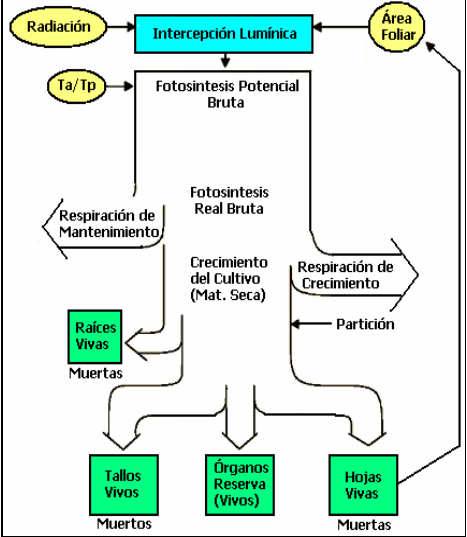
\includegraphics[scale=0.8]{Images/proceso_de_crecimiento_del_cultivo_wofost.png}
	\caption{Procesos del crecimiento del cultivo en WOFOST \parencite{sebem2005aportaciones}}
	\label{fig:img_3}
\end{figure}

La materia seca producida en cada uno de los órganos se calcula en función de la total, aplicando factores que son función del estadio de desarrollo fenológico del cultivo. La curva de crecimiento del cultivo se obtiene integrando el incremento diario de materia seca, para cada uno de los distintos órganos.\\

Los procesos que son simulados en el sistema pueden reagruparse en:

\begin{enumerate}
	\item Simulación del desarrollo fenológico del cultivo. En todo sistema de simulación es esencial determinar los distintos estados fenológicos de la planta, pues, dependiendo de éstos, los procesos fisiológicos y morfológicos son distintos. El más importante es el cambio entre estado vegetativo y reproductor, pues determina la transformación más significativa de reparto de la materia seca en los distintos órganos. Un cultivo pasar por sucesivos estadios fenológicos, la duración dependerá de la tasa de desarrollo. Los principales estadios fenológicos en cultivos anuales son:
	\begin{itemize}
		\item Fecha de siembra. Puede ser conocida o en su defecto calculada por el modelo. 
		\item Nascencia. Viene caracterizada por la aparición de la parte aérea del cultivo aunque lo normal es que la simulación comience en la nascencia, si se quiere proceder a la simulación desde la fecha de siembra, la fecha de nascencia puede calcularse mediante la suma de temperaturas efectivas (temperaturas comprendidas entre dos límites entre los cuales tienen lugar los procesos fenológicos) a partir de la fecha de siembra.
		\item Floración. Es la etapa en que las glumillas de la flor empiezan a separarse.
		\item Maduración. Se produce cuando los órganos de reserva han alcanzado una composición adecuada para su consumo y conservación. 
	\end{itemize}
	La duración de los distintos estadios es función de la tasa de desarrollo. En el modelo, la tasa de desarrollo antes de la floración está controlada por la temperatura y la longitud del día mientras que después de la floración únicamente está regulada por la temperatura. Temperaturas más altas acortan los periodos de crecimiento ya que la tasa de desarrollo es mayor.
	
	En WOFOST la fenología se describe mediante una variable de estado sin dimensión (D); para la mayoría de los cultivos anuales se considera 0 en la emergencia, 1 en la floración y 2 en la madurez. 
	
	Para determinar el efecto de la temperatura en el estado de desarrollo se emplea el concepto de tiempo termal, definido como la suma de temperaturas o suma de calor. El tiempo termal es la integración en el tiempo de temperaturas diarias efectivas después de la emergencia. La temperatura efectiva es la diferencia entre la temperatura media diaria y una temperatura base por debajo de la cual se considera que no hay desarrollo, esta temperatura efectiva no puede ser negativa ni superior a un máximo incremento diario. El estado fenológico se calcula dividiendo el tiempo termal requerido para pasar de un estado de desarrollo al siguiente. Para calcular el tiempo entre la siembra y la emergencia del cultivo WOFOST utiliza otras variables de tiempo termales.
	
	En algunos cultivos el desarrollo fenológico se ve influido también por el fotoperíodo. Este fenómeno es considerado en WOFOST como un factor de reducción (valor entre 0 y 1) para la tasa de desarrollo hasta floración basado en un fotoperíodo óptimo y crítico.
	
	El estado de desarrollo determina, entre otras cosas, la partición de los asimilados entre los distintos órganos (hojas, tallos, raíces y órganos de reserva). Después de la germinación la mayoría de los asimilados se convierten en tejido foliar o radicular y posteriormente en tallo. La partición en tejido radicular disminuye gradualmente llegando a cero cuando el desarrollo es 1 (floración). A partir de la floración los órganos de reserva reciben la mayor parte de los asimilados disponibles. 
	
	En los cálculos, se asigna primero una fracción de los asimilados a las raíces, el resto se divide entre los órganos por encima del suelo. Para iniciar la simulación se debe conocer el peso seco y el índice de área foliar en la emergencia. Desde el principio del crecimiento del cultivo, la reserva de asimilados en las hojas determina el incremento del índice foliar, calculado multiplicando el peso de la materia seca de las hojas por el área foliar específica. Sin embargo la expansión del área foliar puede verse limitada por el incremento máximo diario en el índice de área foliar que depende de la temperatura. El aumento del área foliar conlleva una mayor intercepción de la luz y, por tanto, una mayor tasa de crecimiento potencial. Esto se traduce en un crecimiento exponencial que dura hasta que toda la luz es interceptada (LAI>=3). Seguidamente el crecimiento es constante hasta que el área foliar y su capacidad de fotosíntesis disminuye debido a la senescencia del cultivo. 
	
	\item  La producción diaria de materia seca. Se estima mediante el cálculo de la tasa bruta de asimilación de $ CO_2 $ total diaria y la asimilación bruta de $ CO_2 $ total instantánea con base diaria. La primera puede ser calculada integrando la asimilación de $ CO_2 $ bruta total instantánea con base diaria. La asimilación se origina por la luz interceptada, de modo que esta integración sólo es necesaria si se produce asimilación instantánea, por ejemplo, si no existe superficie foliar no hay luz interceptada y no hay fotosíntesis.
	
	\item La asimilación real de $ CO_2 $. Se obtiene a partir de la asimilación bruta de $ CO_2 $ al tener en consideración el gasto de $ CO_2 $ debido principalmente a la respiración de mantenimiento, respiración de crecimiento y a reparto de la materia seca. 
	
	Parte de los hidratos de carbono producidos se respiran para mantener las estructuras, este proceso puede consumir del 15 al 30\% de los carbohidratos producidos durante el ciclo del cultivo con lo que resulta importante cuantificar con precisión este proceso. La planta también consume los compuestos de carbono sintetizados durante la fotosíntesis en su propio crecimiento. Los asimilados se reparten en la planta según el estado fenológico y los distintos órganos, la tasa de la materia seca total del cultivo puede considerarse como:
	\begin{align*}
		&\Delta W = C_e R_g\\
		&\text{donde: } \\
		&\Delta W  \Rightarrow \text{ tasa de crecimiento de la materia seca total del cultivo [$ kg \; ha^{-1} \; d^{-1} $] } \\
		&C_e  \Rightarrow \text{ factor de eficiencia de la conversión de asimilados [$ kg \; kg^{-1} $] } \\
		&R_g \Rightarrow \text{tasa de respiración de crecimiento [$ kg \; ha^{-1} \; d^{-1} $] } \\
		&\text{donde $ C_e $ se define como: } \\ 
		&C_e = \frac{1}{\sum_{i=1}^{i=2}\frac{pc_i}{C_{e,i}}(1-pc_{rt})+\frac{pc_{rt}}{C_{e,rt}} } \\
		&\text{donde: } \\
		& C_{e,i}  \Rightarrow \text{ factor de eficiencia de conversión de los asimilados de un órgano específico [$ kg \; kg^{-1} $] } \\
		& pc_i  \Rightarrow \text{ factor de partición del órgano $ i $ [$ kg \; kg^{-1} $] } \\
		& i \Rightarrow \text{ hojas (lv), órganos de reserva(so), tallos (st) } \\
		& rt \Rightarrow \text{raíces}
	\end{align*}
	
	Para poder hacer funcionar el modelo son necesarios, para cada cultivo, una numerosa serie de parámetros que se determinan empíricamente, por ejemplo para estimar la fecha de emergencia es necesario conocer la suma de temperaturas medias diarias (TSUMEN) que se considera estiman el tiempo transcurrido entre la siembra y la nascencia del cultivo, estas temperaturas medias deben superar una temperatura base (TBASEM) y sin sobrepasar un incremento máximo diario (TEFFMX). 
	
\end{enumerate}


\subsection{Sub-modelo de Agua en el Suelo \parencite{sebem2005aportaciones}}

Es importante para un modelo de simulación tener en cuenta el balance hídrico para conocer si un cultivo está sujeto a estrés. Su objetivo será calcular diariamente la cantidad real de agua del suelo para que determinar el agua disponible para el cultivo y su transpiración. La simulación de las variables biológicas (rendimiento de los órganos de almacenamiento y biomasa total) se ha realizado para condiciones sin limitación de agua y considerándola factor limitante. 

Para el cálculo de los flujos de agua se requiere conocer los parámetros de pluviosidad, superficie de almacenamiento, superficie de escorrentía, evaporación de la superficie del suelo, transpiración del cultivo, percolación de la zona de enraizamiento a horizontes más profundos y ascensión capilar a la zona de raíces. 

El contenido real del agua en el suelo puede estimarse mediante la ecuación:
\begin{align*}
	&\theta_t = \frac{IN_{up}+(IN_{low}-T_a)}{RD}\Delta t \\
	&\text{donde: } \\
	&IN_{up}=P+I_e-E_s+SS_t/\Delta t - SR \\
	&IN_{low}=CR-Perc \\
	&\text{donde: } \\
	&\Theta_t  \Rightarrow \text{ contenido en agua real de la zona de las raíces en el intervalo de tiempo [$ cm^3 \; cm^{-3} $] } \\
	&IN_{up} \Rightarrow \text{ tasa de afluencia neta a través del límite superior de la zona radicular [$ cm \; d^{-1} $]} \\
	&IN_{low} \Rightarrow \text{ tasa de afluencia neta a través del límite inferior de la zona radicular [$ cm \; d^{-1} $]} \\
	&T_a \Rightarrow \text{ tasa de transpiración real del cultivo [$ cm \; d^{-1} $]} \\
	&RD \Rightarrow \text{ profundidad real de enraizamiento  [$ cm $]} \\
	&P \Rightarrow \text{ intensidad de la precipitación  [$ cm \; d^{-1} $]} \\
	&I_e \Rightarrow \text{ irrigación diaria efectiva  [$ cm \; d^{-1} $]} \\
	&E_s \Rightarrow \text{ tasa de evaporación del suelo [$ cm \; d^{-1} $]} \\
	&SS_t \Rightarrow \text{ superficie de almacenamiento [$ cm $]} \\
	&SR \Rightarrow \text{ tasa de escorrentía [$ cm \; d^{-1} $]} \\
	&CR \Rightarrow \text{ tasa de ascenso capilar [$ cm \; d^{-1} $]} \\
	&Perc \Rightarrow \text{ tasa de percolación [$ cm \; d^{-1} $]} \\
	&\delta t \Rightarrow \text{ intervalo de tiempo [$ d $]} \\
	&Z_t \Rightarrow \text{ profundidad de la capa freática [$ cm $]} \\
\end{align*}

Los procesos que afectan directamente al contenido en agua del suelo radicular (figura \ref{fig:img_4}) son:
\begin{enumerate}
	\item Infiltración : paso del agua de la superficie del suelo a la zona radicular.
	\item Evaporación : pérdida de agua del suelo a la atmósfera.
	\item Transpiración : pérdida de agua.
	\item Percolación : transporte hacia abajo del agua de la zona radicular a la zona inferior a ésta.
	\item Ascensión capilar : transporte hacia la zona radicular.
\end{enumerate}

\begin{figure}[!h]
	\centering
	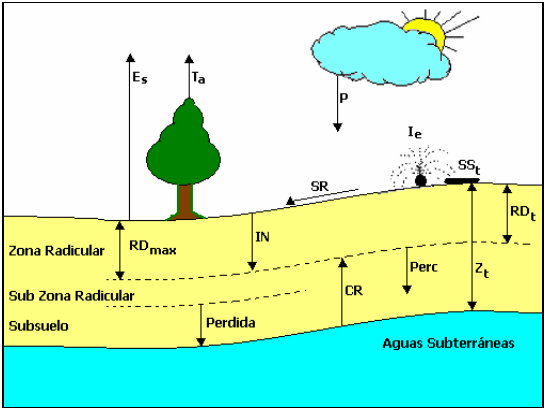
\includegraphics[scale=0.8]{Images/representacion_esquematica_de_los_componentes_del_balance_del_agua_suelo.png}
	\caption{- Representación esquemática de los componentes del balance de agua del suelo. \parencite{sebem2005aportaciones}}
	\label{fig:img_4}
\end{figure}

El contenido en agua de la zona radicular se obtiene a partir del cálculo diario del balance hídrico. En WOFOST se distinguen tres diferentes submodelos de agua en el suelo. Aunque WOFOST admite tres tipos de cálculos distintos del balance hídrico, el WOFOST de CGMS sólo considera los dos primeros sub-modelos, el tercero no es operativo por no disponer al pF (potencial capilar) del suelo.
\begin{enumerate}
	\item Cálculo del balance hídrico del suelo para la producción potencial: El más simple de los balances se aplica para simular la producción potencial. Se considera que la planta crece sin estrés hídrico asumiendo que el suelo está permanentemente a capacidad de campo, de modo que:
	\begin{align*}
		&\theta_t=\theta_{fc} \\
		&\text{donde: } \\
		&\theta_t  \Rightarrow \text{ contenido real del agua del suelo [$ cm^3 \; cm^{-3} $] } \\
		&\theta_{fc}  \Rightarrow \text{ contenido a capacidad del campo [$ cm^3 |; cm^{-3} $] } \\
	\end{align*}
	En los cálculos no se tienen en cuenta la precipitación, irrigación, ascensión capilar y el drenaje, aunque estos procesos puedan ocurrir. Los únicos dos procesos que se consideran son la transpiración del cultivo y evaporación del suelo.
	
	La tasa de evaporación para la mayoría de los cultivos (cultivos sin conductos de aire en las raíces y que no soportan el encharcamiento) se calcula como la tasa de evaporación de la superficie del suelo:
	\begin{align*}
		&E_s=E_{s,max}\frac{\theta_{fc}-\frac{\theta_{wp}}{3}}{\theta_{max}-\frac{\theta_{wp}}{3}} \\
		&\text{donde: } \\
		&E_s  \Rightarrow \text{ tasa de evaporación de la superficie de suelo sombreada [$ cm \; d^{-1} $] } \\
		&E_{s,max}  \Rightarrow \text{ tasa de evaporación máxima de la superficie de suelo sombreada [$ cm \; d^{-1} $] } \\
		&\theta_{wp}  \Rightarrow \text{ contenido en agua en el punto de marchites [$ cm^3 \; cm^{-3} $] } \\
		&\theta_{max}  \Rightarrow \text{ porosidad del suelo [$ cm^3 \; cm^{-3} $] } \\
		&\text{Calculándose la máxima tasa de evaporación de la superficie de suelo sombreado como: } \\
		&E_{s,max}=EO_se^{-k_{gb}LAI} \\
		&\text{donde: } \\
		&EO_s  \Rightarrow \text{ tasa de evaporación potencial de la superficie de un suelo desnudo [$ cm \; d^{-1} $] } \\
		&k_{gb}  \Rightarrow \text{ coeficiente de extinción para la radiación global total [$ - $] } \\
		&LAI  \Rightarrow \text{ índice de área foliar [$ ha \; ha^{-1} $] } \\
	\end{align*}
	\item Cálculo del balance hídrico del suelo cuando no se considera la capa freática: El segundo sub-modelo para la situación de producción con limitaciones de agua se aplica a un suelo que drena libremente, la capa freática es tan profunda que no influye en el contenido de agua de la zona radicular. 
	
	Para la zona de enraizamiento se calcula diariamente la ecuación del balance hídrico. El balance hídrico es impulsado por la precipitación y la evapotranspiración. Los procesos considerados son la infiltración, retención de agua en el suelo, percolación y pérdida de agua por debajo de la zona radicular máxima. El agua puede retenerse en el suelo hasta el contenido de la capacidad de campo. Se distinguen en el suelo tres zonas:
	\begin{enumerate}
		\item zona de enraizamiento, entre la superficie y la profundidad real de las raíces.
		\item zona inferior, entre la profundidad real de enraizamiento y la máxima.
		\item subsuelo, por debajo de la profundidad máxima.
	\end{enumerate}
	\item Cálculo del balance hídrico del suelo cuando se considera la capa freática: El tercer sub-modelo se aplica para calcular la producción con limitación de agua en suelos que tienen la influencia de una capa freática poco profunda en la zona radicular. La diferencia con respecto al segundo submodelo es que la capacidad de retención del agua en el suelo está determinada por la profundidad de la capa freática, es decir, la tasa de percolación.
	
	Aunque las simulaciones se llevan a cabo mediante CGMS también se ha utilizado el modelo de simulación WOFOST 7.1 con la utilidad WCC (WOFOST Control Centre 1.5). WCC facilita la selección de los ficheros correspondientes al clima, cultivos y suelo así como el tratamiento y visualización de los datos resultantes de la simulación. 
	
	Existe la opción de realizar varias simulaciones a la vez (rerun) cambiando algunos de los parámetros con el objeto de estudiar el cambio de las variables simuladas. 
	
	Mediante WOFOST se pueden obtener distintos tipos de resultados: 
	\begin{enumerate}
		\item \textbf{Potenciales}. Producción potencial del cultivo: (IDSEM) Número de días desde la nascencia (d); (DVS) Estado de desarrollo del cultivo (-); (TSUM) Tiempo térmico desde la nascencia (ºC d); (WLV) Peso seco de las hojas vivas (k ha); (WST) Peso seco de los tallos vivos (k ha); (WSO) Peso seco de los órganos de reserva vivos (k ha); (TAGP) Producción total sobre el suelo (órganos vivos y muertos) (k ha); (LAI) Índice de Área Foliar (área foliar/superficie del suelo) (ha/ha); (TRA) Tasa de transpiración (mm/d); (GASS) Tasa de asimilación bruta (mm/d); (MRES) Tasa de respiración de mantenimiento (mm/d); (DMI) Incremento de la tasa de materia seca (k/ha d). 
		\item\textbf{ Con limitación de agua}. Producción con limitación de agua: (WLV) Peso seco de las hojas vivas (k ha); (WST) Peso seco de las tallos vivas (k ha); (WSO) Peso seco de las órganos de reserva vivos (k ha); (TAGP) Producción total sobre el suelo (órganos vivos y muertos) (k ha); (LAI) Índice de Área Foliar (área foliar/superficie del suelo) (ha/ha), (RD) Profundidad de la zona de enraizamiento real (cm); (SM) Contenido de agua en el suelo en la zona de enraizamiento real (cm3 agua/cm3 suelo); (RESRV) Agua del suelo disponible en la zona de enraizamiento potencial (en y por debajo de la zona de enraizamiento real) (cm suelo); (AVAIL) Agua disponible en la zona de enraizamiento real (cm agua) Sólo cuando se simula sin la influencia de agua subterránea); (RAIN) Precipitación total en el período de simulación (mm); (TRA) Tasa de transpiración (mm/d); (EVA(P)) Tasa de evaporación desde el suelo o del agua almacenada en la superficie del suelo (mm/d); (SS) Superficie de almacenamiento (cm agua); (ZT) Profundidad de la capa freática (cm por debajo de la superficie del suelo); (wet) Días caracterizados por un crecimiento reducido debido a la falta de oxígeno (d); (dry) Días caracterizados por un crecimiento reducido debido a la falta de agua (d). 
		\item\textbf{ Con limitación de nutrientes}. Producción con limitación de nutrientes: Este caso no va a ser considerado en los procesos de simulación que van a llevarse a cabo ya que no se dispone de los datos. 
		\item\textbf{ Balance hídrico}. Los resultados de balance hídrico se obtienen tanto para todo el sistema como para la zona radicular. Para todo el sistema los resultados que obtenemos son: (1) Contenido de agua inicial y final y su diferencia (bien para la zona radicular máxima o para los 10 primeros cm cuando consideramos la influencia del agua del suelo); (2) Superficie de almacenamiento de agua inicial y final y su diferencia; (3) Precipitación; (4) Evaporación (del suelo o la superficie de agua) y transpiración (del cultivo); juntos son pérdida de agua a la atmósfera y (5) Agua de escorrentía, percolación al agua del terreno y pérdida de agua debida al drenaje (cuando hay agua freática).
		
		Los resultados del balance hídrico en la zona radicular comprende los siguientes datos: (1) Contenido de agua inicial y final y su diferencia en la zona radicular; (2) Infiltración a la zona radicular (ejemplo, precipitación menos escorrentía); (3) Evaporación (del suelo) y transpiración (del cultivo); (4) Incremento del agua disponible debido al crecimiento radicular; (5) Percolación al agua del suelo y (6) Aumento de la capilaridad (cuando existe agua freática).
		
		\item Resultados resumidos: WCC resume en un fichero las variables de salida para los distintos años, así como los datos estadísticos (media, desviación típica y coeficiente de variación) de todos los años.
	\end{enumerate}
\end{enumerate}

Luego de analizar todo lo anteriormente expuesto, se puede llegar a la conclusión que las principales razones por las que se escogió WOFOST como modelo para desarrollar la presente investigación son, en primer lugar, este modelo permite el estudio del comportamiento del cultivo y su rendimiento bajo diversas condiciones del medio, esto es de gran utilidad en Cuba ya que el país posee gran diversidad en los suelos, en las temperaturas, en las condiciones hídricas y otros factores que pueden influenciar el desarrollo de un determinado cultivo. En variadas ocasiones en Cuba hay limitantes hídricas, siendo WOFOST una de las mejores soluciones para estimar variables biológicas como el rendimiento de los órganos de almacenamiento y la biomasa total en dichas condiciones. Además brinda la posibilidad de analizar por separado el crecimiento del cultivo y el balance del agua, ya que el modelo se divide en dos submodelos. Este modelo mecanicista y dinámico ha sido aplicado en todo el mundo en cultivos en una amplia gama de condiciones climáticas y de gestión. Considera las limitantes de nitrógeno, fósforo y potasio en el crecimiento vegetal, aunque no considera los efectos tóxicos del alto contenido salino y/o de aluminio del suelo, aunque la mayoría de los modelos actuales no lo hacen.

\section{Tecnología y Herramientas a Usar}

Cuando se decidió escoger el modelo WOFOST para ser utilizado en la tesis, se decidió también buscar tecnologías viables para poder desarrollar el resto del proyecto.\\

Luego de una ardua búsqueda se encontró una implementación de este modelo, \textbf{PCSE} (Python Crop Simulation Environment)  “Entorno de simulación de cultivos en Python”, que según su página oficial \parencite{wofost_oficial_page} , se desarrolló debido a la necesidad de reimplementar los modelos de simulación de cultivos que se desarrollaron en Wageningen. Muchos de los modelos de simulación de cultivos de Wageningen se desarrollaron originalmente en FORTRAN77 o utilizando el FORTRAN Simulation Translator (FST). Aunque este enfoque ha dado lugar a modelos de gran calidad y con un alto rendimiento numérico, las limitaciones inherentes a los modelos escritos en FORTRAN son cada vez más evidentes:
\begin{itemize}
	\item La estructura de los modelos suele ser bastante monolítica y las diferentes partes están muy acopladas. Sustituir partes del modelo por otro enfoque de simulación no es fácil.
	\item Los modelos se basan en la I/O basada en archivos, que es difícil de cambiar. Por ejemplo, la interconexión con las bases de datos es complicada en FORTRAN.
	\item En general, con lenguajes de bajo nivel como FORTRAN, las cosas sencillas ya requieren muchas líneas de código y es fácil que se cometan errores, sobre todo por parte de agrónomos y científicos de cultivos que tienen poca experiencia en el desarrollo o la adaptación de software.
\end{itemize}

Para superar muchas de las limitaciones anteriores, se creó el Entorno de Simulación de Cultivos Python (PCSE). Este proporciona un entorno para desarrollar modelos de simulación, así como una serie de implementaciones de modelos de simulación de cultivos. PCSE está escrito en código Python puro, lo que lo hace más flexible, más fácil de modificar y extensible, permitiendo una fácil interconexión con bases de datos, interfaces gráficas de usuario, herramientas de visualización y paquetes numéricos/estadísticos. PCSE tiene varias características interesantes:

\begin{itemize}
	\item Implementación en Python puro. El núcleo del sistema tiene un pequeño número de dependencias fuera de la biblioteca estándar de Python. Sin embargo, muchos proveedores de datos requieren la instalación de ciertos paquetes. La mayoría de ellos pueden ser instalados automáticamente desde el Python Package Index (PyPI) (SQLAlchemy, PyYAML, xlrd, openpyxl, requests) y en el procesamiento de la salida de los modelos se hace más fácilmente con pandas DataFrames.
	\item Diseño modular que permite añadir o cambiar componentes con relativa rapidez con un enfoque sencillo pero potente para comunicar variables entre módulos.
	\item Al igual que el FST, impone un buen diseño del modelo al separar explícitamente los parámetros, las variables de tasa y las variables de estado. Además, PCSE se encarga de la inicialización del módulo, el cálculo de las tasas de cambio, la actualización de las variables de estado y las acciones necesarias para finalizar la simulación.
	\item La Input/Output está completamente separada del propio modelo de simulación. Por lo tanto, los modelos PCSE pueden leer y escribir fácilmente en archivos de texto, bases de datos y formatos científicos como HDF o NetCDF. Además, los modelos PCSE se pueden incrustar fácilmente en, por ejemplo, contenedores Docker para construir una API web alrededor de un modelo de cultivo.
	\item Pruebas integradas de los módulos del programa que garantizan la integridad del sistema.
\end{itemize}

PCSE se desarrolló ante todo por una necesidad científica, para poder adaptar rápidamente los modelos y probar las ideas. En el ámbito científico, Python se está convirtiendo rápidamente en una herramienta para la implementación de algoritmos, la visualización y el análisis exploratorio debido a su sintaxis clara y su facilidad de uso. Una ventaja adicional es que la implementación en C de Python puede interconectarse fácilmente con rutinas escritas en FORTRAN y, por tanto, muchas rutinas FORTRAN pueden ser reutilizadas por modelos de simulación escritos con PCSE.

Existen muchos paquetes para el análisis numérico (por ejemplo, NumPy, SciPy), la visualización (por ejemplo, MatPlotLib, Chaco), la computación distribuida (por ejemplo, IPython, pyMPI) y la interconexión con bases de datos (por ejemplo, SQLAlchemy). Además, para los análisis estadísticos se puede establecer una interfaz con el  R-project a través de Rpy o Rserve. Por último, Python es un lenguaje de programación interpretado de código abierto que se ejecuta en casi cualquier hardware y sistema operativo.

Dadas las consideraciones anteriores, se reconoció rápidamente que Python era una buena opción. Aunque, PCSE fue desarrollado para fines científicos, ya ha sido implementado para tareas en entornos de producción y ha sido incrustado en servicios web basados en contenedores.\\

Hasta la versión 4.1, PCSE se denominaba "PyWOFOST", ya que su objetivo principal era proporcionar una implementación en Python del modelo de simulación de cultivos WOFOST. Sin embargo, a medida que el sistema ha ido creciendo, se ha hecho evidente que puede utilizarse para implementar, ampliar o hibridar modelos de simulación (de cultivos). Por lo tanto, el nombre "PyWOFOST" se volvió demasiado estrecho y se seleccionó el nombre de Entorno de Simulación de Cultivos Python en analogía con el Entorno de Simulación FORTRAN (FSE).\\

El PCSE también tiene sus limitaciones, entre estas se puede citar la velocidad, la flexibilidad tiene un precio; PCSE es considerablemente más lento que los modelos equivalentes escritos en FORTRAN u otro lenguaje compilado. El enfoque de simulación en PCSE se limita actualmente a la integración rectangular (Euler) con un paso de tiempo diario fijo. Sin embargo, el paso de tiempo interno de los módulos puede ser más preciso si es necesario. Además, no hay interfaz gráfica de usuario. Sin embargo, la falta de una interfaz de usuario se compensa en parte mediante el uso de PCSE con el paquete pandas y el cuaderno Jupyter. La salida de PCSE se puede convertir fácilmente en un DataFrame de pandas que se puede utilizar para mostrar gráficos en un cuaderno Jupyter.\\

Entre la amplia cantidad de librerías encontradas en Python para diversos usos, se cuenta con Flask, que según  \parencite{flask_que_2017}, es un micro Framework para desarrollar una App básica o una forma ágil, o sea, para determinadas aplicaciones que no necesiten de muchas extenciones; incluye un servidor web de desarrollo, por lo que no se necesita de una infraestructura con un servidor web para probar las aplicaciones, en otras palabras, tiene hot-reload; tiene un depurador y soporte integrado para pruebas unitarias; es compatible con Python3 y con wsgi, que no es más que un protocolo que utilizan los servidores web para servir páginas web escritas en Python; tiene un fácil manejo de rutas; soporta de manera nativa el uso de cookies seguras; se pueden usar sesiones; es Open Source y se encuentra amparado bajo una licencia BSD; presenta buena documentación con ejemplos de proyectos en GitHub; sirve para construir servicios web como aplicaciones de contenido estático o APIs REST, que es precisamente la tecnología que se desea usar, por lo que se detallará más a continuación.\\

Una \textbf{API} \parencite{apirest_definicion_2020} (Application Programming Interface)  “Interfaz del programa de aplicación” es un conjunto de reglas que permite que diferentes programas se comuniquen entre sí. Describe la manera apropiada para que un desarrollador de software componga un programa en un servidor que se comunica con varias aplicaciones cliente.

La integración de API se refiere a un par de aplicaciones (dos o más) interconectadas a través de sus API para intercambiar datos y realizar una función conjunta, lo que permite la interacción entre aplicaciones.

Ahora que hemos definido la API, pasemos a las API REST. Varios sitios web como Amazon, Google, Facebook, LinkedIn y Twitter utilizan API basadas en REST que permiten a los usuarios comunicarse con estos servicios en la nube. Esta se ajusta a los límites de la arquitectura REST y permite la interacción con los servicios web de RESTful.\\

Como se ha mencionado anteriormente la integración de API se refiere a dos o más aplicaciones interconectadas, de manera que si se tuviese una aplicación servidor encargada de ejecutar pedidos, y brindar información, a pesar de su eficacia, esta no es muy intuitiva para los usuarios, por lo tanto, una forma de que el usuario final pueda interactuar con el servidor backend sería mediante una interfaz de usuario, ya sea una aplicación de escritorio, móvil o una página web, que es una de las ideas finales de este proyecto, hacer llegar este tipo de aplicación a usuarios inexpertos en el tema de la modelación y simulación, dejando sólo que se concentren en interactuar de manera sencilla con la simulación de cultivos sin necesidad de escribir una línea de código.\\

Para el desarrollo de la interfaz de usuario el autor propone la creación de una página web utilizando React como tecnología principal. Según su página oficial \parencite{react_oficial_page}, React se define como una biblioteca de javaScript para construir interfaces de usuario. 

React permite además crear interfaces de usuario interactivas de forma sencilla; crear componentes encapsulados que manejen su propio estado, y convertirlos en interfaces de usuario complejas; renderizar desde el servidor usando Node, así como potencializar aplicaciones móviles usando React Native. Además, React se encarga de actualizar y renderizar de manera eficiente los componentes correctos en una aplicación cuando los datos cambien; las vistas declarativas hacen que el código sea más predecible, por lo tanto, fácil de depurar; dado que la lógica de los componentes está escrita en JavaScript y no en plantillas, es posible pasar datos de forma sencilla a través de la aplicación y mantener el estado fuera del DOM. React se vincula al resto de herramientas tecnológicas, así que será posible desarrollar nuevas características sin necesidad de volver a escribir el código existente.\\

Solo falta mencionar, donde almacenar toda la información, configuración, variables de entrada de cultivos, suelo y clima. Para esto se usará, una base de datos SQLite, que según su página oficial \parencite{sqlite_nodate}, es una biblioteca en lenguaje C que implementa un motor de base de datos SQL pequeño, rápido, autónomo, de alta fiabilidad y con todas las funciones; es el motor de base de datos más utilizado en el mundo; está integrado en todos los teléfonos móviles y en la mayoría de los ordenadores, y viene incluido en innumerables aplicaciones que la gente utiliza a diario; su formato de archivo es estable, multiplataforma y compatible con versiones anteriores, y los desarrolladores se comprometen a mantenerlo hasta el año 2050; los archivos de bases de datos SQLite se utilizan habitualmente como contenedores para transferir contenidos ricos entre sistemas y como formato de archivo de datos a largo plazo; hay más de 1 billón (1e12) de bases de datos SQLite en uso activo. Su código fuente es de dominio público y su uso es gratuito para todo el mundo.\\













\chapter{Detalles de Implementación y Experimentos}\label{chapter:implementation}

Para una mejor comprensión de este capítulo, el autor estima conveniente dividirlo en los siguientes sub-capítulos:
\begin{itemize}
	\item Estructura y detalles del proyecto en general (\ref{chapter:implementation:estructure}).
	\item Instalación, implementación y utilización del modelo WOFOST mediante el Entorno de simulación de cultivos en Python (PCSE) (\ref{chapter:implementation:wofost}).
	\item Implementación de un servidor flask backend (API) para el manejo del entorno de simulación de forma aislada a la interfaz de usuario (\ref{chapter:implementation:backend}).
	\item Tutorial e implementación de la interfaz de usuario (frontend) (\ref{chapter:implementation:frontend}).
	\item Experimentación y exposición de resultados finales (\ref{chapter:implementation:results}).
\end{itemize}

\section{Estructura y detalles del proyecto en general}\label{chapter:implementation:estructure}
El proyecto se creó para alojarse en servidores Internet con una arquitectura REST, donde lo ideal sería la obtención de un host donde alojar el API server y el frontend, de forma tal que no sea el cliente final quien tenga que cargar con el peso de la simulación en su ordenador, teléfono, tablet u otra fuente de acceso; por lo que este sólo se tendría que preocupar por tener conexión a Internet y un dispositivo donde poder interactuar con la aplicación.

Internet es un medio fundamental en el proyecto dado que este, además de alojare en servidores en la nube, requiere de Internet para poder realizar acciones como la geo-localización, carga de datos climáticos, carga de datos de cultivos, suelo, entre otros. Aún suponiendo que el proyecto corriera en alguna maquina local donde coexistieran frontend y backend (no se menciona db dado que esta es SQLite y puede alojarse donde mismo el backend), es necesario contar con conexión a Internet, para la comunicación con las APIs de datos mencionadas anteriormente.\\

La aplicación tiene una arquitectura REST, contando con un servidor backend y otro frontend escritos en tecnologías completamente diferentes. Para el primero se usó Python como lenguaje de programación, usando el micro-framework flask-restful. La interfaz de usuario, se escribió usando como framework React y TypeScript para una mayor riqueza de implementación gracias a su tipado fuerte.\\

\subsection{Estructura de directorios y archivos del backend}
El servidor backend comienza en el directorio raíz \lstinline|CropSimulatorWeb/Backend|, más específico, en \lstinline|CropSimulatorWeb/Backend/src/app|.

\begin{figure}[!h]
	\centering
	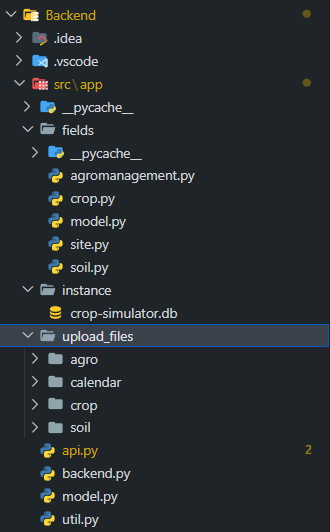
\includegraphics[width=0.4\linewidth]{Images/back-structure}
	\caption{Estructura del Backend}
	\label{fig:back-structure}
\end{figure}

En el directorio raíz tenemos el directorio \lstinline|fields|, el cual contiene archivos que se encargan de controlar la estructura de cada modelo al salir de la base de datos mediante el decorador \lstinline|@marshal_with|, así como un conjunto de funciones para el manejo y limpieza de estos modelos, para leer archivos guardados en el servidor en el directorio \lstinline|upload_files|, entre otras funcionalidades.

El directorio \lstinline|instance| guarda el archivo de base de datos SQLite.

En \lstinline|upload_files| se encuentran todos los archivos subidos al servidor, este se particiona en: \lstinline|agro|, \lstinline|calendar|, \lstinline|crop|, \lstinline|soil|. Cada uno de estos tiene un formato específico, ya sea \lstinline|YAML| o \lstinline|CABO|.

Luego se tienen los archivos siguientes:
\begin{itemize}
	\item En \lstinline|util.py| se tienen las funciones para parsear de Yaml a un diccionario en Python y viceversa.
	\item En \lstinline|model.py| se encuentra la clase \lstinline|WofostModel| que no es más que una clase wrapper de los modelos \lstinline|Wofost71_WLP_FD, Wofost71_PP y Wofost72_Phenology | contenidos en \lstinline|pcse.models|, encargada de instanciar estos con un conjunto de parámetros iniciales, así como de proveer funciones para el manejo de su simulación dentro de un ambiente previamente creado.
	\item \lstinline|backend.py| es el encargado de crear la instancia de \lstinline|Flask| y \lstinline|Api|, algunas variables de configuración inicial como la ruta de \lstinline|uploads|, \lstinline|URL| de la base de datos, crear las tablas correspondientes a esta con los modelos previamente creados, entre otras funcionalidades.
	\item \lstinline|api.py| es el archivo primordial del servidor. Contiene los modelos base de datos per se, funciones para su correcto manejo, enrutadores, requests y responses HTTP (GET, POST, DELETE, PUT) y es el encargado de inicializar toda la aplicación. Una vez ejecutado, se queda a la espera de peticiones de algún proveedor como es el caso de la interfaz de usuario.
\end{itemize}

La estructura antes mencionada se puede apreciar en la (figura \ref{fig:back-structure}). 

\subsection{Estructura de directorios y archivos del frontend}
El servidor frontend comienza en el directorio raíz \lstinline|CropSimulatorWeb/Frontend|.

\begin{figure}[!h]
	\centering
	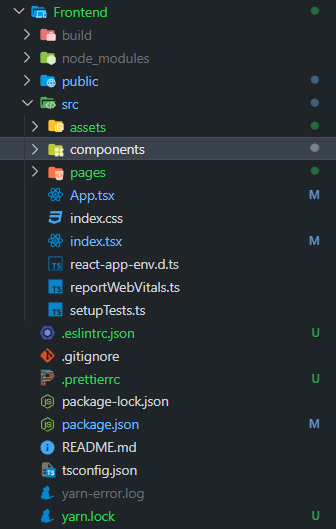
\includegraphics[width=0.4\linewidth]{Images/front-structure-root}
	\caption{Estructura raíz del Frontend}
	\label{fig:front-structure-root}
\end{figure}

Está compuesto por el directorio \lstinline|build|, donde una vez compilada toda la aplicación en desarrollo, se almacena el código listo para lanzar a producción. Luego está \lstinline|node_modules|, que es el directorio encargado de listar los módulos usados en la aplicación.

El directorio \lstinline|public| donde se guardan imágenes, el \lstinline|index.html| central entre otros archivos.

En \lstinline|src| se encuentra todo el código en desarrollo de la aplicación. Está compuesto por \lstinline|assets|, donde se almacenan algunos assets usados como svgs, imágenes, etc; \lstinline|components|, donde se encuentran todos los componentes de la aplicación como el \lstinline|AppBar, Autocomplete, YamlEditor, Drawer|, entre otros; \lstinline|pages|, donde están todas las páginas que componen la aplicación. Entre estas se encuentran: \lstinline|About, Dashboard, Agromanagement, Home, Site, Soil, Crop, DailyWeatherObservations|, etc.

\lstinline|App.tsx| es el componente principal. Es el primero en ser renderizado al iniciar la aplicación; está envuelto en \lstinline|BrowserRouter|, que es el proveedor de las rutas, primero en la jerarquía del DOM.\\

La estructura antes mencionada se puede apreciar en la (figura \ref{fig:front-structure-root}). 

\section{Instalación, implementación y utilización del modelo WOFOST mediante el Entorno de Simulación de Cultivos en Python (PCSE).} \label{chapter:implementation:wofost}

PCSE (Python Crop Simulation Environment) fue desarrollado en Ubuntu 18.04 y Widndows 10 usando Python 3.7 y Python 3.8. Este puede ser usado de igual manera en Windows, Linux o MacOSX. Antes de su instalación se requieren las siguientes dependencias:
\begin{itemize}
	\item \lstinline |SQLAlchemy>=0.8.0|
	\item \lstinline |PyYAML>=3.11|
	\item \lstinline |xlrd>=0.9.3|
	\item \lstinline |openpyxl>=3.0|
	\item \lstinline |requests>=2.0.0|
	\item \lstinline |pandas>=0.20|
	\item \lstinline |traitlets-pcse==5.0.0.dev|
\end{itemize}

PCSE se instala al igual que otra dependencia cualquiera en Python; en el proyecto se usó el gestor de paquetes Python (pip): \lstinline|pip install pcse|.
Una vez instalado, se puede importar de la siguiente manera: \lstinline[alsolanguage=python]|import pcse|. Una forma de probar si su instalación fue correcta es corriendo la función: \lstinline[alsolanguage=python]|pcse.test()|, y se debería obtener en caso positivo una salida parecida a la mostrada en la figura (\ref{fig:pcse-test})

\begin{figure}[!h]
	\centering
	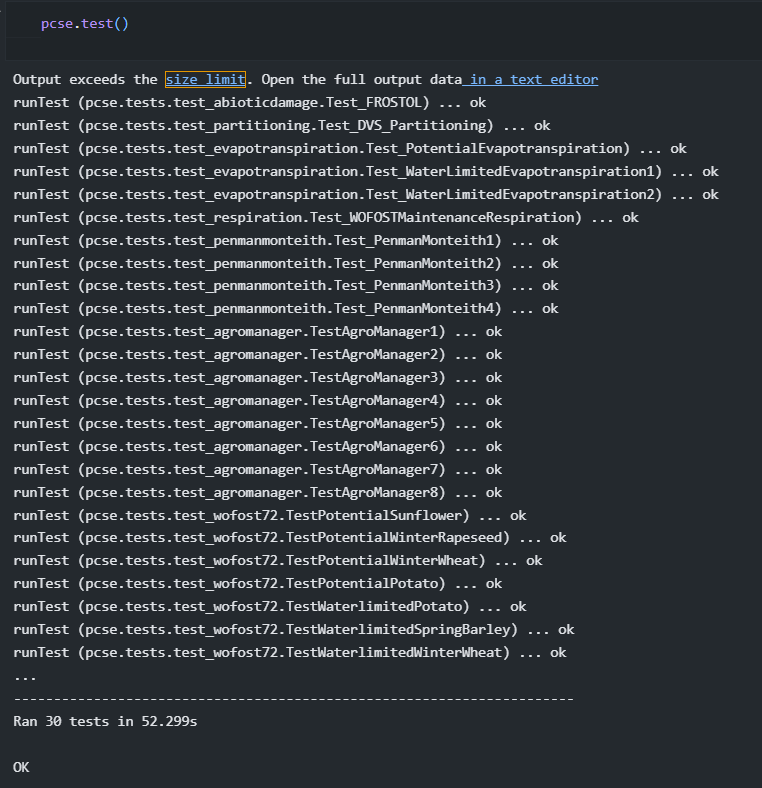
\includegraphics[width=0.4\linewidth]{Images/pcse-test}
	\caption{}
	\label{fig:pcse-test}
\end{figure}

El entorno PCSE, brinda una forma sencilla de trabajar con modelos como ALCEPAS, LINGRA, LINTUL, WOFOST, entre otros. Este último fue el utilizado para el desatollo de la aplicación.

Se puede usar alguno de los modelos de WOFOST (Wofost71\_WLP\_FD (WOFOST7.2 water limited production), Wofost72\_Phenology (WOFOST7.2 phenology only.), Wofost71\_PP (WOFOST7.2 Potential Production), entre otros) importándolo desde \lstinline|pcse.models|, por ejemplo: \lstinline[alsolanguage=python]|from pcse.models import Wofost71_WLP_FD|

Luego se crea una instancia de una de las clases importadas, por ejemplo: \lstinline|Wofost71_WLP_FD| y se inicia pasándole las variables iniciales: \lstinline|parameters, wdp, agromanagement|, es decir:
\lstinline[alsolanguage=python]|wofsim = Wofost71_WLP_FD(parameters, wdp, agromanagement)|

La variable \lstinline|parameters| es una instancia de la clase \lstinline|ParameterProvider| (\lstinline[alsolanguage=python]|from pcse.base import ParameterProvider|), que recibe como argumentos: \lstinline|cropdata, soildata, sitedata|. Un ejemplo de inicialización es:
\lstinline[alsolanguage=python]|parameters = ParameterProvider(cropdata=cropdata, soildata=soildata, sitedata=sitedata)|.\\

Para cargar estos parámetros, se puede hacer de diversas maneras, un ejemplo básico es el siguiente:

\begin{python}
	from pcse.fileinput import CABOFileReader
	cropfile = os.path.join(data_dir, 'sug0601.crop')
	cropdata = CABOFileReader(cropfile)
\end{python}

De igual manera se cargan los parámetros de suelo y sitio:

\begin{python}
	soilfile = os.path.join(data_dir, 'ec3.soil')
	soildata = CABOFileReader(soilfile)
	
	from pcse.util import WOFOST71SiteDataProvider
	sitedata = WOFOST71SiteDataProvider(WAV=100)
\end{python} 

Los parámetros de cultivo (cropdata) consisten en nombres de parámetros y sus valores correspondientes que se necesitan para parametrizar los componentes del modelo de simulación de cultivos. Estos son valores específicos del cultivo con respecto a la fenología, asimilación, respiración, partición de biomasa, etc.
Los parámetros de cultivo para muchos modelos en Wageningen a menudo se proporcionan en el formato CABO; para leer archivos en este formato, \lstinline|CABOFileReader| devuelve un diccionario con pares nombre/valor.

El diccionario de datos del suelo (soildata) proporciona los pares nombre/valor del parámetro relacionados con el tipo de suelo y sus propiedades físicas. El número de estos parámetros varía en dependencia del tipo de balance de agua del suelo usado para la simulación. El ejemplo anterior cargado, de suelo con arena medianamente fina, se suele usar para el balance de agua de suelos de drenaje libre. Este se puede encontrar también en formato CABO.\\

Los parámetros del sitio (sitedata) proporcionan parámetros auxiliares que no están relacionados con el cultivo o el suelo. Algunos ejemplos son las condiciones iniciales del balance hídrico, como el contenido inicial de humedad del suelo (WAV) y el almacenamiento superficial inicial y máximo (SSI, SSMAX). También la concentración atmosférica de $ CO_2 $ es un parámetro típico del sitio. Estos se pueden encontrar en \lstinline|WOFOST71SiteDataProvider| que documenta los parámetros del sitio y proporciona valores predeterminados sensibles.\\

Otro de los parámetros iniciales del modelo es \lstinline|agromanagement|, el cual se encarga de proporcionar la fecha de inicio de la campaña agrícola, fecha de inicio y tipo de inicio de la simulación, así como final y duración máxima. Este último se incluye para evitar simulaciones largas poco realistas, por ejemplo, como resultado de una suma de temperaturas demasiado altas.
El agromanagement se suele definir de una manera diferente, usando sintaxis YAML, permitiendo crear fácilmente estructuras más complejas que se necesitan para definir la gestión agrícola. Este se puede leer mediante la clase \lstinline|YAMLAgroManagementReader| perteneciente a \lstinline|pcse.fileinput|.
Se presenta un ejemplo completo:

\begin{python}
	from pcse.fileinput import YAMLAgroManagementReader
	agromanagement_file = os.path.join(data_dir, 'sugarbeet_calendar.agro')
	agromanagement = YAMLAgroManagementReader(agromanagement_file)
	print(agromanagement)
\end{python}

Donde \lstinline|sugarbeet_calendar.agro| tiene la forma:

\begin{figure}[!h]
	\centering
	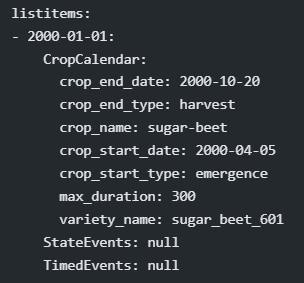
\includegraphics[width=0.4\linewidth]{Images/yaml_agro}
	\caption{}
	\label{fig:yamlagro}
\end{figure}

Como último argumento del modelo, se encuentra \lstinline|weatherdataprovider| abreviado \lstinline|wdp| (Observaciones meteorológicas diarias). Es necesario puesto que se necesitan variables meteorológicas diarias para ejecutar la simulación. Existen varios proveedores en PCSE para leer este tipo de datos. En la aplicación se utilizaron datos de la base de datos NASA Power, que proporciona datos meteorológicos globales con una resolución espacial de 0.5 grados (~50km). Para obtener estos datos se usa la clase \lstinline|NASAPowerWeatherDataProvider| de \lstinline|pcse.db|, la cual requiere latitud y longitud. Esta clase cuenta con su propia caché para velocidad en llamadas posteriores, dado que la primera puede tardar más de 30 segundos. Se muestra a continuación un ejemplo:

\begin{python}
	from pcse.db import NASAPowerWeatherDataProvider
	wdp = NASAPowerWeatherDataProvider(latitude=52, longitude=50)
	print(wdp)
\end{python}

dando como salida:

\begin{figure}[!h]
	\centering
	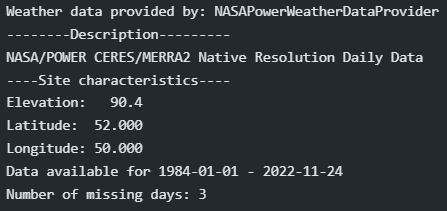
\includegraphics[width=0.4\linewidth]{Images/wdp}
	\caption{}
	\label{fig:wdp}
\end{figure}

Una vez obtenidos todos los anteriores parámetros, se inicializa el modelo de la siguiente forma:

\begin{python}
	from pcse.models import Wofost71_WLP_FD
	wofsim = Wofost71_WLP_FD(parameters, wdp, agromanagement)
\end{python}

Luego de instanciado el modelo, se puede ejecutar una simulación de este $ i $ cantidad de días o ejecutar hasta el final de la campaña.

Para simular $ i $ días se llama el método \lstinline|run| del objeto \lstinline|wofsin| creado, y para mostrar algunos resultados finales, como las fechas de cosecha (DOA, DOH), la biomasa total (TAGP) y el LAI máximo (LAIMAX), se ejecuta la función \lstinline|get_output()|. Por ejemplo:

\begin{python}
	wofsim.run(days)
	output = wofsim.get_output()
	len(output)
\end{python}

Si se quiere simular hasta el final de la campaña, se usa la función \lstinline|run_till_terminate| de \lstinline|wofsin|, por ejemplo:
\begin{python}
	wofsim.run_till_terminate()
\end{python}

\section{Implementación de un servidor Flask backend (API) para el manejo del entorno de simulación de forma aislada a la interfaz de usuario.} \label{chapter:implementation:backend}

La implementación del servidor backend, como se menciona anteriormente, está puramente escrita en Python, facilitando el uso del modelo de simulación WOFOST del pcse.
Dicho server tiene como objetivo crear, actualizar, eliminar, ejecutar y parar entornos de simulación con instancias de modelos WOFOST, datos de suelo, de cultivo, de sitio, de clima, entre otros; y prepararse para ser consumido por una interfaz de usuario o cualquier otra forma de realizar peticiones a este.\\

A continuación se explican las rutas de la api, así como su funcionalidad.
\begin{itemize}
	\item (GET) \lstinline|api/crop|: retorna lista de cultivos almacenados en la db.
	\item (POST) \lstinline|api/crop|: almacena nuevo cultivo en la db. Retorna el cultivo creado. Recibe en el body los datos del cultivo (CRPNAM, TBASEM, TEFFMX, TSUMEM, IDSL, ...)
	\item (GET) \lstinline|api/crop/<int:crop_id>|: retorna el cultivo almacenado en la db cuyo id es igual al pasado en la query.
	\item (DELETE) \lstinline|api/crop/<int:crop_id>|: elimina y retorna el cultivo almacenado en la db cuyo id es igual al pasado en la query.
	\item (PUT) \lstinline|api/crop/<int:crop_id>|: actualiza el cultivo en la db cuyo id es igual al pasado en la query y retorna el cultivo actualizado. Recibe en el body los datos del cultivo (CRPNAM, TBASEM, TEFFMX, TSUMEM, IDSL, ...).
	\item (POST) \lstinline|api/crop/upload|: guarda en el directorio \lstinline|upload_files/crop| un fichero crop (CABO). Recibe en el body el parámetro crop-file de type file.
	
	\item (GET) \lstinline|api/soil|: retorna lista de suelos almacenados en la db.
	\item (POST) \lstinline|api/soil|: almacena nuevo suelo en la db. Retorna el suelo creado. Recibe en el body los datos del suelo (SOLNAM, SMTAB, SMW, SMFCF, SM0, ...)
	\item (GET) \lstinline|api/soil/<int:soil_id>|: retorna el suelo almacenado en la db cuyo id es igual al pasado en la query.
	\item (DELETE) \lstinline|api/soil/<int:soil_id>|: elimina y retorna el suelo almacenado en la db cuyo id es igual al pasado en la query.
	\item (PUT) \lstinline|api/soil/<int:soil_id>|: actualiza el suelo en la db cuyo id es igual al pasado en la query y retorna el suelo actualizado. Recibe en el body los datos del suelo (SOLNAM, SMTAB, SMW, SMFCF, SM0, ...).
	\item (POST) \lstinline|api/soil/upload|: guarda en el directorio \lstinline|upload_files/soil| un fichero soil (CABO). Recibe en el body el parámetro soil-file de type file.
	
	\item (GET) \lstinline|api/agro|: retorna lista de agromanagements almacenados en la db.
	\item (POST) \lstinline|api/agro|: almacena nuevo agromanagement en la db. Retorna el agromanagement creado. Recibe en el body los datos del suelo (SOLNAM, SMTAB, SMW, SMFCF, SM0, ...).
	\item (GET) \lstinline|api/agro/<int:agro_id>|: retorna el agromanagement almacenado en la db cuyo id es igual al pasado en la query.
	\item (DELETE) \lstinline|api/agro/<int:agro_id>|: elimina y retorna el agromanagement almacenado en la db cuyo id es igual al pasado en la query.
	\item (PUT) \lstinline|api/agro/<int:agro_id>|: actualiza el agromanagement en la db cuyo id es igual al pasado en la query y retorna el agromanagement actualizado. Recibe en el body los datos del agromanagement (name, agroYaml).
	\item (POST) \lstinline|api/agro/upload|: guarda en el directorio \lstinline|upload_files/agro| un fichero agro (yaml). Recibe en el body el parámetro agro-file de type file.
	
	\item (GET) \lstinline|api/site|: retorna lista de sitios almacenados en la db.
	\item (POST) \lstinline|api/site|: almacena nuevo sitio en la db. Retorna el sitio creado. Recibe en el body los datos del sitio (SITENAM, IFUNRN, NOTINF, SSI, SSMAX, ...)
	\item (GET) \lstinline|api/site/<int:site_id>|: retorna el sitio almacenado en la db cuyo id es igual al pasado en la query.
	\item (DELETE) \lstinline|api/site/<int:site_id>|: elimina y retorna el sitio almacenado en la db cuyo id es igual al pasado en la query.
	\item (PUT) \lstinline|api/site/<int:site_id>|: actualiza el sitio en la db cuyo id es igual al pasado en la query y retorna el sitio actualizado. Recibe en el body los datos del sitio (SITENAM, IFUNRN, NOTINF, SSI, SSMAX, ...).
	\item (POST) \lstinline|api/crop/upload|: guarda en el directorio \lstinline|upload_files/crop| un fichero crop (CABO). Recibe en el body el parámetro crop-file de type file.
	
	\item (GET) \lstinline|api/model/typelist|: retorna los tipos de modelos posibles a instanciar (Wofost71\_WLP\_FD, Wofost71\_PP, Wofost72\_Phenology).
	\item (GET) \lstinline|api/model|: retorna lista de modelos almacenados en la db.
	\item (POST) \lstinline|api/model|: almacena nuevo modelo en la db. Retorna el modelo creado. Recibe en el body los datos del modelo (name, modelYaml).
	\item (GET) \lstinline|api/model/<int:model_id>|: retorna el modelo almacenado en la db cuyo id es igual al pasado en la query.
	\item (DELETE) \lstinline|api/model/<int:model_id>|: elimina y retorna el modelo almacenado en la db cuyo id es igual al pasado en la query.
	
	\item (GET) \lstinline|api/simulation/init/<int:model_id>|: carga de la db el modelo cuyo id es igual al pasado en la query, luego recupera de este modelo su type, cropData, soilData, siteData, agromanagementData y geolocalization (latitud y longitud). Inicializa el modelo con los anteriores parámetros y lo guarda en la variable global \lstinline|MODELS|. En este punto ya el modelo está listo para iniciar la simulación en torno a él. Retorna las variables de estado del ambiente de simulación (usando el método \lstinline|get_output| del modelo instanciado).
	\item (GET) \lstinline|api/simulation/run/<int:model_id>|: carga de la variable global \lstinline|MODELS|, el modelo cuyo id es igual al pasado en la query. Luego toma del request.value el parámetro days, y corre la simulación la cantidad de días pasados (usando el método \lstinline|run| del modelo instanciado). Si no se especifica el número de días, se corre hasta el final de la campaña (usando el método \lstinline|run_till_terminate| del modelo instanciado). Retorna las variables de estado del ambiente de simulación (usando el método \lstinline|get_output| del modelo instanciado).
	\item (POST) \lstinline|api/simulation/set/<int:model_id>|: carga de la variable global \lstinline|MODELS|, el modelo cuyo id es igual al pasado en la query. Recibe en el body los datos de la variable a modificar (varname, value), varname es de la forma DVS |LAI |RD |SM |TAGP |TRA |TWLV |TWRT |TWSO |TWST |WWLOW.
	Modifica dicha variable (usando el método \lstinline|set_variable| del modelo instanciado). Retorna las variables de estado que fueron modificadas como consecuencia de la actualización de varname.
\end{itemize}

A modo de resumen, el servidor backend (api) se encarga de crear los respectivos modelos de db de crop, soil, site, agromanagement y model; disponer de funciones para el manejo de estos (CRUD); crear instancias de alguno de los modelos de WOFOST antes mencionados, proveyendo funciones para su manejo; crear el ambiente de simulación, correrlo, pararlo, actualizarlo para calibrarlo en tiempo real; guardar los files subidos, entre otras funcionalidades.

\section{Tutorial e implementación de la interfaz de usuario (frontend)} \label{chapter:implementation:frontend}

La interfaz de usuario (frontend), se construyó usando el framework React debido a su potencia, limpieza, facilidad de uso y ligereza. Este en unión con el la versión JavaScript de tipado fuerte (TypeScript), logran una interfaz robusta, escalable y veloz.
La interfaz fue creada de cero partiendo de la estructura proporcionada por Create-React-App que es un entorno cómodo y brinda una buena manera de crear una nueva aplicación de una sola página en React, configurando el entorno de desarrollo para poder utilizar las últimas herramientas de JavaScript, y proporcionando una excelente experiencia de desarrollo y optimización de la aplicación.

\begin{figure}[!h]
	\centering
	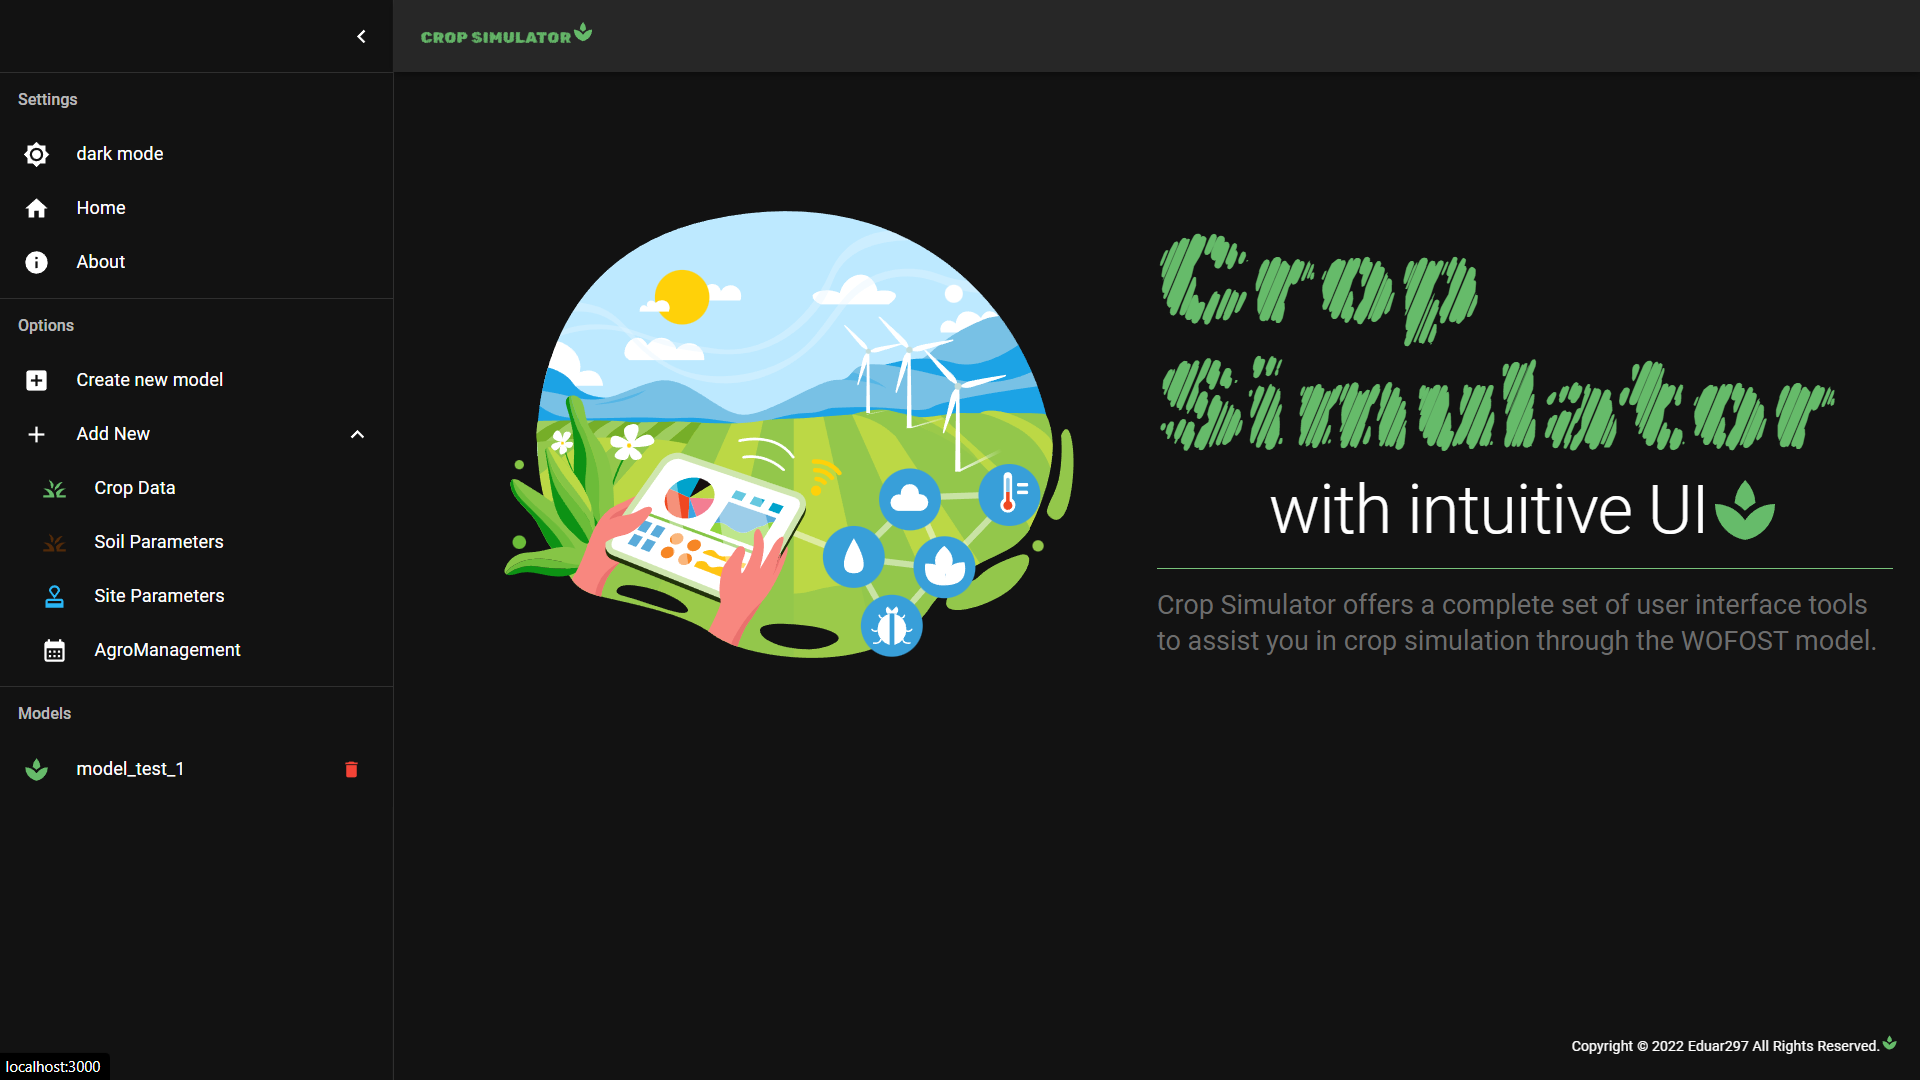
\includegraphics[width=0.6\linewidth]{Images/fron-home}
	\caption{Captura de pantalla de la página Home de la aplicación}
	\label{fig:fron-home}
\end{figure}

\begin{figure}[!h]
	\centering
	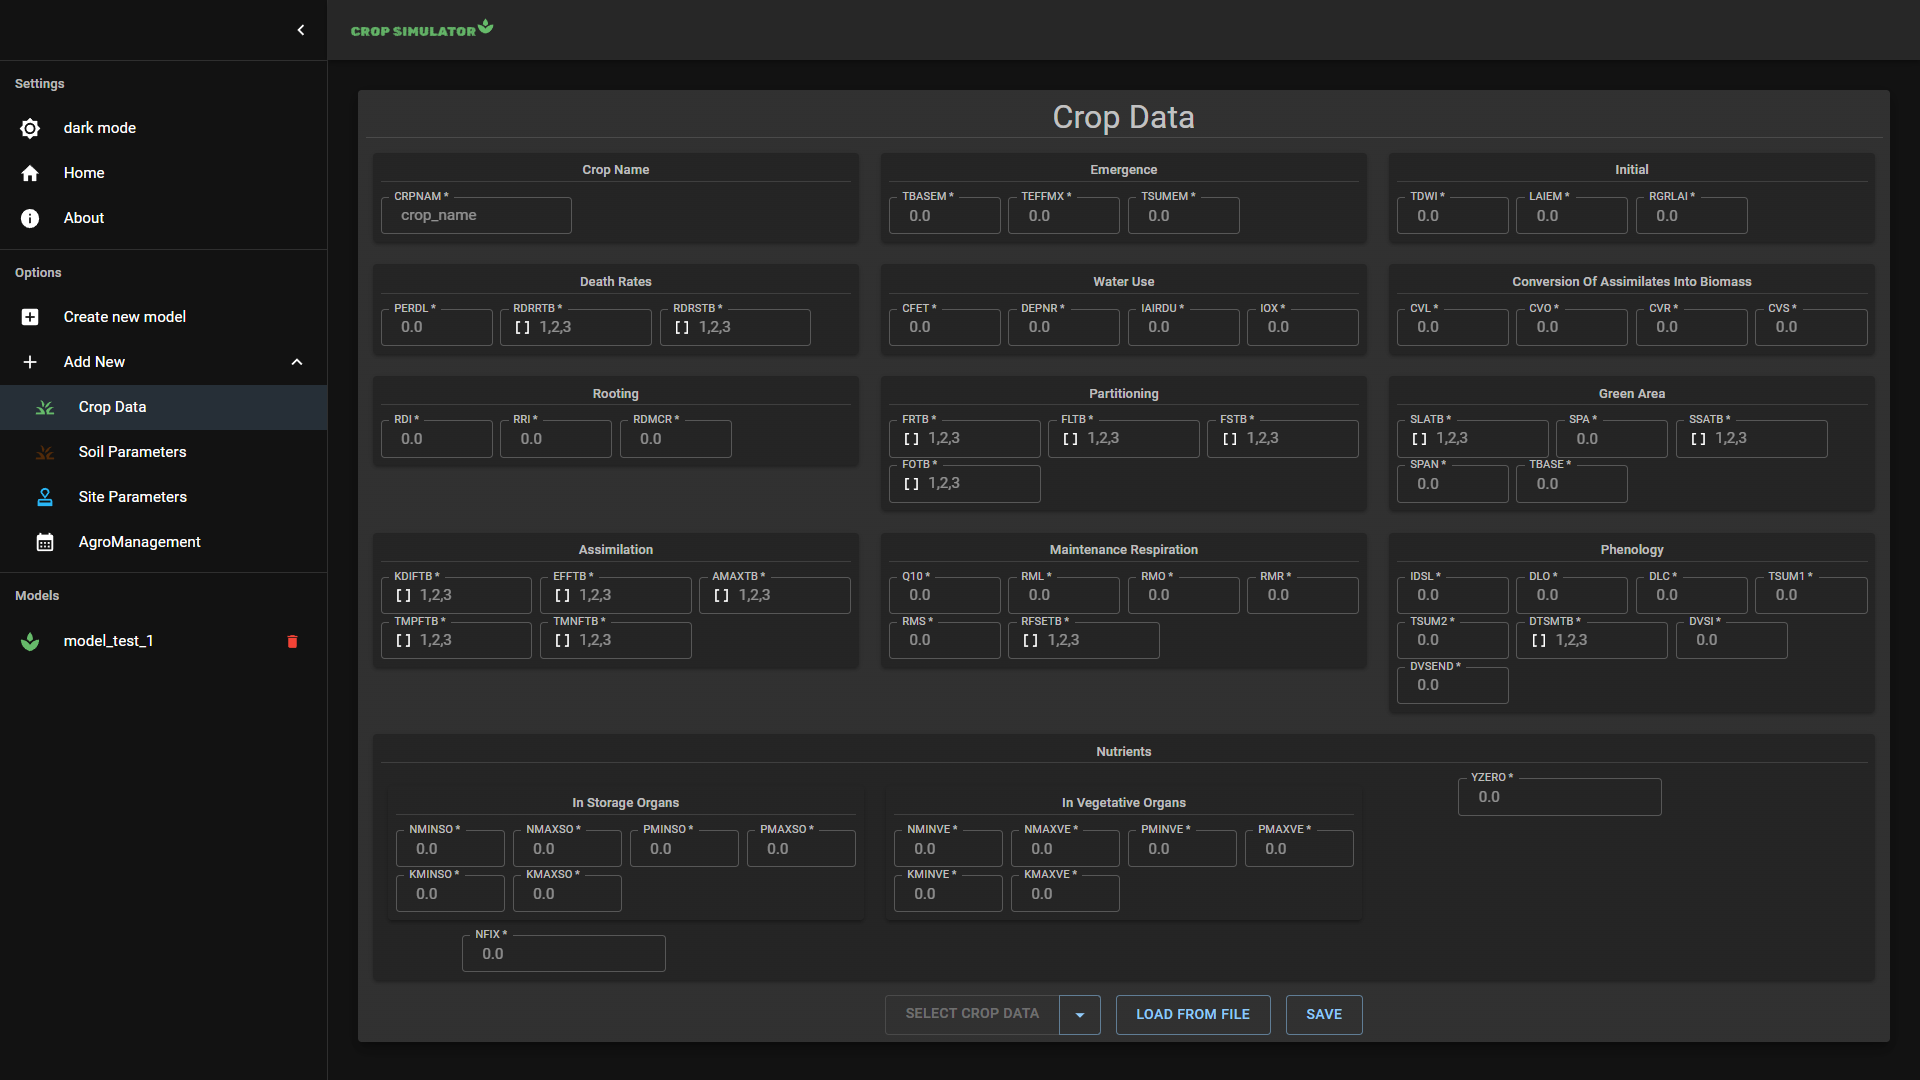
\includegraphics[width=0.6\linewidth]{Images/crop-page}
	\caption{Captura de pantalla de página Create Crop de la aplicación}
	\label{fig:crop-page}
\end{figure}

\begin{figure}[!h]
	\centering
	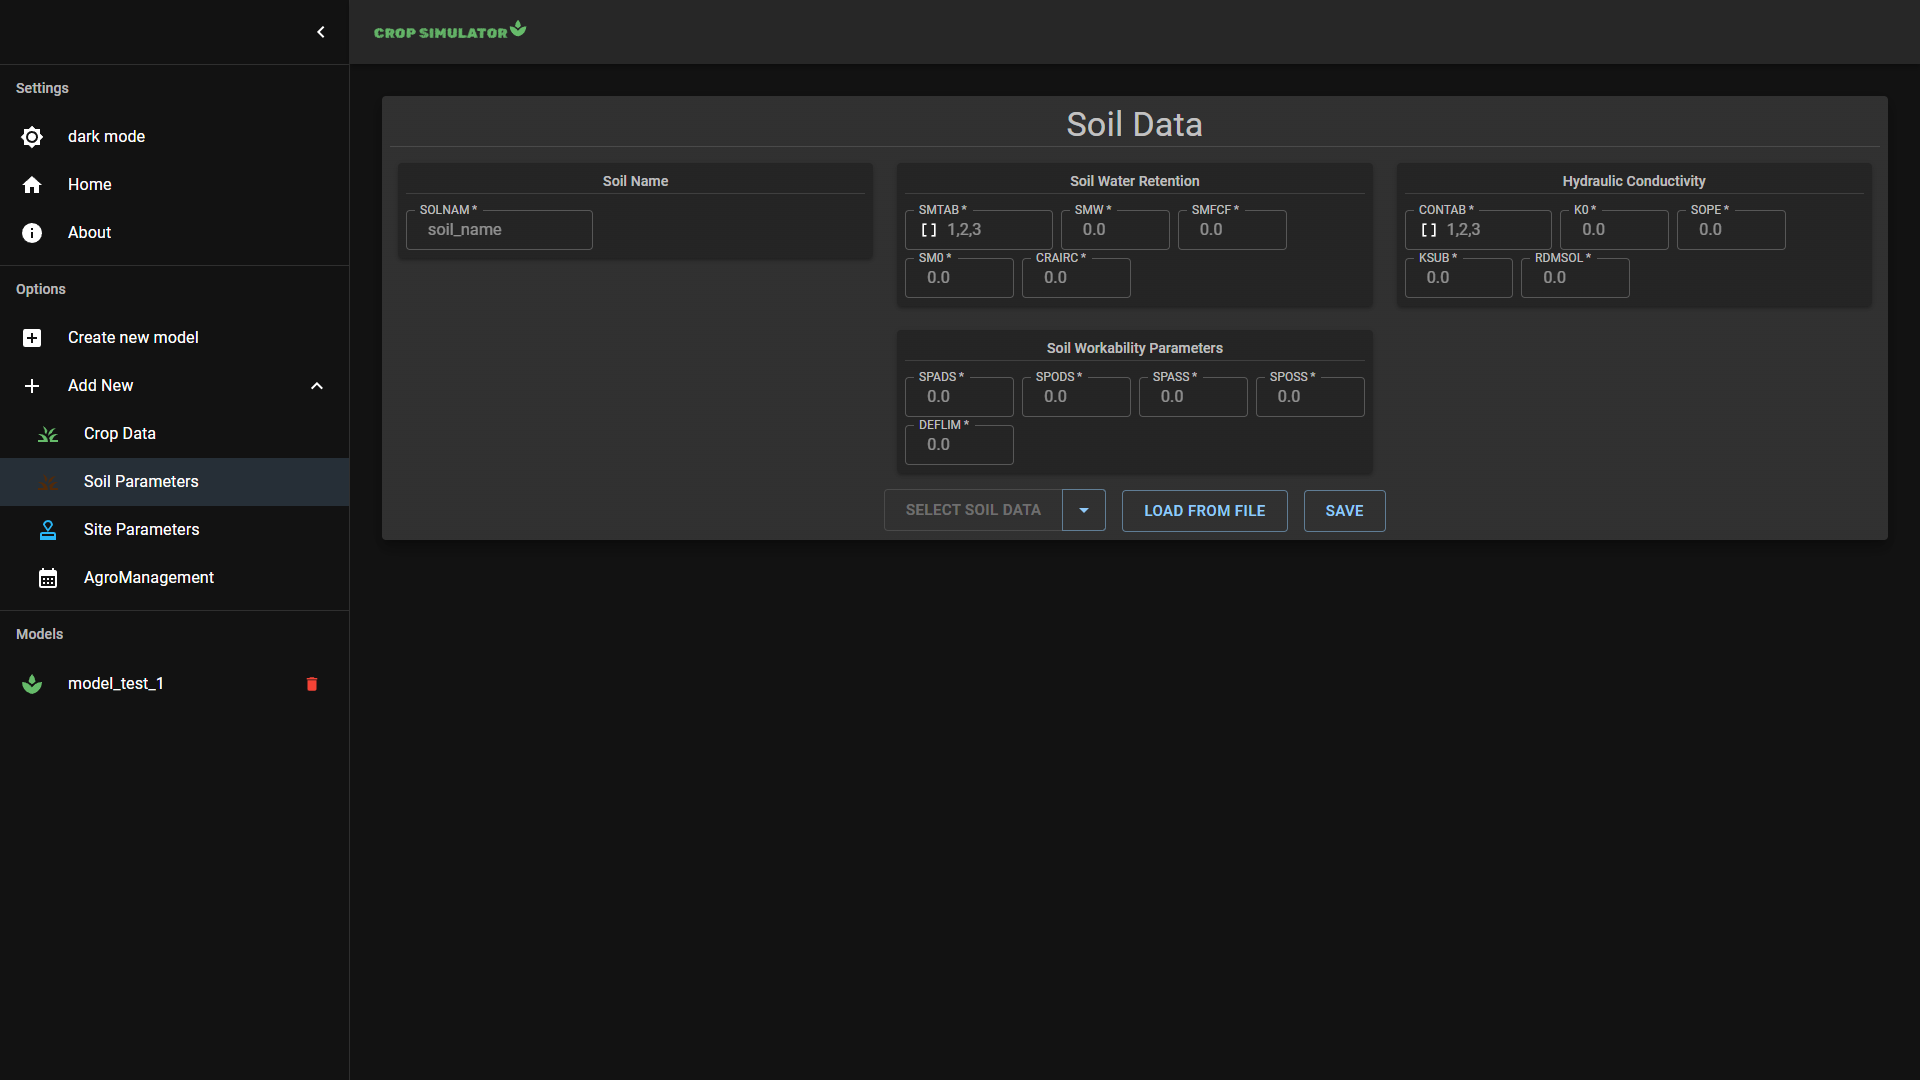
\includegraphics[width=0.6\linewidth]{Images/soil-page}
	\caption{Captura de pantalla de página Create Soil de la aplicación}
	\label{fig:soil-page}
\end{figure}

\begin{figure}[!h]
	\centering
	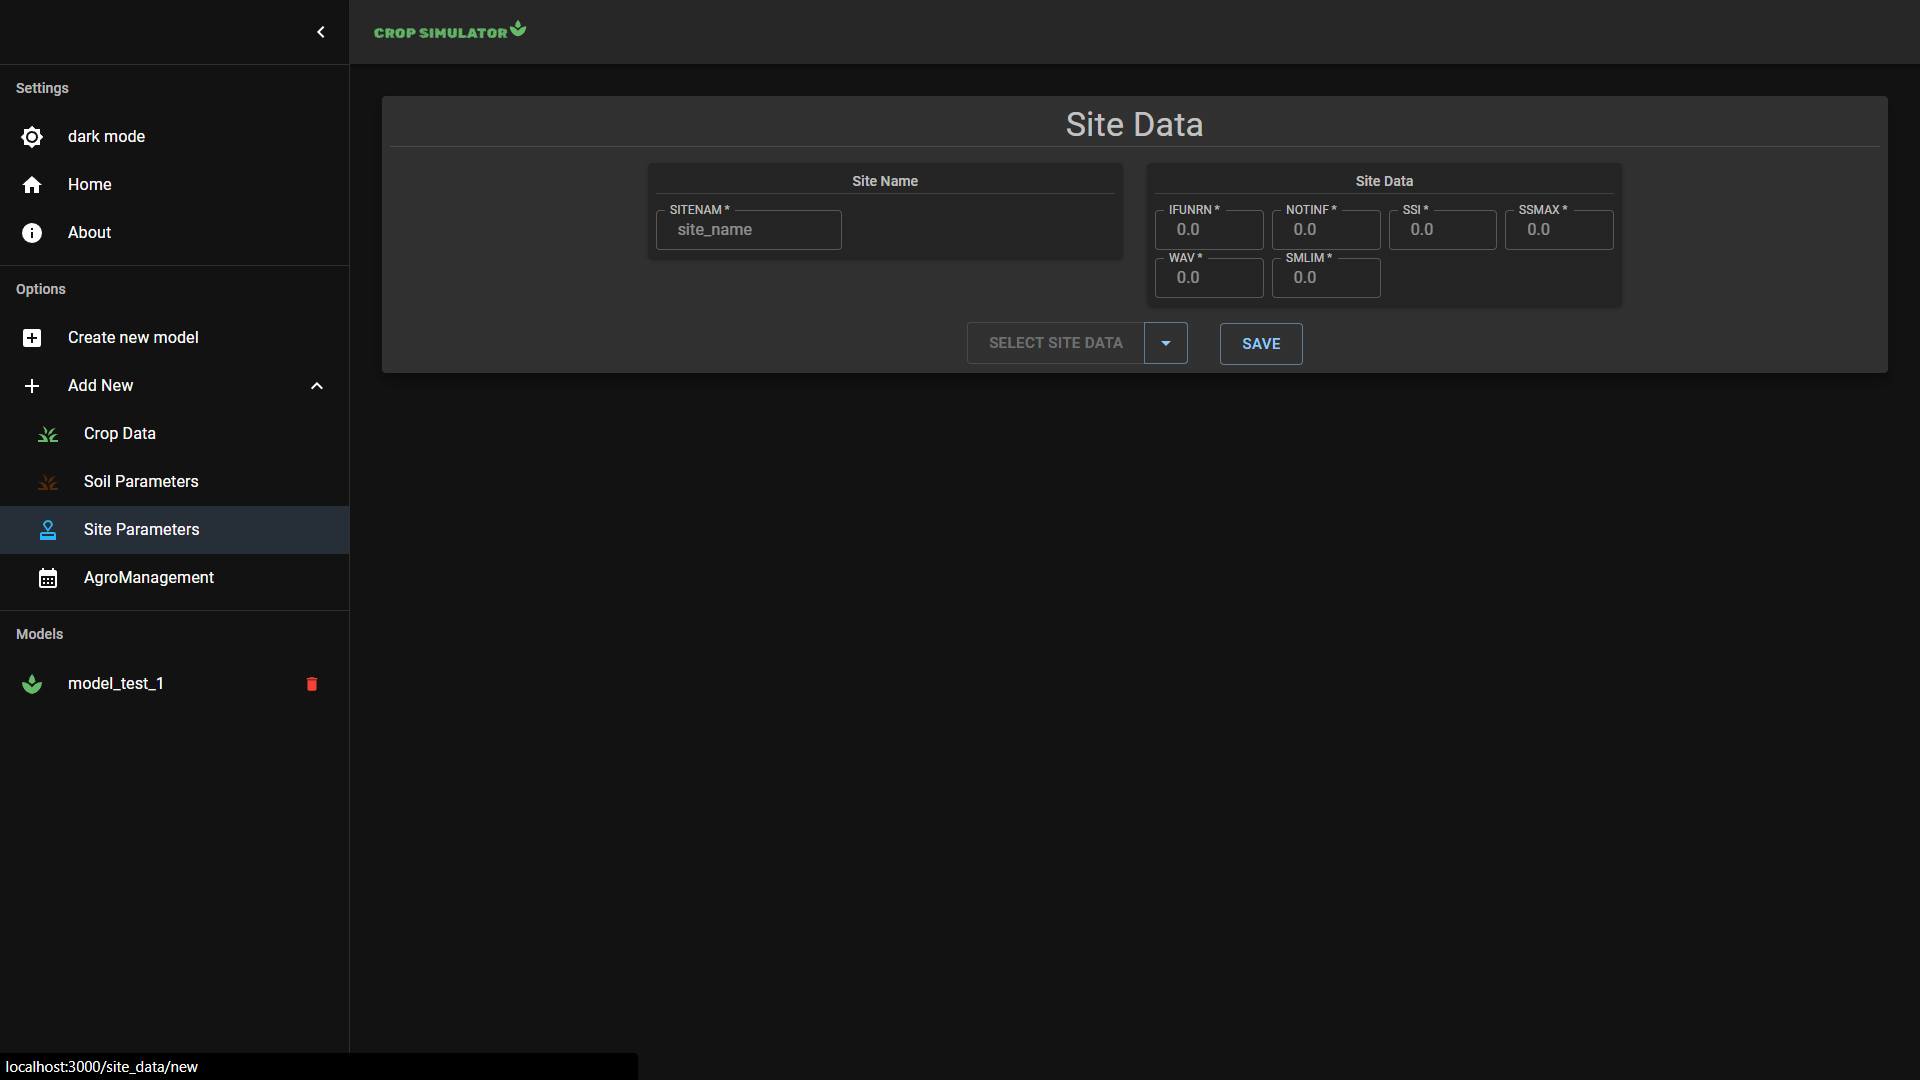
\includegraphics[width=0.6\linewidth]{Images/site-page}
	\caption{Captura de pantalla de página Create Site de la aplicación}
	\label{fig:site-page}
\end{figure}

\begin{figure}[!h]
	\centering
	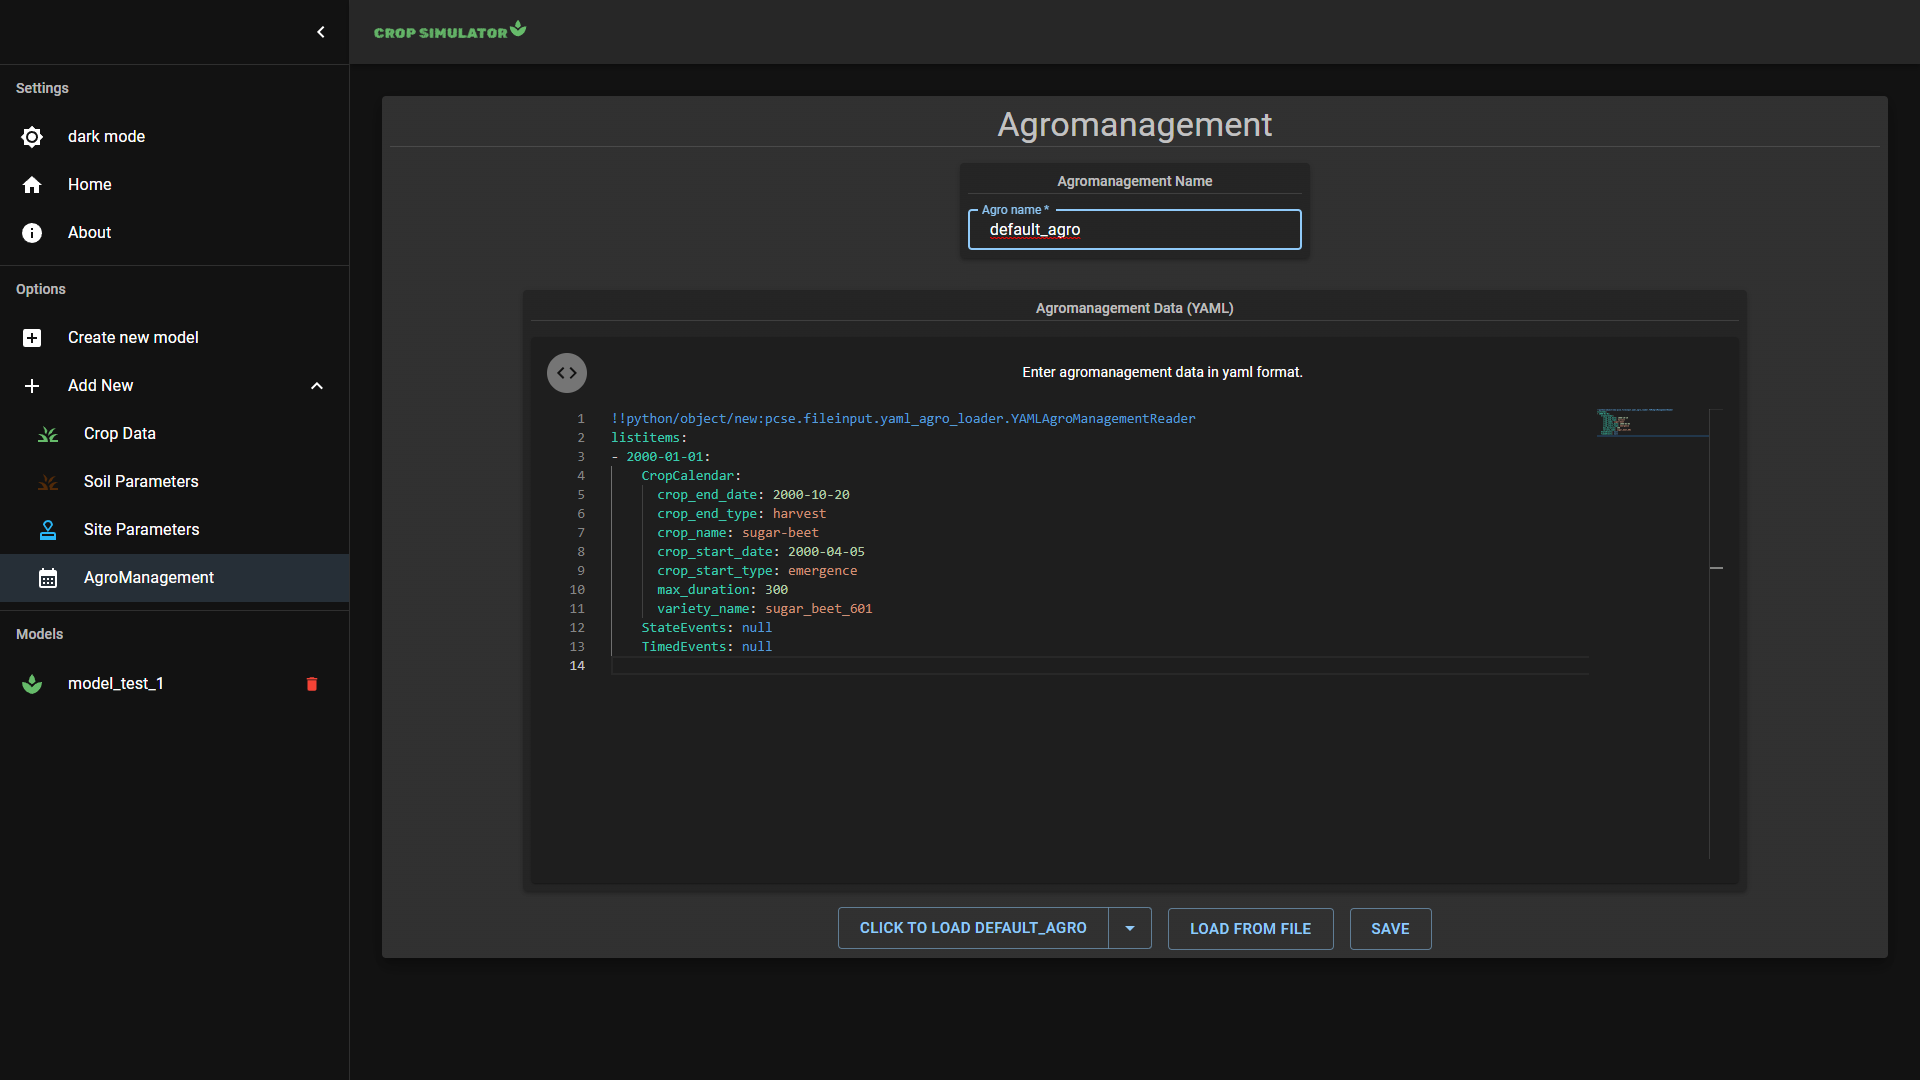
\includegraphics[width=0.6\linewidth]{Images/agro-page}
	\caption{Captura de pantalla de página Create Agromanagement de la aplicación}
	\label{fig:agro-page}
\end{figure}

La aplicación consta de una página Home (figura \ref{fig:fron-home}); un apartado para añadir datos de suelo, cultivo, sitio y calendario (figuras \ref{fig:crop-page}, \ref{fig:soil-page}, \ref{fig:site-page}, \ref{fig:agro-page} ).\\

En los apartados mencionados anteriormente, se pueden crear, cargar o modificar los datos iniciales de la simulación. En resumen, cada una de estas páginas consta de formularios. Una vez que el usuario llene todos los campos o cargue los datos, ya sea de un archivo o de la base de datos para modificar, estos tienen un método encargado de manejarlos y enviarlos al backend mediante \lstinline|axios| para ser procesados. 

Una vez creados todos los datos iniciales de la simulación lo siguiente será crear una instancia del modelo a simular, para esto se tiene la página Create new model, que es un formulario de tipo Stepper. De esta forma se va guiando e informando al usuario paso a paso de los datos que espera recibir para poder posteriormente comenzar la simulación.
\begin{figure}
	\centering
	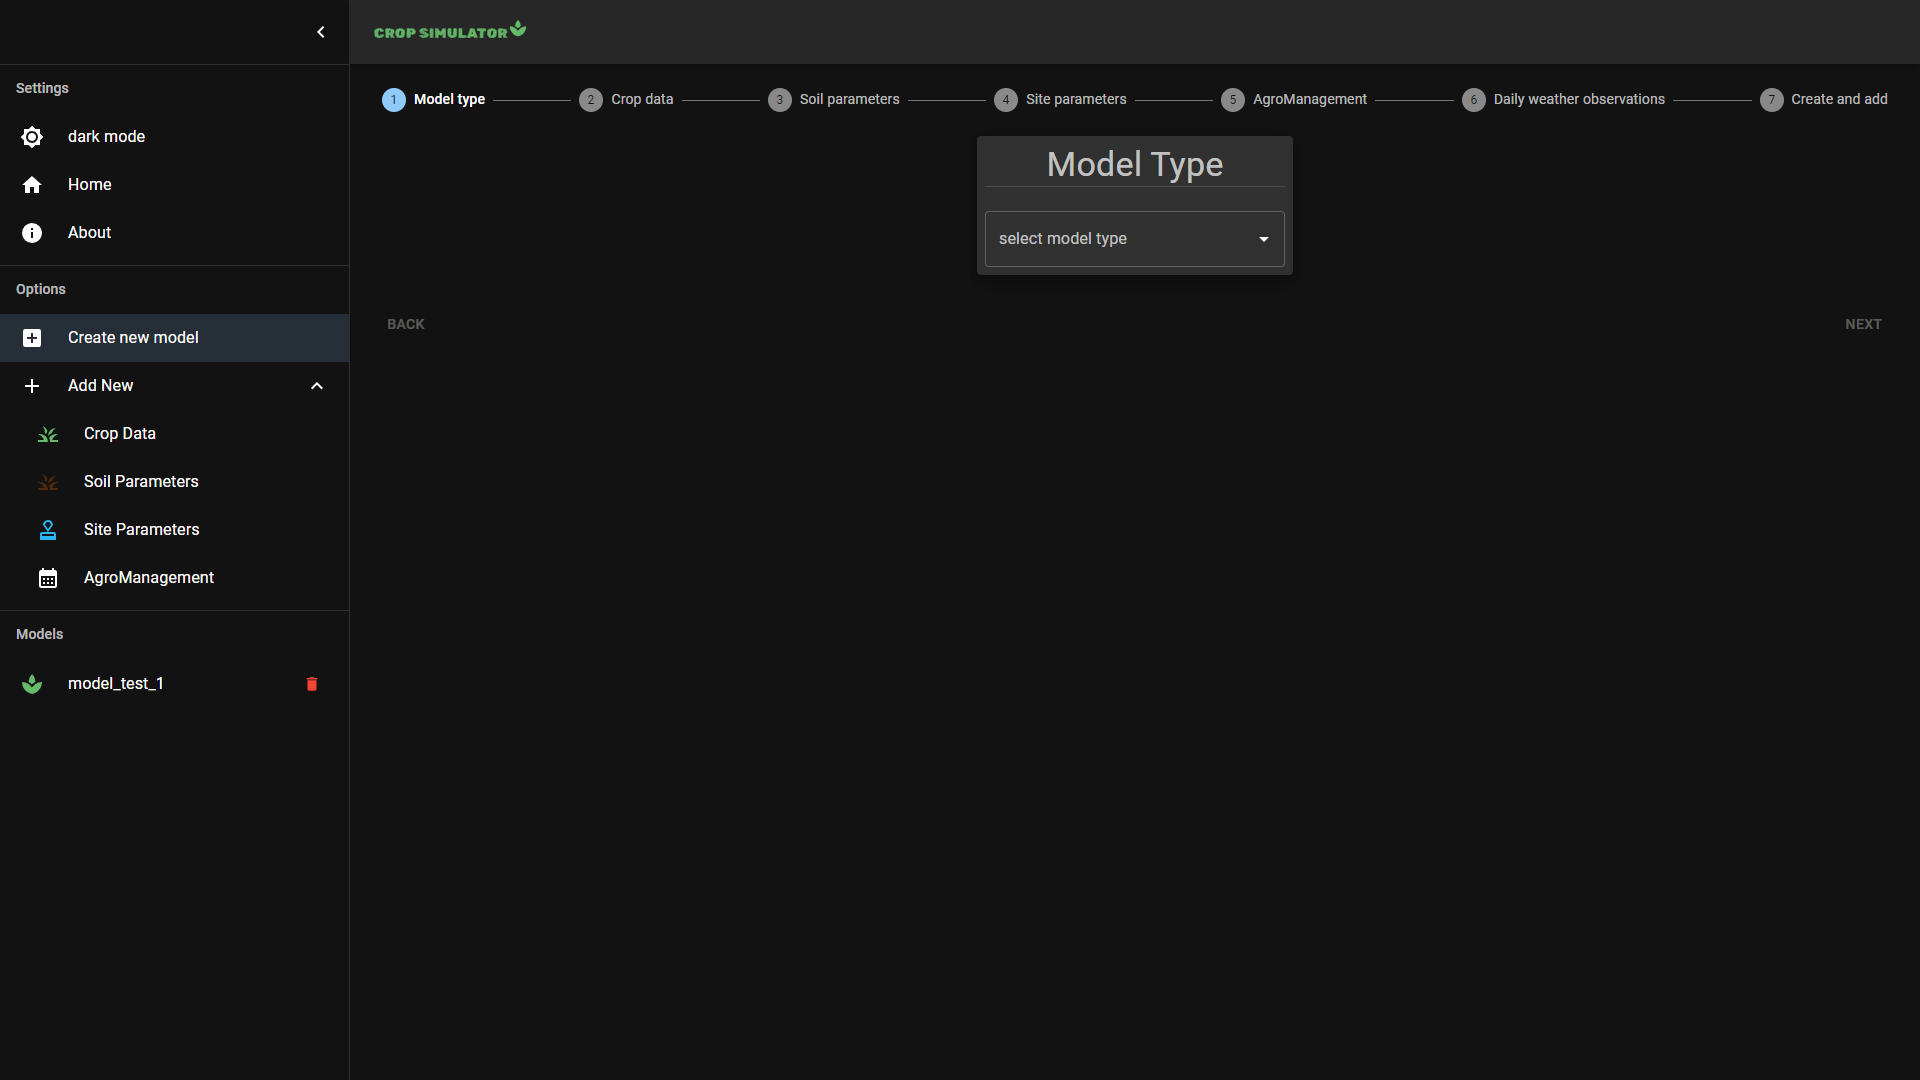
\includegraphics[width=0.5\linewidth]{Images/stepper-1}
	\caption{Model Type}
	\label{fig:stepper-1}
\end{figure}
El primer paso es elegir el tipo de modelo, para esto se pide a la api todos los posibles modelos. Luego se pide la data del cultivo, que puede haber sido creada con anterioridad y cargada de un archivo externo (en este caso se puede modificar o no) o crear una nueva. En los pasos siguientes se realiza la misma acción, pero exigiendo datos de suelo, sitio y calendario. Este último tiene una forma especial de crearse y es mediante la entrada en formato YAML, por ejemplo:

\begin{figure}[!h]
	\centering
	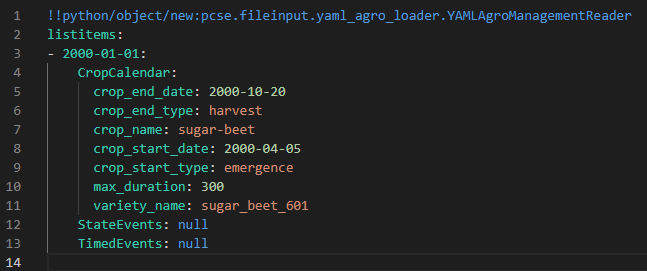
\includegraphics[width=0.4\linewidth]{Images/yaml-agro-eg}
	\caption{Ejemplo de agromanagement YAML}
	\label{fig:yaml-agro-eg}
\end{figure}

El paso final es suministrar al modelo parámetros climáticos, la manera de hacerlo es proveer la latitud y longitud de donde se quiere realizar el estudio, o simplemente, se puede usar la opción \lstinline|Geolocate me| que, si se le brindan los permisos al navegador, intentará calcular estos parámetros \lstinline|navigator.geolocation.getCurrentPosition|. En la siguiente figura se ve un ejemplo:

\begin{figure}[!h]
	\centering
	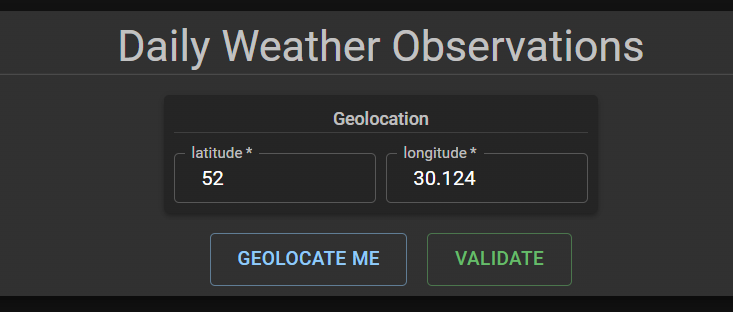
\includegraphics[width=0.4\linewidth]{Images/dwp}
	\caption{Ejemplo de geo-localización}
	\label{fig:dwp}
\end{figure}

Una vez tenemos todos los datos anteriores, se puede proceder al último paso, crear el modelo, para esto sólo se solicita el nombre del nuevo modelo y se muestra toda la información antes configurada, ejemplo:

\begin{figure}[!h]
	\centering
	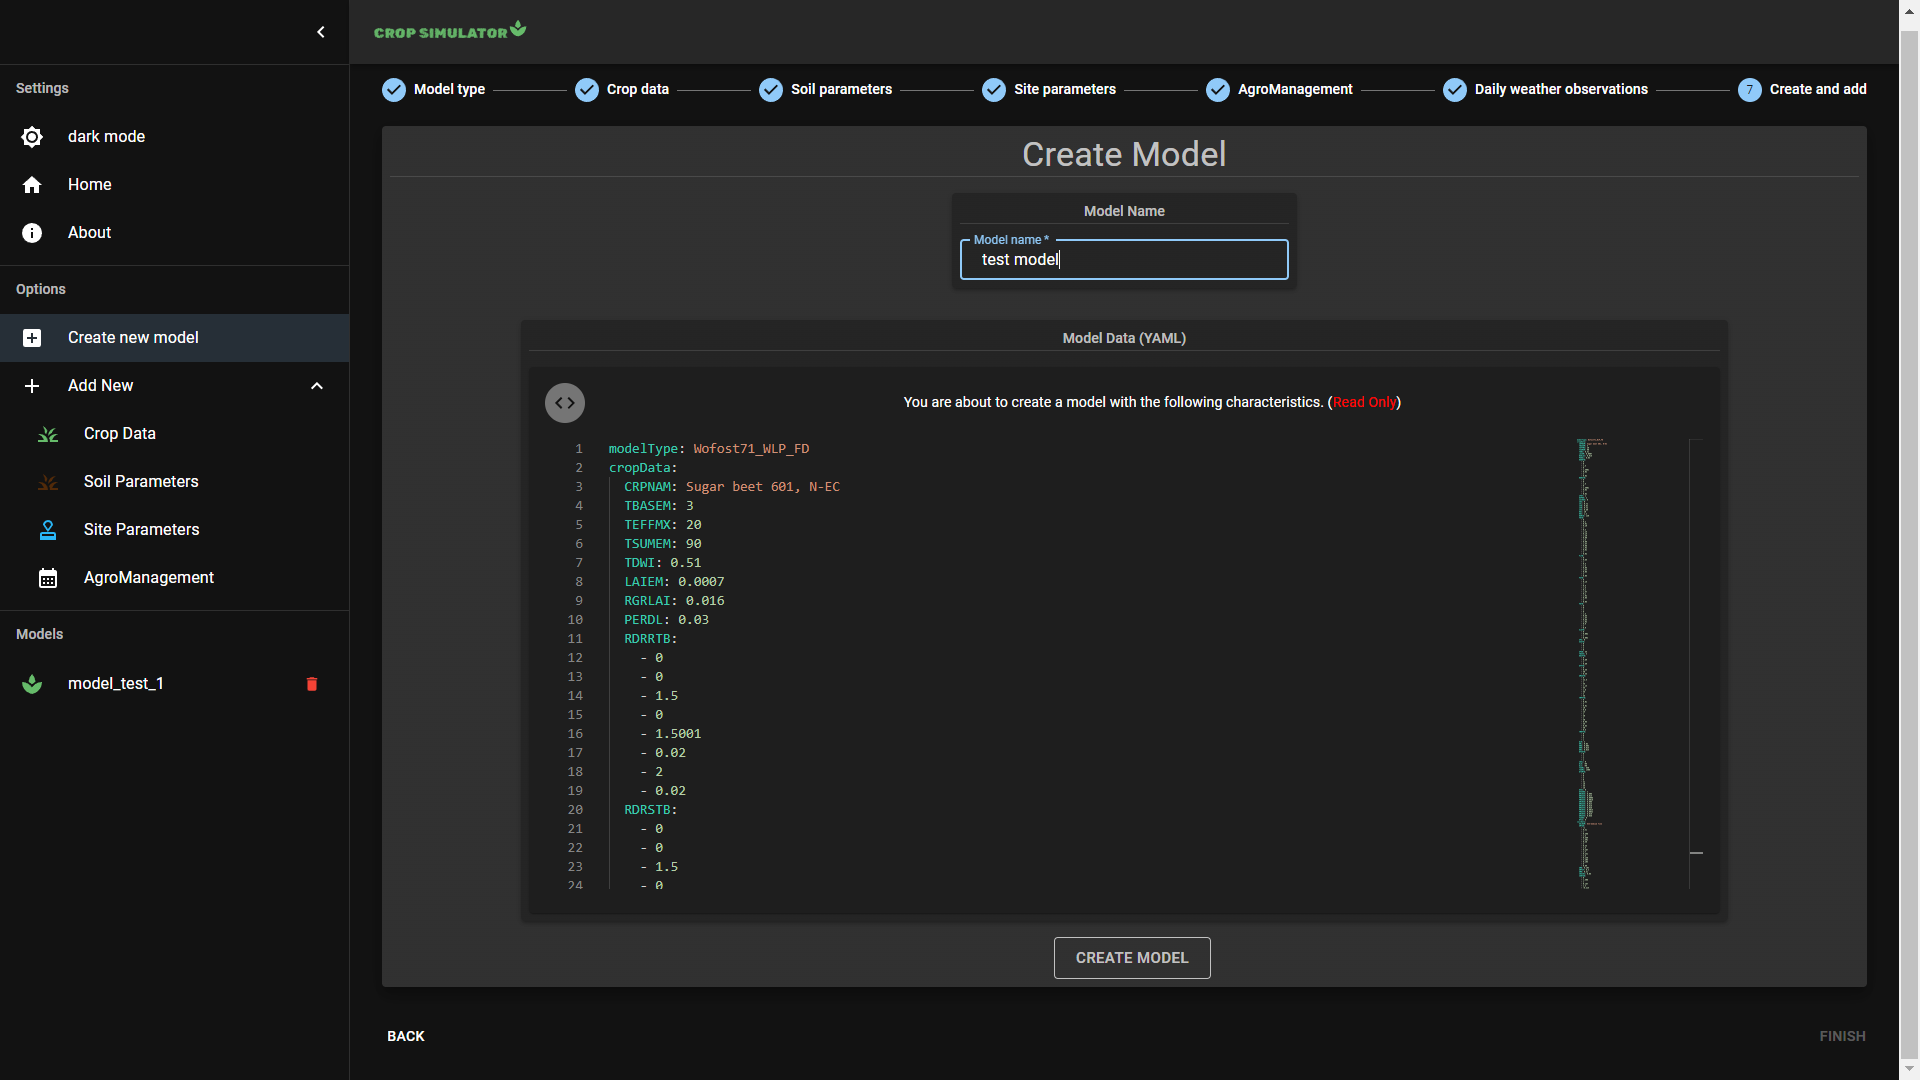
\includegraphics[width=0.5\linewidth]{Images/create-model}
	\caption{Ejemplo de crear modelo}
	\label{fig:create-model}
\end{figure}

Luego de aceptar, será creado un nuevo modelo con todo un conjunto de parámetros iniciales antes proveídos, listo para su simulación. No hay que preocuparse por los datos climáticos dado que al pedir valores de latitud y longitud, el servidor backend, usando la función \lstinline|NASAPowerWeatherDataProvider(latitude, longitude)| de \lstinline|pcse.db|, realiza una petición a la api de NASA Power para proveer estos datos climáticos.\\

Con el modelo ya creado con anterioridad, en el Sidebar en la última sección Models, aparece una lista con todos los modelos creados. Si todo salió bien, una vez creado el modelo, la aplicación redirigirá al usuario a una página con herramientas para poder llevar a cabo la simulación.

El primer apartado es para mostrar a detalle todos los parámetros iniciales de la simulación.
\begin{figure}[!h]
	\centering
	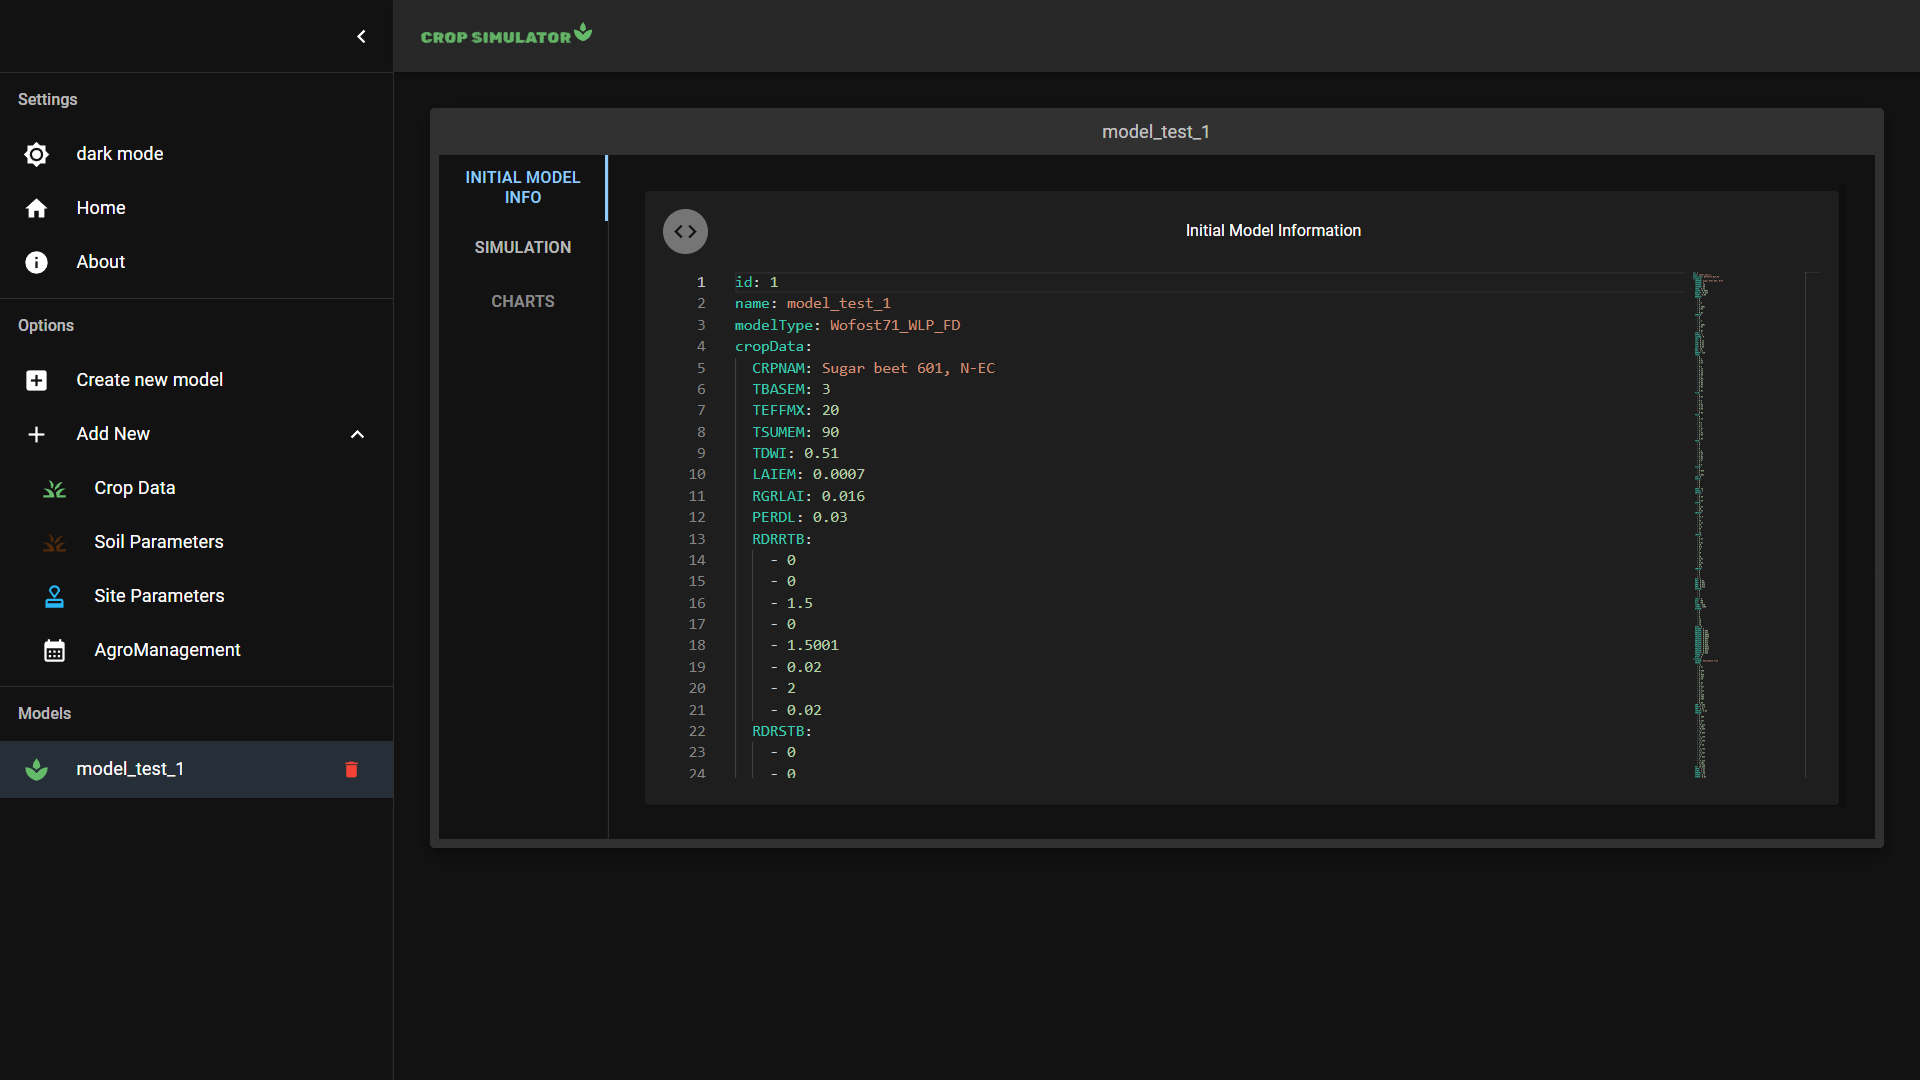
\includegraphics[width=0.5\linewidth]{Images/sim-1}
	\caption{Información del modelo. Parámetros iniciales}
	\label{fig:sim-1}
\end{figure}

El segundo apartado, Simulation, es la interfaz para interactuar con el modelo, o sea, correr, parar, setear variables de estado, iniciar el entorno de simulación, reiniciar. EL botón run $ i $ days tiene un select para seleccionar la cantidad de días que se desea simular, en cada iteración se hace una petición a la api, corriendo esta el modelo y retornando las variables de estado como son el LAI, SM, DVS, entre otras. Las variables se muestran en una tabla como se ve a continuación:

\begin{figure}[!h]
	\centering
	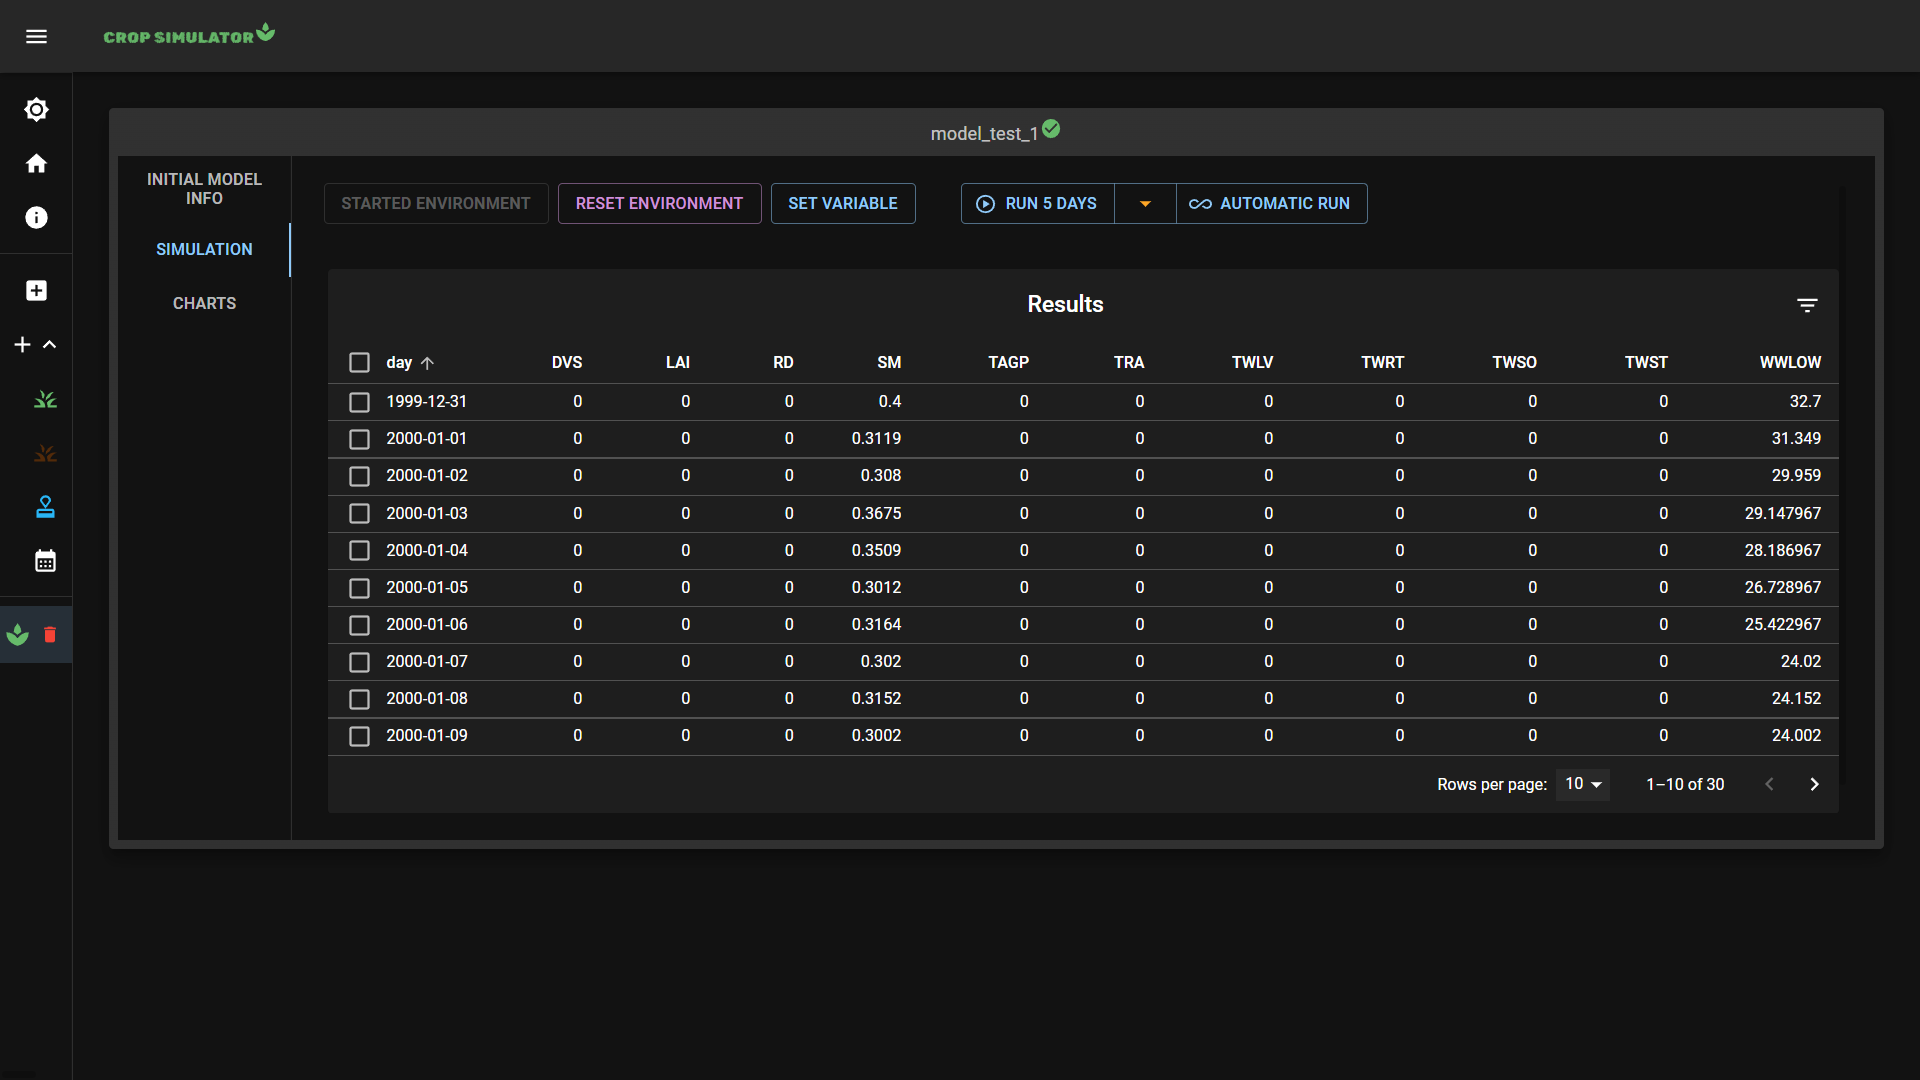
\includegraphics[width=0.6\linewidth]{Images/table}
	\caption{Ejemplo de dashboard de simulación}
	\label{fig:table}
\end{figure}

Dicha tabla permite ordenar todo el conjunto de variables por cualquier campo.

Finalmente, el apartado Charts muestra gráficas de todas las variables juntas o de cada una en específico, siendo el primero gráfico muy personalizable dado que se puede elegir cuáles variables ver y cuáles no.

Ejemplos (figura \ref{fig:tables}):\\

\begin{figure}[!h]
	\centering
	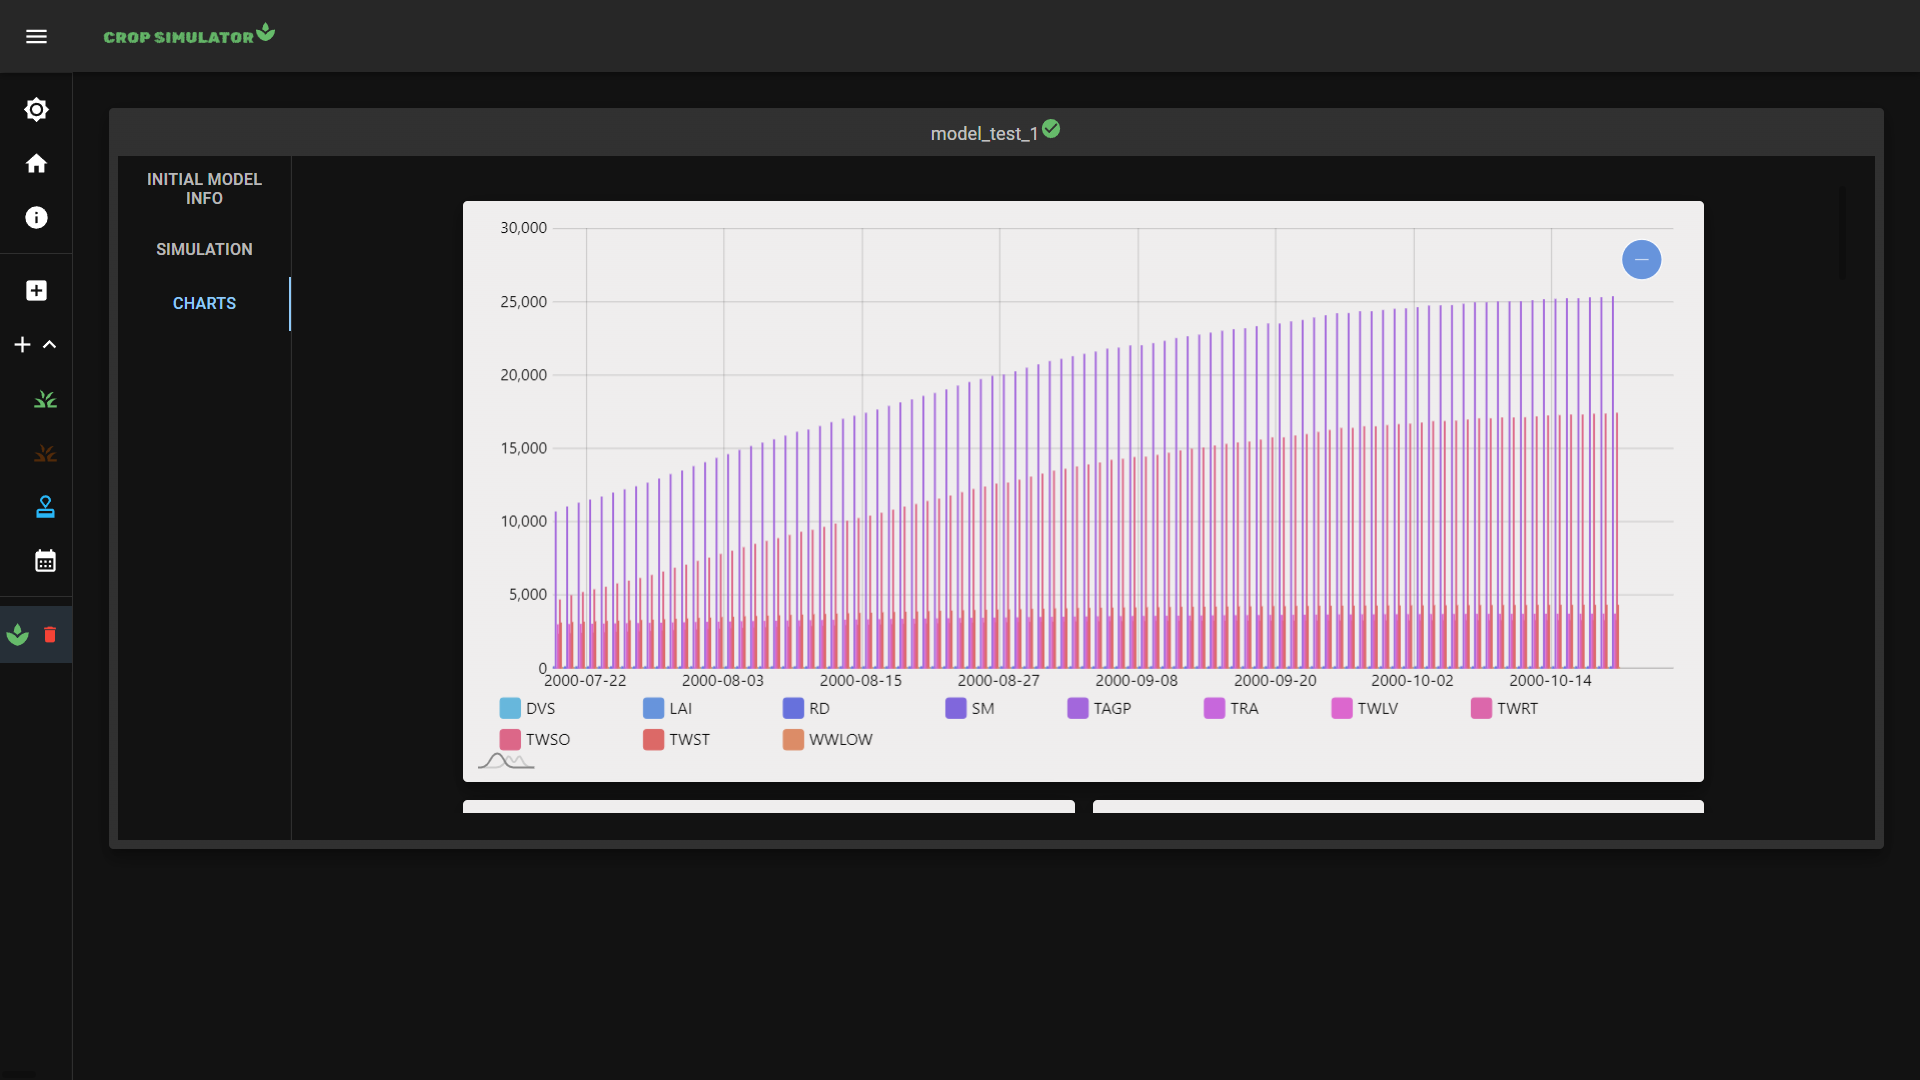
\includegraphics[width=0.4\linewidth]{Images/table1}
	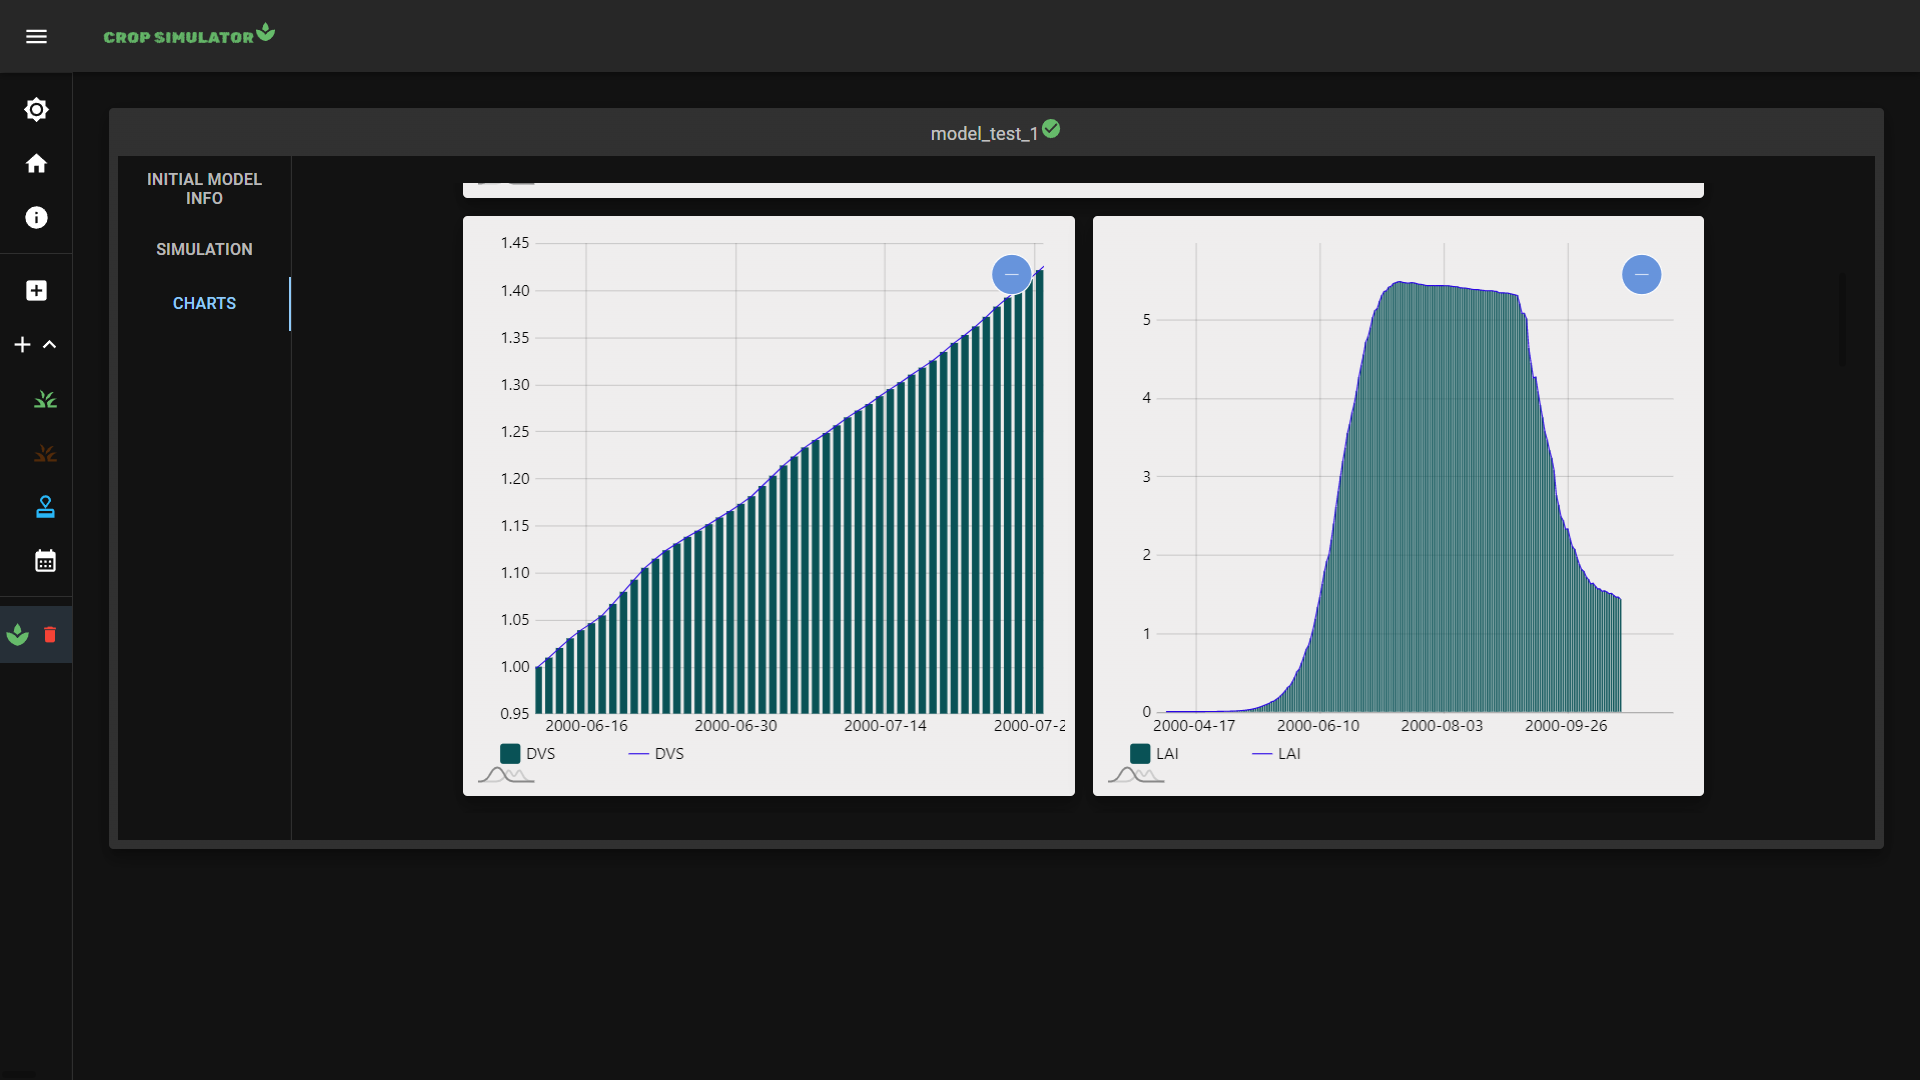
\includegraphics[width=0.4\linewidth]{Images/table2}
	\caption{Ejemplos de algunas gráficas de variables de estado}
	\label{fig:tables}
\end{figure}


A modo de resumen, la interfaz brinda la posibilidad de no tener que preocuparse por escribir código para poder simular el desarrollo de los cultivos, ni de realizar peticiones directamente a la api, pudiendo ser usada por personas no expertas en estos temas. Brinda un conjunto de herramientas para gestionar la simulación, analizar los valores diarios o finales, entre otras funcionalidades anteriormente descritas.

\section{Experimentación y exposición de resultados finales.} \label{chapter:implementation:results}
En este apartado se describe paso a paso un análisis de la simulación de un cultivo de remolacha azucarera calibrada en Alemania, norte y centro de Francia, Países Bajos, Bélgica, Luxemburgo, Reino Unido, Irlanda y Dinamarca con fecha de siembra entre el 1 y el 10 de abril y una fecha de cosecha entre el 17 y el 27 de octubre. 

Se muestran los parámetros iniciales a continuación.

\begin{python}
cropData:
	CRPNAM: Sugar beet 601, N-EC
	TBASEM: 3
	TEFFMX: 20
	TSUMEM: 90
	TDWI: 0.51
	LAIEM: 0.0007
	RGRLAI: 0.016
	PERDL: 0.03
	RDRRTB:[0,0,1.5,0,1.5001,0.02,2,0.02]
	RDRSTB:[0,0,1.5,0,1.5001,0.02,2,0.02]
	CFET: 1
	DEPNR: 2
	IAIRDU: 0
	IOX: 0
	CVL: 0.72
	CVO: 0.82
	CVR: 0.72
	CVS: 0.69
	RDI: 10
	RRI: 1.2
	RDMCR: 120
	FRTB:[0,0.2,0.91,0.29,1,0.3,1.15,0.15,
			1.29,0.09,1.3,0.09,1.57,0.08,1.92,0.01,2,0.02]
	FLTB:[0,0.85,1,0.5,1.3,0.05,1.57,0.05,2,0.05]
	FSTB:[0,0.15,1,0.5,1.3,0.1,1.57,0.1,1.92,0.05,2,0.05]
	FOTB:[0,0,1,0,1.3,0.85,1.57,0.85,1.92,0.9,2,0.9]
	SLATB:[0,0.002,2,0.002]
	SPA: 0
	SSATB: [0,0,2,0]
	SPAN: 35
	TBASE: 3
	KDIFTB:[0,0.69,2,0.69]
	EFFTB:[0,0.45,40,0.45]
	AMAXTB:[0,22.5,1,45,1.13,45,1.8,36,2,36]
	TMPFTB:[0,0.01,3,0.01,10,0.8,15,1,20,1,30,0.95,35,0.83,40,0.6]
	TMNFTB: [0,0,3,1]
	Q10: 2
	RML: 0.03
	RMO: 0.003
	RMR: 0.015
	RMS: 0.015
	RFSETB: [0,1,2,1]
	IDSL: 0
	DLO: -99
	DLC: -99
	TSUM1: 650
	TSUM2: 1400
	DTSMTB:[0,0,3,0,21,18,35,18]
	DVSI: 0
	DVSEND: 3
	NMINSO: 0.006
	NMAXSO: 0.013
	PMINSO: 0.0008
	PMAXSO: 0.0018
	KMINSO: 0.006
	KMAXSO: 0.013
	NMINVE: 0.018
	NMAXVE: 0.028
	PMINVE: 0.0015
	PMAXVE: 0.0032
	KMINVE: 0.018
	KMAXVE: 0.036
	YZERO: 0
	NFIX: 0
\end{python}

Los parámetros de suelo usados son de arena medianamente fina que se suelen usar para el balance de agua de suelos de drenaje libre. Se muestran a continuación los resultados.

\begin{python}
soilData:
	SOLNAM: EC3-medium fine
	SMTAB:[-1,0.41,1,0.398,1.3,0.389,1.491,0.38,2,0.34,2.4,
			0.287,2.7,0.241,3.4,0.148,4.204,0.104,6,0.09]
	SMW: 0.104
	SMFCF: 0.3
	SM0: 0.41
	CRAIRC: 0.06
	CONTAB:[0,1.408,1,0.167,1.3,-0.215,1.491,-0.638,1.7,-0.854,
			2,-1.155,2.4,-1.796,2.7,-2.26,3,-2.745,3.4,-3.357,
			3.7,-3.824,4,-4.276,4.204,-4.678]
	K0: 25.586
	SOPE: 1.47
	KSUB: 1.47
	RDMSOL: 80
	SPADS: 0.1
	SPODS: 0.03
	SPASS: 0.2
	SPOSS: 0.05
	DEFLIM: -0.3
\end{python}

Parámetros de sitio usados:

\begin{python}
siteData:
	SITENAM: default_site
	IFUNRN: 0
	NOTINF: 0
	SSI: 0
	SSMAX: 0
	WAV: 100
	SMLIM: 0.4
\end{python}

Parámetros de administración agrónoma:

\begin{python}
Version: 1.0
AgroManagement:
- 2000-01-01:
	CropCalendar:
		crop_name: 'sugar-beet'
		variety_name: 'sugar_beet_601'
		crop_start_date: 2000-04-05
		crop_start_type: emergence
		crop_end_date: 2000-10-20
		crop_end_type: harvest
		max_duration: 300
	TimedEvents: null
	StateEvents: null
\end{python}

Parámetros de geo-localización:

\begin{python}
geolocationData:
	latitude: 38.9847719
	longitude: -77.5619419
\end{python}

Una vez introducidos estos parámetros iniciales, se procedió a simular los primeros 5 días del cultivo, dando como resultado la tabla (\ref{fig:5d-table})

\begin{figure}[!h]
	\centering
	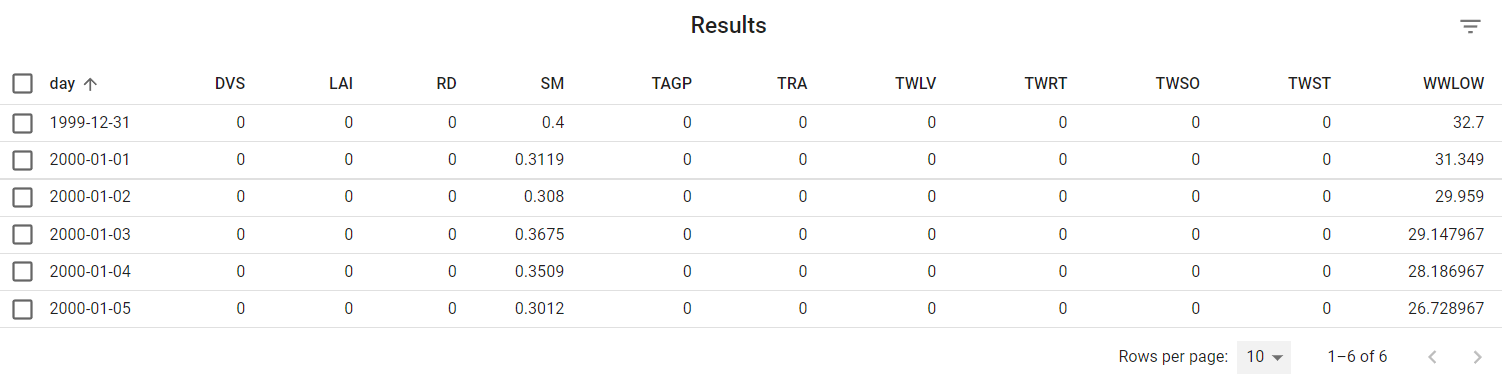
\includegraphics[width=1\linewidth]{Images/5d-table}
	\caption{Variables de estado de los primeros 5 días de simulación}
	\label{fig:5d-table}
\end{figure}

Como se puede apreciar en la tabla (\ref{fig:5d-table}) y las gráficas mostradas en la figura (\ref{fig:sm-chart-5d}), SM bajó de 0.4 a 0.3012 y WWLOW bajó de 32.7 a 26.728967 en el período de 5 días, las demás variables como el LAI aún se mantienen en 0.

\begin{figure}[!h]
	\centering
	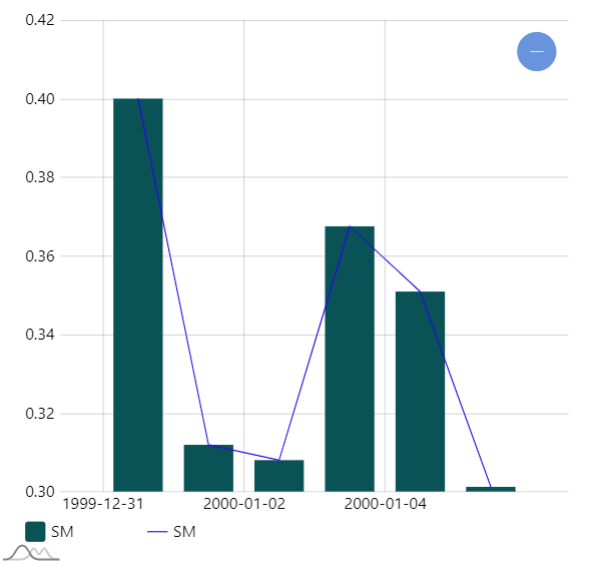
\includegraphics[width=0.4\linewidth]{Images/SM-chart-5d}
	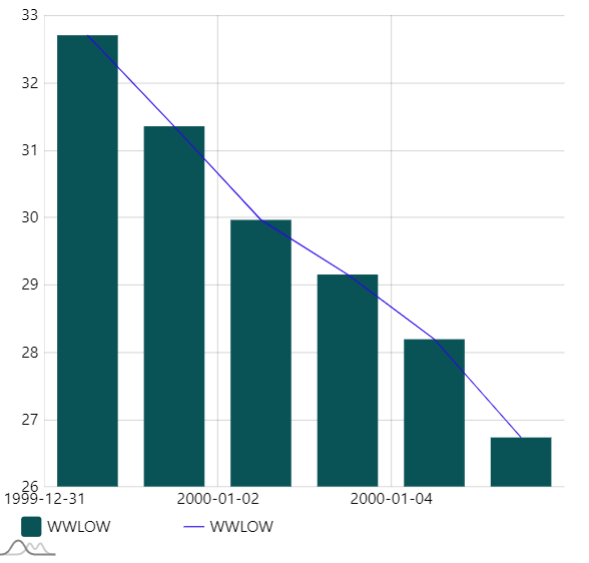
\includegraphics[width=0.4\linewidth]{Images/WWLOW-chart-5d1}
	\caption{}
	\label{fig:sm-chart-5d}
\end{figure}

Luego se procede a simular hasta el final de la campaña, la cual duró 294 días, y en este punto sí se aprecian grandes cambios en las variables de estado. Se muestran las variables LAI (índice de área foliar) y TAGP (total de biomasa) en las gráficas (\ref{fig:sm-chart-end})

\begin{figure}[!h]
	\centering
	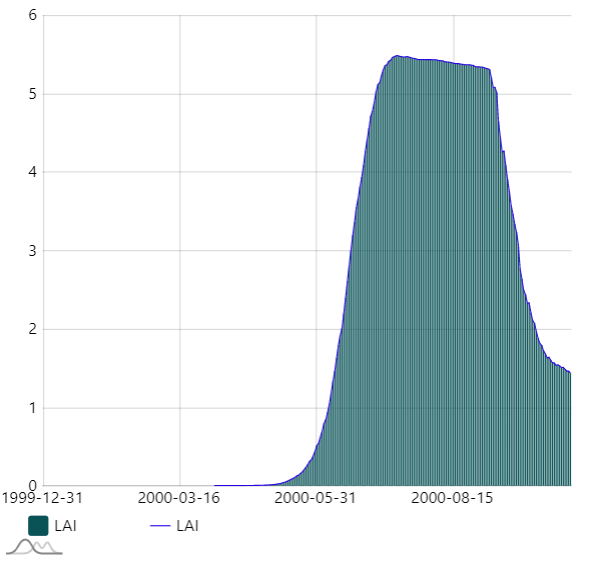
\includegraphics[width=0.4\linewidth]{Images/WWLOW-chart-5d6}
	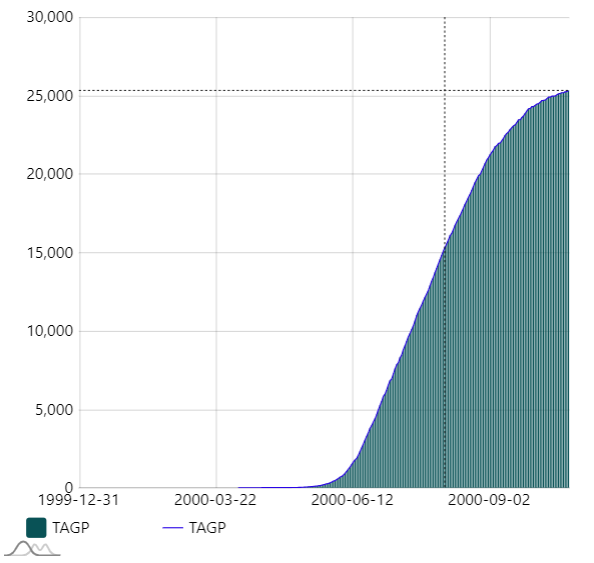
\includegraphics[width=0.4\linewidth]{Images/WWLOW-chart-5d7}
	\caption{LAI y TAGP}
	\label{fig:sm-chart-end}
\end{figure}

Como se puede apreciar, se creó una aplicación capaz de simular todo el proceso de simulación de cualquier cultivo siempre que sean proveídos todos los parámetros iniciales necesarios de suelo, sitio, cultivo, clima y manejo agroquímico.



















\backmatter

\begin{conclusions}
    La simulación y modelación en los últimos 25 años ha alcanzado gran auge e importancia, gracias a su efectividad y la gran cantidad de recursos que pueden ser ahorrados con esta. La simulación de cultivos específicamente permite estimar de manera bastante fiable el rendimiento de un cultivo.
    La presente investigación tomó como base el modelo WOFOST, encontrado en Python Crop Simulation Environment (PCSE). Este modelo permite estimar los valores de las variables biológicas como el rendimiento de los órganos de almacenamiento y la biomasa total.
    Se desarrolló una interfaz visual intuitiva que permite el trabajo con datos reales para su simulación y posterior análisis mediante el uso de tablas y gráficas. La aplicación permite al usuario simular una determinada cantidad de días, parar la simulación para cambiar algún estado de acuerdo a los datos reales y continuar con la simulación. Esto permite mejorar el modelo y obtener resultados más fiables gracias a la retroalimentación.
    Tanto el objetivo general de la investigación, así como los objetivos específicos propuestos en la misma fueron cumplidos satisfactoriamente, aunque se seguirá trabajando en futuras investigaciones.
\end{conclusions}

\begin{recomendations}
	En esta	investigación se realizó una simulación con datos de cultivos de remolacha y suelos de arena medianamente fina suministrados por la base de datos de WOFOST, dado que no fue posible la obtención de datos de cultivos específicos de Cuba. Por esta razón, se recomienda para futuras investigaciones utilizar datos de cultivos cubanos para calibrar el modelo y contrastar los datos obtenidos de la simulación con los datos reales para ver con qué nivel de precisión se logra estimar el rendimiento de los cultivos. Además, se recomienda seguir mejorando la aplicación, para añadir nuevas funcionalidades que faciliten aún más el trabajo con esta. Otra recomendación sería encontrar una forma de generar varias trayectorias del cultivo, así como la elección de estas mediante el uso de filtros de partículas.
\end{recomendations}

\include{BackMatter/Bibliography}

\end{document}